\documentclass[prodmode,acmtecs]{acmsmall} % Aptara syntax
%\documentclass[11pt]{article}

%\renewcommand{\baselinestretch}{1.5} 
\usepackage{latexsym}
\usepackage{graphicx}
\usepackage{color}
\usepackage{multirow}

\usepackage{graphicx}
\usepackage{color}
\usepackage{multirow}
\usepackage{amsmath}
\usepackage{amssymb}
\usepackage[font=small,labelfont=bf]{caption}


\usepackage[ruled,vlined,linesnumbered]{algorithm2e}
\renewcommand{\algorithmcfname}{ALGORITHM}
\SetAlFnt{\small}
\SetAlCapFnt{\small}
\SetAlCapNameFnt{\small}
\SetAlCapHSkip{0pt}
\IncMargin{-\parindent}



\usepackage{wrapfig}
\usepackage{algorithmic}
\usepackage{algorithm2e}
\usepackage{tikz}
\usepackage{hyperref}
\usepackage{subcaption}
%\usepackage{fullpage}
\usepackage{times}

%\newtheorem{definition}{Definition}

\newcommand{\note}[2]{\textbf{\textsc{#1} says: \textit{#2}}}
%\newcommand{\comment}[1]{}

\newcommand{\islead}[1]{{\em IsLead(#1)}}
\newcommand{\acquire}[1]{{\em Acquire(#1)}}
\newcommand{\target}{{\textit target}}
\newcommand{\best}{{\textit best}}
\newcommand{\pf}{{\textit pf}}



%\author{Liron Samama-Kachko, Roni Stern, Rami Puzis,  Ariel Felner} 
%\author{Liron Samama-Kachko, Rami Puzis, Roni Stern, and Ariel Felner} 

\title{TONIC: Target Oriented Network Intelligence Collection \\
{\large Efficient Exploration of Social Networks}}

\author{Liron Samama-Kachko, Barak Hagbi, Roni Stern, Rami Puzis,  Ariel Felner
\affil{Ben-Gurion University of the Negev}
}


\begin{document}


\markboth{Samama-Kachko et al.}{TONIC: Target Oriented Network Intelligence Collection}


%%%%%%%%%%%%%%%%%%%%%%%%%%%%%%%%%%%%%%%%%%%%%%%%%%%%%%%%%%%%%%%%%%%%%%%%%%%%%%%%%%%%%%%%%%%%%%%%%%%%%%%
\begin{abstract}
%\note{Rami}{abstract shortened to 100 words.}
The Target Oriented Network Intelligence Collection (TONIC) is optimized crawling process for finding leads, social network profiles that contain information about a given target.  Two best-first search frameworks are proposed for solving TONIC. When the reward of finding a lead is moderate and the cost of ``useless'' crawl is high we propose the Restricted TONIC Framework that limits the search to immediate neighbors of previously found leads. The Extended TONIC Framework extends the scope of the search to a wider neighborhood. Experimental analysis on the popular social networks shows that acquisition of non-leads significantly speeds up the search process. 


%\note{Roni}{I rewrote some parts of the abstract, and taken a lot from our recent SoCS paper.}
%The Target Oriented Network Intelligence Collection (TONIC) problem is the problem of finding profiles in a social network that contain information about a given target via automated crawling. Such profiles are called {\em leads}. Two best-first search frameworks are proposed for solving TONIC and several heuristics are proposed for each framework. 
% [R 3.3]
%The first proposed framework, called the Restricted TONIC Framework (RTF), limits the search for new leads only to immediate neighbors of the leads previously found. This is motivated by homophily principle -- people tend to be friends of other people with similar attributes. This principle is known to manifest in online social networks, and it translates  in our case to an assumption that leads tend to cluster together. The second proposed framework, called the Extended TONIC Framework (ETF), relaxes this limitation and extends the scope of the search to a wider neighborhood, including the possibility of crawling to profiles that are not leads.
%We analyze experimentally the pros and cons of the two frameworks on the popular Google+ social network. The results show that ETF can reach substantially more leads and in some cases even faster, but RTF might be preferred in cases where the reward of finding a lead is moderate and insufficient constraints may cause the search process to diverge.
%\note{Roni: this is wierd. If there is no constraint on the total cost of queries, then why not do ETF?}
%Our results also provide insight into different aspects of the TONIC problem, including the maximal number of leads that can be found and how topological characteristics of the social network affect the leads-finding process.

%Our results also provide insight into the maximal number of leads that can be found in each framework, topological characteristics that may effect the leads finding process and analysis of the TONIC problem from different aspects of the problem
%Our results also provide insight into the maximal distance that exists between two leads of the same target. \note{Roni}{Does the last sentence make sense? I mean to hint here towards the ``tiers'' table}

\end{abstract}
%%%%%%%%%%%%%%%%%%%%%%%%%%%%%%%%%%%%%%%%%%%%%%%%%%%%%%%%%%%%%%%%%%%%%%%%%%%%%%%%%%%%%%%%%%%%%%%%%%%%%%%

\maketitle

\section{Introduction}

% 1. OSNs are popular, and people use them to gather intelligence on other people
Web-based {\em online social networks} (OSNs) such as Facebook, Twitter, and Google+ are a part of everyday life for many people around the world. These OSNs are a source of personal information about their users and even contain sensitive commercial or security related information. Commercial companies, government agencies, and even individual people often utilize this abundance of data to extract information about a given person of interest. For example, it is common practice for most commercial companies to inspect the Facebook and LinkedIn profiles of candidate employees in order to extract information about past projects, colleagues, and managers. Government agencies may also explore OSNs looking for information on terrorists and organized crime. 

% 2. Information gathering can be automated, but people block this via privacy.
The process of collecting the information available in an OSN 
about a given person or group of interest can be automated using information extraction (IE) techniques \cite{chang2006survey}. We refer to such a person or group of interest as the $\target$. 
Awareness to privacy issues and to data leakage cause many users to tighten their OSN privacy settings limiting access to their profiles. Consequently, the target's profile is inaccessible to third parties and information about the target cannot be collected from its profile. Furthermore, there might be scenarios where the target does not even have an OSN profile, but information about the target is still available in the OSN.

% 3. If the target is blocked, we get information about it from other profiles. Introducing the notion of a lead. 
In such cases, an alternative way to collect information about the target is through information available in other OSN profiles. 
For example, information about the target can be collected also from profiles that contain photos of the target, public posts made by the target or posts made by other profiles about the target.
If the target has a profile in the OSN, then a likely source of information about the target is in the profiles of its acquaintances, where acquaintances can be defined using the OSN {\em friendship relationship}.   
It is prohibitively challenging to conceal information about the target that other profiles expose.
A profile that exposes information about the target is called a {\em lead}.



%Information about the target can be collected also from profiles that contain photos of the target, public posts made by the target or posts about the target.

% 4. The TONIC problem. 
In this paper we address the problem of finding as many leads as possible while minimizing the number of inspected profiles. We call this problem the {\em Target Oriented Network Intelligence Collection (TONIC)}. 
In our model, extraction and analysis of relevant information from the OSN is encapsulated in two operators: {\em IsLead} which is a light query that determines whether a profile is a {\em lead} or not, and {\em profile acquisition} which is a heavy operation that fully extracts and observes the information of a given profile.
%We make the assumption that extraction and analysis of relevant information from the OSN is encapsulated in two operators: {\em Islead} which is a light query that determines whether a profile is a {\em lead} or not, and {\em profile acquisition} which is a heavy operation that fully extracts and observes the information of a given profile.
We assume that these operators can be carried out by utilizing web scrapping or the OSN application programming interfaces (API) followed by standard IE techniques \cite{chang2006survey,tang2010aCombinationApproach,pawlas2012universal}.


% This is a search problem, we do BFS and have nice heuristics.
We solve TONIC with Artificial Intelligence techniques, formalizing it as a heuristic search problem.  Profiles and friendship relations form the vertices and edges of a  graph, respectively, and we use a best-first search approach to search this graph~\cite{vempaty1991depthFirst,russell2010artificialIntelligence}. We visit profiles in a best-first order according to heuristic functions that we develop in this paper and apply the {\em IsLead} and {\em profile acquisition} operators on the {\em best} profile in an intelligent manner. 


Two frameworks are proposed for solving TONIC, the Restricted TONIC Framework (RTF) and the Extended TONIC Framework (ETF). RTF restricts the search to known leads and their neighbors. Therefore, in RTF profiles that are found to be non-leads are omitted from deeper exploration. The rationale behind restricting acquisition of non-leads is that the cost of {\em profile acquisition} can be quite high and it may not result in the discovery new leads. 
By contrast, ETF does not restrict acquisition of non-leads and allows the search to continue through the extended social cycles of a target. As a generic middle ground between RTF and ETF, we proposed ETF($n$), in which non-leads are only explored if they are at most $n$ steps from a known lead. Thus RTF=ETF(0) and ETF= ETF($\infty$). 

Several intelligent heuristics are proposed for both RTF and ETF. These heuristics analyze the currently known subgraph of the OSN to guide the search. Importantly, all our investigated heuristics are based solely on the topology of the OSN being crawled, and are thus orthogonal to the details of the {\em IsLead} and {\em profile acquisition} operators. 


The proposed heuristics and frameworks are experimentally evaluated on three OSNs: Google+, Pokec~\cite{takac2012data}, and LiveJournal~\cite{backstrom2006groupFormation,leskovec2009community} (an online community that allows member to maintain journals, blogs, and define friendship between profiles). Results show that each framework performs best in different circumstances. We found that in general \(RTF\) and \(ETF(1)\) are worthwhile while  ETF($n$) for $n>1$ does not contribute significantly to the number of leads found. We further analyze the trade-off between the cost of searching and the benefit of finding more leads. The results of this analysis show that \(ETF(1)\), with the proposed heuristics, is better than \(RTF\) for short searches and when the reward for finding a lead is high; while \(RTF\), with a proper heuristic, is better suited for a long term search process with moderate and low rewards. 
%\note{Roni}{TODO: Double check this after reading the results}


%Pokec is the most popular on-line social network in Slovakia. The popularity of network has not changed even after the coming of Facebook. Pokec has been provided for more than 10 years and connects more than 1.6 million people. Datasets contains anonymized data of the whole network. Profile data contains gender, age, hobbies, interest, education etc. Profile data are in Slovak language. Friendships in Pokec are oriented

%LiveJournal is a free on-line community with almost 10 million members; a significant fraction of these members are highly active. (For example, roughly 300,000 update their content in any given 24-hour period.) LiveJournal allows members to maintain journals, individual and group blogs, and it allows people to declare which other members are their friends they belong.


%https://snap.stanford.edu/data/soc-pokec.html
% the popular Google+ OSN. 


This paper contains a comprehensive and unifying presentation of material from two previously published conference papers~\cite{stern2013tonic,samama2014extended}. In addition, this paper also contains deeper analysis of the two frameworks presented, and a more comprehensive experimental evaluation featuring three popular OSNs. 

%This paper contains material from two previously published conference papers~\cite{stern2013tonic,samama2014extended}. In addition to providing a comprehensive and unified view, this paper also contains additional experiments on the DBLP co-authorship network and deeper analysis of the two frameworks presented.
%\note{Rami: what about Zahy's paper?}


The paper is organized as follows. In Section~\ref{sec:problem} we formally define TONIC and relevant terminology. Section~\ref{sec:relatedWork} contains a review of related works. Section~\ref{sec:TONICAsHeuristic} explains how TONIC can be formalized as a search problem in an unknown graph, and outlines the algorithmic framework we use. Section~\ref{sec:rtf} describes the Restricted TONIC Framework (RTF), RTF heuristics, and presents experimental results to evaluate their performance. Section~\ref{sec:etf} does the same for the Extended TONIC Framework (ETF) -- present it along with ETF heuristics and evaluates them. The trade-off between RTF and ETF is discussed in Section~\ref{sec:costbenefit} in terms of cost and benefit of the respective search processes. In Section~\ref{sec:ir} we present an alternative view of TONIC as an Information Retrieval task. In Section~\ref{sec:otherNetworks} we provide additional support for our conclusions by reporting on additional experimental results performed on other OSNs. Then, we summarize the main findings and outline the next steps in Section~\ref{sec:conclusions}, and discuss ethical aspects of various TONIC applications in Section~\ref{sec:ethics}. 


%\note{Roni: todo: any thoughts what to write here?}.


%Liron: How to address the papers followed the TONIC paper? (Zahy's paper) ??

\section{The TONIC Problem}
\label{sec:problem}
%The goal in TONIC is to extract information on a given target from the OSN (e.g. Google+). The online social web is composed of {\em profiles} of users, that are connected to each other. Each profile contains information on a specific user, and a list of all the profiles that are connected to it. Which profile information is publicly available and which information is blocked depends on the security setting of that profile. The process of downloading the publicly available information of a given profile is called {\em acquisition} (as a verb, this is ``to acquire a profile''). The basic assumption in TONIC is that the profile of the target is completely blocked, i.e., acquiring the profile of the target will not yield any information on the target. Information on the target will only be found by acquiring other profiles. 

%As an input to the problem, we are given the (blocked) profile of the target, as well as a set of prolles that are known to be related to the target. We make a distinction between three states of a profile - {\em acquired}, {\em partial} and {\em unknown}

%\begin{itemize}
%	\item {\bf Acquired profile.} A profile that have been acquired, and all its data have been extracted.
%	\item {\bf Partial profile.} A profile that is connected to an acquired profile, but was not acquired yet.
%	\item {\bf Unknown profile.} A profile that exists in the social web, but is not connected to any acquired profile.  
%\end{itemize}

%At each iteration we decide which profile to explore next based on the heuristics and frameworks presented later in this paper.

%Next, we provide the technical background and terminology required to define the TONIC problem formally.

% Profiles, friends

In this section we formally define the general TONIC problem and its variants as evaluated in our experiments. %While the search algorithms we propose later are evaluated in our experimental model but can easily be generalized to other models as well.


\begin{definition}[profiles]
The basic entity in TONIC is a {\em profile}, which is associated with a specific OSN (e.g., Google+). Profiles are connected to each other via a ``friendship'' relation.  The {\em list of ``friends''} (LOF) of a given profile $p$ is denoted by $LOF(p)$. 
\label{def:profile}
\end{definition}

TONIC (target oriented intelligence collection) requires definition of a target. 
In certain applications of TONIC, the target is a person, a group of people, or a legal entity. 
It may or may not have a profile in the OSN. For example, the target may not have a profile in the OSN but information about it still exists there, e.g., it may be discussed in posts or be tagged in pictures. 
In order to simplify the discussion in this paper we will refer to the target as if it has an OSN profile denoted as $\mathit{target}$. 


\begin{definition}[Target]
The {\em target} is a specific OSN {\em profile} we want to find information about. 
\label{def:Target}
\end{definition}

% Leads
% [R1.6]
Another important entity in TONIC is a {\em lead}. 
Ideally, a profile $p$ is  a {\em lead} if it has valuable information about the target. 
In some applications it is valuable to find out that a profile $p$ is a friend of the target in the OSN (i.e., the target is in its $LOF$), posted a message about the target, or was tagged with the target in the same photo. In other applications a deeper analysis of a profile is needed to decide if it provides valuable information. 
Thus, deciding which information about the target is valuable
is application dependent and may require human intervention (e.g., a human analyst). In this paper, for simplicity, we use a crisp definition of the term {\em lead}, considering as leads those profiles that contain the target in their  \(LOF\).

\begin{definition}[Lead and Non-Lead]
A profile $p$ is called a {\em lead} if it has the target in its \(LOF\). Otherwise, it is called a {\em non-lead}.   
\label{def:lead}
\end{definition}

The process we envision is therefore to first find profiles that are leads, and then apply a secondary processing phase to extract valuable information from them if such exists. The secondary phase is out of the scope of this paper, and in TONIC we focus on finding leads (i.e., friends of the target). 
%The above definition of a lead is a simple way to capture the notion of a profile that is likely to contain information about target. 
%The methods proposed in this work can also apply for more sophisticated definitions of a ``lead'', e.g.




% R[[1.1]]
Information in general and the LOF in particular can be extracted from an OSN profile in several ways. For example, by scrapping: parsing the web pages that are exposed by the OSN services, such as the time-line in Facebook; or via the OSN application programming interface (API). APIs exposed by the OSN provide convenient way to collect information about profiles, including their LOF. A prominent example of OSN API is the Facebook Query Language (FQL). 	
In general, information extraction from OSN profiles is an active field of research~\cite[inter alia]{tang2010aCombinationApproach,pawlas2012universal}.
In this work we assume that the information extraction aspects are encapsulated in two possible OSN queries: 
\begin{itemize}
\item {\bf \islead{v}.} This is a binary query which checks whether the given profile \(v\) is a lead or a non-lead. In our implementation \islead{v}  checks whether the target is in the LOF of $v$:
`
\begin{equation}
IsLead(v)=
\begin{cases} 
      True  & \target \in LOF(v) \\
      False & \text{Otherwise}
\end{cases}
\end{equation}
\item {\bf \acquire{v}.}  This query extracts all publicly available data from the OSN about the given profile \(v\), including its LOF as well as all the information in its profile.  
\end{itemize}

% Costs of actions
In our model, \islead{} is considered a ``light weight'' operator with relatively small cost, while \acquire{} is considered a heavy operator. 
Consequentyl, our algorithms below use \islead{} 
quite often and use \acquire{} more conservatively. In particular, in our model, \acquire{} can be applied only to profiles that are known to be either leads or non-leads (i.e., not to potential leads), i.e., to profiles that we already performed an \islead{} query on. 


% Initial Leads
Some profiles are called {\em initial leads}. These profiles are known a-priori to be leads based on previous knowledge about the target.  Initial leads can, for example, be found manually using traditional intelligence techniques. 
% [R 1.11]
For example, consider a scenario where the target is a pedophile and the policy is trying to obtains leads to capture him. It is often the case that the policy has additional sources of information, e.g., by applying classic detective work, that allow them to identify several OSN profiles as related to the target. However, such initial leads are expected to be very hard to obtain, and we assume that there are only few initial leads for each target. 

If a profile $v$ is not an initial lead, then we assume that its LOF is initially unknown.
Consequently, since the target's LOF is also unknown, then it is not known if $v$ is a lead before querying the OSN  (by applying \islead{v} or \acquire{v}). We refer to such profiles as {\em potential leads} as they might later turn into leads or into non-leads. \islead{} is applied only to potential leads.  Applying \islead{} to a potential lead marks it as either a lead or a non-lead. %[R 1.10]
\footnote{In some OSNs, profiles can block their LOF, so that it is not possible to perform the \islead{} query on them. For our purposes, they will be regarded as non-leads, since we cannot verify that they are leads.} 

%We use \(L, NL,\) and \(PL\) to denote the sets of leads, non-leads, and potential leads respectively. 

%\note{Rami:}{change potential leads to undetermined} 
%\note{Roni:}{OK.}
%\note{Rami:}{do you want me to do it?} 
%\note{Roni:}{If you want to. I think this is extra work %for no gain, but I don't object.}



%

Among other things, the heavy \acquire{v} query extracts and examines $LOF(v)$. This results in the discovery of additional, previously unknown, potential leads as well as the discovery of links to previously known profiles (which can be leads, non-leads, or potential leads). A {\em TONIC process} is an OSN exploration process that searches the OSN for leads using the \islead{} and \acquire{} queries.
% [[R 1.7]]
A profile that is not an initial lead has the following life cycle in a TONIC process. First, it is a potential lead. Then, if an isLead() query is applied to it, it is either discovered to be a lead or a non-lead. Later, a profile (either lead or non-lead) may be acquired, revealing all its LOF. 



  

\begin{definition}[TONIC Problem]

The input to TONIC is $target$ and a set of {\em initial leads} (denoted by \(L_0\)). The TONIC problem is to find leads by applying the TONIC process while optimizing a given objective function. 
\label{def:btf}
\end{definition}

\subsection{TONIC Objective Functions}
Definition~\ref{def:btf} defines the TONIC problem in a general way, accepting as input an objective function to optimize. Informally, all objective functions we consider in this work aim at minimizing the number of \islead{} and \acquire{} queries applied while maximizing the number of leads found. 

%\note{Rami}{The definition below describes the \emph{budget constraint} and not budget objective. I suggest to reformulate it to specific problems vs. the general problem in def~\ref{def:btf}}


\subsubsection{Anytime objective}

The first objective function we consider is to maximize the number of leads found until the algorithm is halted. 



\begin{definition}[Anytime objective]
Given a set of initial leads \(L_0\) the objective is to find as many leads as possible until the TONIC process is stopped, assuming that the TONIC process can be stopped after any number of queries (each of them is either \islead{} or \acquire{}).
\label{def:budget}
\end{definition}

%The objective functions we discuss in this work take into consideration both the {\em cost} of applying the \islead{} and \acquire{} queries as well as the {\em reward} of finding leads. 
Executing the \acquire{} and \islead{} queries requires both computational resources and network activity. 
In addition, most OSN services limit automatic web scrapping attempts as well as massive exploitation of their API. 
These possible limitations on the number of executed queries are the main motivation behind the anytime objective of finding as many leads as soon as possible, i.e., with fewest possible queries.  
%We assume that a query is either fully executed or not executed at all. 

\subsubsection{Max-Gain objective}

The second objective function we consider is designed for scenarios in which 
the {\em cost} of \acquire{}, the {\em cost} of \islead{}, and the {\em reward} of finding a lead, can all be quantified, denoted by $C_{Acquire}$, $C_{IsLead}$, and $R_{Lead}$ respectively.\footnote{Sophisticated TONIC applications may assign rewards that decay with time or are dependent on the amount of information about the target that can be extracted from the lead. We focus on a simpler reward model in which the reward of finding a lead is constant.} 
Typically, the reward of finding a lead is larger than cost of \acquire{}, otherwise there is no point in acquiring any lead. Additionally, it is usually the case that the cost of \acquire{} is much larger than the cost of \islead{} due to the storage requirements, increased interaction with the OSN, and the execution of IE tools. Taking $C_{IsLead}$, $C_{Acquire}$, and $R_{Acquire}$ into consideration, the second objective function we consider is as follows.

%\begin{definition}[Budget objective]
%Given a set of initial leads \(L_0\), cost(\islead{}), cost(\acquire{}) and budget $b$, the objective is to find as many leads as possible while limiting the sum of query costs to be at most $b$. 
%\label{def:budget}
%\end{definition}
%A second objective function we also consider the reward of finding a lead (\(R_{Lead}\)).
\begin{definition}[Max-Gain objective]
Given a set of initial leads \(L_0\), reward \(R_{Lead}\), $C_{IsLead}$, $C_{Acquire}$ the objective is to maximize the total net gain (sum of rewards minus sum of costs) of the TONIC process.  
\label{def:gain}
\end{definition}


%Finally, we acknowledge the fact that in many practical applications TONIC is a real-time process that can be halted at any time. Thus for an efficient TONIC solver it is very important to find most of the leads at the initial stages of the search.  
%\begin{definition}[Real Time Objective]
%Given a set of initial leads \(L_0\), the TONIC problem is to produce an ordered sequence of profiles evaluated for being a lead such that the leads are concentrated in the beginning of the sequence. 
%\label{def:realtime}
%\end{definition}
%\note{Rami}{Should we rename Section~\ref{sec:ir} into Real Time TONIC and reformulate the text respectively?}\note{Roni}{I think there is too much definitions at this stage, and we should get to the algorithms part already. Also, this definition is not accurate enough. How do we measure this objective function? I know we have the DCG later on, but that should be part of the problem definition if we want the problem to be crisply defined. And I don't think mentioning the DCG at this stage is a good thing: too much detailed for now.}

Other objectives for TONIC can also be formulated.  For example, finding a fixed number of leads with minimum acquisitions. The algorithm and heuristics proposed in this paper are expected to be effective for all similar objective functions. 
The discussion below, however, will focus mostly on the anytime variant (Definition~\ref{def:budget}), but we also experiment with the max-gain variant in Section~\ref{sec:costbenefit}.  

%, and we describe it such variants. 



%Assuming that the cost of \islead{} is negligible compared to the cost of \acquire{}, we compute the {\em net gain} %(denoted $NetGain$) of a search as the total reward from finding leads minus the total cost of all \acquire{} %queries. 
%\note{Roni}{Minor: consider replacing $NG$ with $NetGain$. Why not be clear and relax the cognitive burden of the reader?}



 
%\note{Roni}{There is some hiddne assumption in this problem definition that the cost of isLead = the cost of profile acquisition, and is equal to all profiles. That's Ok, just need to explicitly state that. What I guess would be best is to say this assumption, and say that in section X we generalize without these assumptions.}
%\note{Liron}{I said that the cost is equal to all profiles. but it is not equal to isLead(), the acquisition process and the isLead() process have two different costs, the acquisition is assumed to be negligible but i'm not sure we should say it because it sounds more expensive than isLead().}
%\note{Roni}{I do not think we assume that the cost is negligable. Isn't this what we measure in the ETF figures? Also, in the RTF, it is not that we assume the cost is negligable, but we assume that the reward of finding a lead is higher than the cost of acquiring it. That makes sense. 
%I think that an elegant solution to all this is to say that we assume that our exploration model requires to apply an islead query before performing an acquisition action, and their cost is one for simplicity (note that I do not say anything about the outcome of the islead)}
%\note{Liron}{I don't think we should say that because it sounds like isLead() has no cost (which is kind of what we said in the cost section, however if isLead() has no cost- why do bother with all the heuristic? just preform isLead of all the profile and acquire only leads (FIFO or RND) - I think we should talk about this}
%\note{Roni}{See the above writing.}




%%%%%%%%%%%%%%%%%%%%%%%%%%%%%%%%%%%%%%%%%%%%%%%%%%%%%%%%%%%%%%%%%%%%%%%%%%%%%%%%%%%%%%%%%%%%%%%%%%%%%%%
\section{Related Work}
\label{sec:relatedWork}
%\note{Liron}{Should we keep the background and the profiles' states?}\note{Roni}{I move the related work to here because most of it is not needed for understanding the paper. the background and profiles' states are now in the problem definition, where it is need.}

%\note{Liron}{Should I mention Zhay's paper ? because it is based of the RTF, maybe it should be mention in the ETF section?}\note{Roni}{Added it here.}


Analyzing and searching the social web was previously addressed in the contexts of intelligent crawling, network completion, and general search in an unknown graph. Next, we briefly review prior efforts in these related problems and discuss their connection to TONIC.


\subsection{Intelligent Crawling}
\label{sec:webCrawling}
% In TONIC we want an intelligent web crawler
In TONIC, we need to explore the social web in an intelligent way in order to extract information about the target. This can be viewed as a special case of {\em intelligent web crawling}~\cite{aggarwal2001intelligent,zareh2007fica,cai2008irobot}. %Broadly speaking we consider  where data collected from web pages is used to decide which page to crawl next.
There is a large body of work on intelligent web crawling, and work in this subject differ in the techniques being used, the data that is available about the crawled web, and, importantly, the purpose for which the crawling is performed. 


\subsubsection{Focused Crawling}
% In most cases, we want to crawl a large part of the web, to index it answer some query
A very common task for web crawlers is to uncover large portions of the OSN and index them. This is fundamentally different from our problem -- TONIC -- in which we wish to retrieve information about a specific target and avoid further crawling. However, some prior work also considered the problem of {\em focused crawling}, where one wants to find  all pages relevant to a specific topic~\cite{diligenti2000focused,menczer2001evaluating}, e.g., for online query answering purposes. We provide here a non-comprehensive list of the techniques used in prior work for focused crawling and discuss their applicability to our problem. 



% Content based methods
Many attributes can be taken into consideration while implementing a focused web crawler. Example of such attributes that have shown to be helpful is the URLs of the nodes that were discovered but not visited yet, the different kinds of links encountered (e.g., link on a picture, link on text) and the number of siblings (i.e., links on the same web page) of a node that have already been crawled. Naturally, a combination of such features yields the most efficient focused crawling~\cite{aggarwal2001intelligent}.
It was also shown that reusing the learned information (as a starting point for the next crawl) as well as performing an initial sampling of random web pages are also beneficial~\cite{cai2008irobot}.
 
% More content based methods
Most focused crawlers are based on relevance of the webpage content to the topic being searched. Common measures of webpage relevance are TF/IDF, cosine similarity, and others~\cite{diligenti2000focused,menczer2001evaluating}. 
Some works employ machine learning to classify webpages according to their content~\cite{chakrabarti1999focused}. 
\citeN{wang2010focused} proposed a focused search approach that is based on the words surrounding the prioritized hyperlink.  
Topology-wise these focused crawlers prioritize web pages using the HITS algorithm~\cite{kleinberg1999authoritative} and the PageRank centrality measure~\cite{almpanidis2007combining}. 
But all approaches agree that URLs (pointers to webpages that were not crawled yet) need to be ordered intelligently in order to increase the relevance of obtained documents~\cite{cho1998efficient}. Importantly, in this work we do not consider the textual content of the visited profiles, and thus the approach we propose does not require preliminary content extraction (neither in form of the webpage snippet nor in form of the text surrounding the hyperlink). 
Content and topology analysis are orthogonal approaches that can complement each other in future developments. Thus, we could not directly use the techniques used in these works. However, several of the works mentioned above employ Bayes rules to aggregate evidence on the relevance of URLs. We use a similar approach in the \(BysP\) heuristic (see Section~\ref{sec:rtf}) to aggregate topological evidence. 


% Multi-agent crawling
Prior work also studied how to perform focused web crawling with several agents in parallel. A dynamic search method that have been proposed in such a setting is called {\em Fish Search}~\cite{de1994searching}. The idea behind Fish Search is to simulate the search to a school of fish: when food (relevant information) is found, fish (search agents) reproduce and continue looking for food (other relevant information), but in case that food is not found (no relevant information) or when the water is polluted (poor bandwidth), they die (stop looking for other relevant information). Shark Search~\cite{hersovici1998shark} and Improved Shark Search~\cite{chen2007improved} are improvements of Fish Search in which additional features were considered, such as topic description, textual relevance, URL and link relevance. 
In this paper we do not consider a multi-agent version of the TONIC problem, and leave it to future work. 


%
%\roni{This is not fitting here, but maybe when talking about heterogenous networks}
%Another topic that has been studied in the context of intelligent web crawling that we leave for future work is how different social networks affect each other. 
%\rami{This work is not in context of web crawling.}
%For example, \citeN{altshuler2011incremental} found that different types of attributes could be predicted using different types of networks, and considering multiple networks allowed better prediction. Bluetooth data, for example, allowed predicting a person's ``significant other'' and ethnicity with accuracy of 65\% and 60\% respectively, while higher accuracy predictions for a range of attributes (e.g., having children and age group) were obtained by considering also internet usage, alarm usage, and usage of location-based services.


\subsubsection{Network Sampling}

% Another important class is to estimate OSN properties
Another similar task for an intelligent crawler is to {\em sample} an OSN in order to estimate its properties. 
For example, \citeN{gojka2010walkingInFacebook} used variants of random walk to estimate Facebook's degree distribution and average degree, and ~\citeN{kurant2011walkingOn} used a form of stratified sampling to estimate the percentage of Facebook users that attended college. 

% Network sampling is different from TONIC
Crawling to obtain a representative sample of an OSN is different from our problem in that we do not aim to estimate a property of the OSN, but to find specific profiles that have a specific property -- are friends of a specific target profile. Moreover, the number of profiles visited in graph sampling methods is often in the order of hundreds of thousand profiles, while in  TONIC we aim at visiting the fewest possible nodes. 


% In general TONIC is a special special case of intelligent crawling. We are the only one that did anything similar. 
In general, TONIC is different from all prior work on intelligent web crawling on OSNs mainly in that we wish to retrieve information about a specific target and avoid further crawling, while only considering network topology. The only exception, to the best of our knowledge, is our prior work in which we proposed general technique for intelligent crawling that is based on a unique variant of the famous Multi-Arm Bandit problem~\cite{bnaya2013social-journal}. The technique was applied to two intelligent crawling tasks: finding communities in an OSN and TONIC. Importantly, the goal of our work there was to propose a general intelligent crawling method that is not specifically designed for TONIC. Indeed, the results there show results that are comparable to the TONIC-specific BysP heuristic we present in this paper. As we show experimentally in Sections~\ref{sec:btf-experimentalResults} and~\ref{sec:etf}, BysP can be further improved by the heuristics and algorithms we proposed. 


\subsection{Network Completion}
% Network completion is also related to TONIC
Network information that was obtained by crawling is often incomplete. 
Two relevant problems that deal with network completion are profile's attributes prediction and link prediction.  
{\em Profile's attributes prediction} aims at predicting demographic properties or other attributes (e.g., college graduation year and major) of profiles in a social network, based on the topological structure of the social network and a limited set of profiles for whom (at least some of) the relevant attributes are known \cite{fire2011linkPrediction,mislove2010youAreWho,altshuler2011incremental}. 
TONIC is reminiscent of profile attribute prediction, in the sense that the attribute that should be predicted in TONIC is whether a profile contains information about (or linked to) the target. But in TONIC we aim to find -- with certainty -- leads while in profile attribute prediction the task is to {\em estimate} the existence of various profile attributes. Nonetheless, the heuristics we propose were inspired by prior work on attribute prediction and specifically the work of 
\citeN{mislove2010youAreWho}. \citeN{mislove2010youAreWho} observed that profiles with similar attributes are grouped into {\em communities} -- highly connected subgraphs of the social network. 
Consequently, in order to find all profiles sharing similar attributes one can crawl the {\em communities} that a given profile is a member of. 



% link prediction
%{\em Link prediction} is a special case of profile's attribute prediction, is specifically the problem of identifying links in a partially known social graph. 
{\em Link prediction} is a variant of network completion problem where given a partially known network one should determine whether or not there should be a link between two given nodes.  
\citeN{fire2011linkPrediction,fire2014computationallyEfficient} used
a variety of topological features to learn an accurate link prediction classifier. They also ignored non-topological data like posts, pictures, keywords and other content related to the social network profiles. The resulting link prediction classifier was evaluated 
on five social network datasets: Facebook, Flickr, YouTube, Academia.edu, and TheMarker, and was shown to be very accurate. 
Indeed, we have found that one of the features they proposed --  the \emph{Friends Measure} -- is also an effective heuristic for  prioritizing profiles that should be crawled in TONIC. See Section~\ref{sec:friendsMeasure} for additional details on this measure.  


% [R 2.1]
Similar to profile attribute prediction, some works (e.g.~\cite{tang2012inferring}) focused on predicting the properties of links in {\em heterogeneous social networks}, i.e., networks in which there are more than one type of connection between two profiles. 
Unless we need to find specific kinds of leads (e.g. those that have tagged the target in a photo or commented on his posts but are not his friends on Facebook) this type of link prediction is not suitable for TONIC.   
However, information collected in a heterogeneous network can be used to build stronger classifiers for link prediction~\cite{davis2011multi,dong2012link}. 
Since different types of relationships are usually created by different social processes they carry more information than flat networks. 
This also gives a strong motivation to using machine learning models for guiding the search process in TONIC in future work. 

%While there are similarities between TONIC and profile attribute prediction (and in particular link prediction), we note that TONIC is a conceptually different problem. %yes... 
%First, unlike most work on profile attribute prediction, in TONIC the network topology is not known upfront is only discovered by costly OSN queries. % in many link prediction (a.k.a network completion papers the topology is not fully known upfront -- this is why one needs to complete it. 
%Even in the link prediction problem all the nodes in the OSN and a large part of the network topology is given as input, while in TONIC only a small number of initial leads are known. 
%Second, in TONIC a link between a profile and the target needs to be verified by an OSN query (\islead{}), while attribute prediction algorithms only predict a link, but do not verify it. The scientific question is thus different: in TONIC, we ask how to know which profile to query so as to minimize query costs, while in link prediction the question is how to predict links with high accuracy and recall. 



\subsection{Heuristic Search in an Unknown Graph}
\label{sec:theWebAsAnUnknownGraph}
TONIC can be formalized  as a {\em search problem in an unknown graph} (see Section~\ref{sec:TONICAsHeuristic}). A search problem in an unknown graph is a search problem in which the structure of the searched graph is not known a-priori, and exploring vertices and edges requires a different type of resource, that is, neither CPU nor memory. The main challenge when searching in an unknown graph is to solve the problem while minimizing the exploration cost.
TONIC fits into this category  as we want to acquire profiles such that the most information about the target will be found while minimizing the costs of our {\em IsLead} and {\em profile acquisition} operators.

%TONIC is  When searching the social web, profiles and friendship relations are the vertices and edges of the searched graph, respectively. Accessing a vertex requires acquiring the corresponding profile, which requires sending and receiving network packets (e.g., HTTP request/response). The main challenge when searching in an unknown graph is to solve the problem while minimizing the exploration cost.  TONIC fits into this category  as we want to acquire profiles such that the most information about the target will be found while minimizing the costs of our operators.

% [R 1.5]
There are several previous works on developing algorithms for searching in an unknown graph. Felner et al.~\shortcite{felner2004pha} proposed the Physical A* algorithm for solving the shortest path problem in an unknown {\em physical} graph. In a physical graph, exploration is done by a physical agent that needs to physically traverse the graph in order to explore new nodes. The exploration cost being minimized is the distance traveled by the agent. 
In contrast, we deal with exploring an OSN and exploration is done by accessing the OSN, which is not related to a physical distance measure. A setting that is more similar to searching an OSN was discussed by Stern et al.~\shortcite{stern2010searchingForSOCS} that proposed algorithms for finding a $k$-clique in an unknown (but not physical) graph and any other specific pattern~\cite{stern2012findingPatterns}, where the cost of exploration was constant per node. They employed a best-first approach that is similar to the one proposed in this work and in fact we were inspired by their approach.

That being said, the problem we address in this work -- TONIC -- is  fundamentally different. First, we do not search for a specific pattern, but for node with a specific property -- profiles that are leads to the target. 
Second, Stern et al.~\shortcite{stern2012findingPatterns} proposed heuristics to guide the search for the $k$-clique problem, but these heuristics do not transfer to the TONIC problem of finding leads. In this paper we present several very effective heuristics that are specifically designed for TONIC. Indeed, these heuristics exploit the fact that we are searching for leads and that the search is done over an OSN. 

%In addition most heuristic search research deals with finding a path from an initial node to a predefined goal node. In contrast, the goal of TONIC is to find maximum number of leads while applying at most $b$ acquisitions. While less common, such {\em utility} oriented search algorithms have been previously discussed in the literature~\cite{edelkamp2005costAlgebraic,DBLP:conf/aips/SternPF11}.

% Dunbar's
%Another related subject is Dunbar's number~\cite{Dunbar1992neocortex}, a theoretical cognitive limit on the number of stable social relationships (relationships in which an individual knows who each person is, and how each person relates to every other person). Dunbar's prediction was validated in Twitter~\cite{gonclaves2011modelingUsers}, where it has been  found that users can have a maximum of 100 - 200 stable relationships. This suggests that Dunbar's number can provide us with a limit to the number of profiles that we need to consider.

%%%%%%%%%%%%%%%%%%%%%%%%%%%%%%%%%%%%%%%%%%%%%%%%%%%%%%%%%%%%%%%%%%%%%%%%%%%%%%%%%%%%%%%%%%%%%%%%%




%%%%%%%%%%%%%%%%%%%%%%%%%%%%%%%%%%%%%%%%%%%%%%%%%%%%%%%%%%%%%%%%%%%%%%%%%%%%%%%%%%%%%%%%%%%%%%%%%%%%%%%

\section{TONIC as Search in an Unknown Graph} 
\label{sec:TONICAsHeuristic}


\begin{wrapfigure}{L}{0.5\textwidth}
    \begin{minipage}{0.5\textwidth}
      \begin{algorithm}[H]
        \caption{\label{alg:bfs}BFS for TONIC}
\KwIn{\target\, the target}
\KwIn{\(L_0\), the set of initial leads }
\KwOut{$L$, the leads found}
    $L\gets L_0, PL\gets \emptyset, NL\gets \emptyset$, 	
    $CKG\gets $ the subgraph of $G$ induced by $L$ \nllabel{bfs:lists-init}\\
 	\ForEach{l in $L_0$}{
		$LOF\gets$ \acquire{l} \\
		Add $LOF$ to $OPEN$ and to $PL$\\		
	}
    \While{\nllabel{bfs:loop}$OPEN\neq\emptyset$}{
    	$best\gets$ ChooseBest($OPEN$) \nllabel{bfs:choose}\\
			\If{$\best\in PL$}{
				Remove $\best$ from $PL$ \\
				\If{\islead{\best} \nllabel{bfs:is-lead}}{
					Add $\best$ to $L$\\
					$LOF \gets $ \acquire{$\best$} \nllabel{bfs:acquire-lead}\\
					Update $CGK$ and $PL$ with new edges and potential leads \nllabel{bfs:add-pl-to-all}\\					
				}
				\Else{
					Add $\best$ to $NL$ \nllabel{XXbfs:add-nl-to-nl}\\
\nlset{E~~~~~}
					Reinsert $\best$ to OPEN \nllabel{bfs:add-nl-to-open-2}\\
				}
			}
\nlset{E~~~~~}
			\Else{%\tcc*[f]{$best$ is a non-lead}
\nlset{E~~~~~}
				$LOF \gets $\acquire{$\best$} \nllabel{bfs:expand-nl}\\								 
\nlset{E~~~~~}
				Update $CGK$ and $PL$ with new edges and potential leads \nllabel{bfs:add-pl-to-all-2}\\					
			}
	}
	\Return $L$ \nllabel{bfs:return} \\
      \end{algorithm}
    \end{minipage}
  \end{wrapfigure}


%Next we preset a general framework for solving the TONIC problem that embodies a best-first search (BFS) approach. The fundamentals of this framework originate from prior work on solving search problems in unknown graphs (described in Section~\ref{sec:relatedWork}). The unknown graph being searched in TONIC is the topology of the OSN, denoted $G=(V,E)$, where $V$ is a set of OSN profiles and $E$ is a set of links such that \((v_1,v_2)\in E\) if $v_1\in LOF(v_2)$. A key data structure used and maintained when searching an unknown graph is the {\em currently known graph (CKG)}~\cite{stern2012findingPatterns}. We define the CKG for TONIC as follows. 
%Following prior work on solving search problems in an unknown graph~\cite{stern2012findingPatterns} we proposed a best-first search (BFS) approach. A key component in our approach is the following data structure.

%Importantly, the problem solver initially does not know all the vertices and edges in $G$. 
%\begin{definition}[Currently Known Graph]
%Given an arbitrary OSN exploration process we denote the set of all profiles and all links found by this process at any given time as the Currently Known Graph \(CKG=(V, E)\) where \(V\) is a set of known OSN profiles and \(E\) is a set of known links between them.
%\end{definition}
%The CKG for TONIC contains initially only the set of initial leads $L_0$. During a TONIC process, the CKG is grown and maintained: applying an \acquire{} operator to a profile $p$ adds to the CKG: (1) the profiles in $LOF(p)$ (if they are not already in the CKG), and (2) the edges between $p$ to the profiles in $LOF(p)$. The set of {\em known profiles} in the CKG includes all discovered leads, non-leads, and potential leads (\(V=L\cup NL\cup PL\)). The output of a TONIC process is a set of leads discovered during the search (\(L\)).


%Following standard search terminology, we consider potential leads (\(PL\)) as \textbf{Generated}  and leads / non-leads (\(L\cup NL\)) as \textbf{Expanded}.  {\em Expanding} a node corresponds to acquiring a profile. 
%The output  of a TONIC process is a set of leads discovered during the search (\(L\)). \note{Roni}{We've discussed this in the past. This leaves the question of how do you call a non-lead that was not acquired. Is it expanded? is it generated? I commented this paragraph to avoid this unnecessary confusion}
%The \acquire{} operator reveals its LOF. Those who are seen for the first time are {\em generated} and added to the CKG as potential leads. Links are added to those in the LOF that already exist in the CKG (leads or non-leads).

%Previous work on searching in an unknown graph~\cite{stern2012findingPatterns} proposed a best-first search (BFS) approach. 

Next, we preset a general framework for solving the TONIC problem. The fundamentals of this framework originate from prior work on solving search problems in unknown graphs (described in Section~\ref{sec:relatedWork}). The unknown graph being searched in TONIC is the topology of the OSN, denoted $G=(V,E)$, where $V$ is a set of OSN profiles and $E$ is a set of links such that \((v_1,v_2)\in E\) if $v_1\in LOF(v_2)$. 

A best-first search approach is taken, outlined in Algorithm~\ref{alg:bfs}. Throughout the search, the following data structures are maintained:
%A key data structure used and maintained when searching an unknown graph is the {\em currently known graph (CKG)}~\cite{stern2012findingPatterns}. We define the CKG for TONIC as follows. 
%Algorithm~\ref{bfs:return} outlines the exact details of our TONIC search framework. %a similar search framework specifically designed for TONIC. It encapsulates both RTF and ETF.
%In addition to the CKG, it maintains the following data structures:
\begin{enumerate}
	\item $L$, $NL$ and $PL$, which are the leads, non leads and potential leads found so far, respectively.
	\item The {\em currently known subgraph} of $G$ (denoted CKG), containing all nodes (profiles) and edges (friendship relations between profiles) found so far by the search process (line~\ref{bfs:lists-init})
	\item $OPEN$, a list of profiles considered for either an \islead{} or an \acquire{} query. 
	%profiles that are considered to be expanded. Initially, all the initial leads are expanded and OPEN is seeded with the potential leads from their LOFs.	\note{Roni}{If expansion is acquiring a profile, as was defined above, then OPEN only contains potential leads. But this is not true,it also contains non-leads. Only later you say that you focus on RTF. So I changed the whole thing to be general here, and talk about RTF/ETF later.}
\end{enumerate}

% 

Initially, all the initial leads are expanded and OPEN is seeded with the potential leads from their LOFs. Similarly, the CKG is initialized such that its vertices are the initial leads and their potential-leads neighbors. The edges of the CKG are the links that connect the initial leads. In every iteration, a single profile ($\best$) is chosen from OPEN (line~\ref{bfs:choose}). The exact choice if $\best$ is done via the different {\em ChooseBest()} heuristics that we describe in later sections.
%In RTF OPEN contains only potential leads.

If $\best$ is a potential lead, then an \islead{$\best$} query is performed (line~\ref{bfs:is-lead}) and $\best$ is removed from $PL$.
If $\best$ is found to be a lead, then it is immediately acquired, as finding leads is always desirable (line~\ref{bfs:acquire-lead}). The $CKG$ is updated with the newly found nodes and edges (the neighbors of $best$ and the links to them) and $OPEN$ is updated with newly found potential leads (the neighbors of $best$ seen for the first time) (line~\ref{bfs:add-pl-to-all}).
Otherwise, if $\best$ (which was a potential lead) is found to be a non-lead, it is reinserted to $OPEN$ to be considered for acquisition at a later stage (line~\ref{bfs:add-nl-to-open-2}).
Thus, $OPEN$ may contain potential leads that are considered for an \islead{} query, or non-leads considered for an \acquire{} query. 
If $\best$ is a known non-lead, then it is acquired (line~\ref{bfs:expand-nl}), updating $CKG$ and $OPEN$ with the resulting information (line~\ref{bfs:add-pl-to-all-2}).
The TONIC process is halted either by the user  or when all the nodes in the OSN has been acquired. When this happens the set of found leads is returned (line~\ref{bfs:return}). 


The pseudo encapsulates both RTF and ETF. Lines 15 to 18, which are preceded by the letter $E$, are executed only for the ETF framework. As detailed below, RTF will never choose a non-lead as $best$ so these lines may be deleted in an RFT implementation.




Figure~\ref{fig:bfs_example} presents an example execution of Algorithm~\ref{alg:bfs}.
The target is marked by $T$, and there is one initial lead $a$. %[R 1.16]
After acquiring $a$ we reveal $b$ and $c$ as potential leads.
In the next step, the \islead{} is performed on $b$ revealing that it is a non lead.
Then, the \islead{} is performed on $c$ revealing that it is a lead. $c$ is then immediately acquired,  discovering the potential lead $d$.
%\note{Roni}{Maybe we want to add here also a stage where a non-lead is acquired. Not critical}




\begin{figure}[t!]
  \centering
	 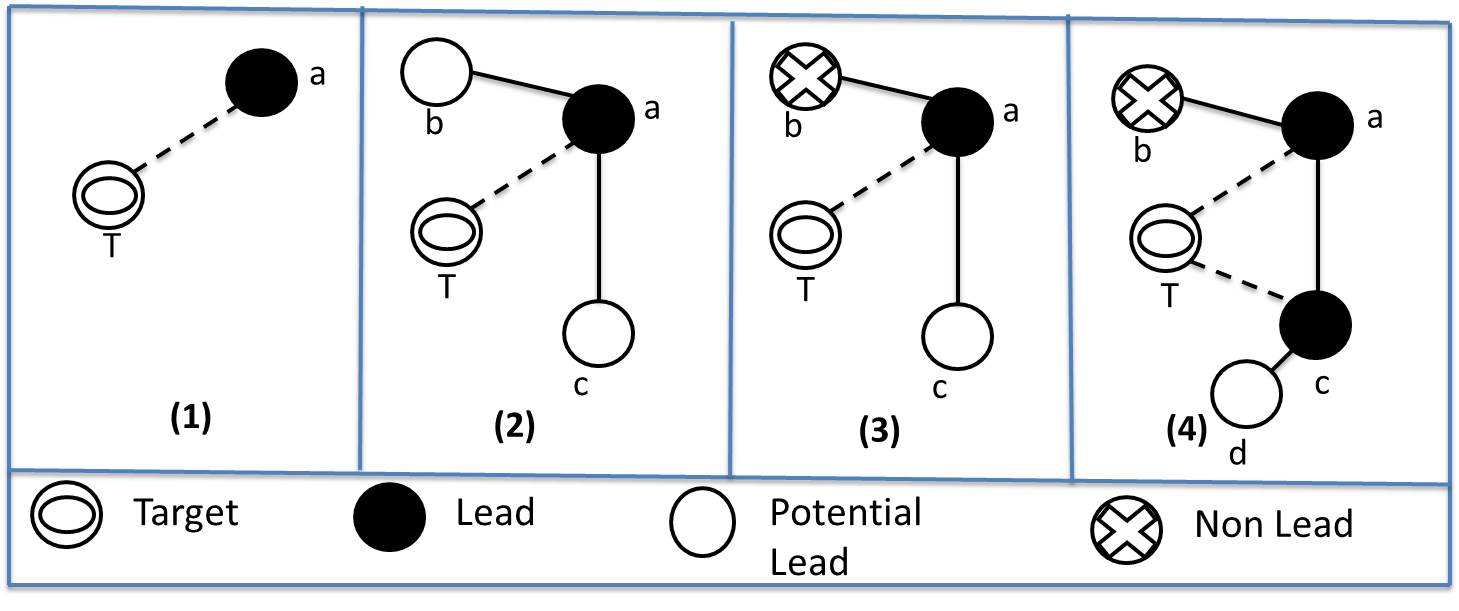
\includegraphics[width=0.8\linewidth]{btf-process-and-legend-new.jpg}
  \caption{An example of a run of Algorithm~\ref{alg:bfs}. The figure shows the CKG in the different stages}
	\label{fig:bfs_example}\label{fig:basic_fifo}
\end{figure}

% \begin{figure}[t!]
% \centering
%	 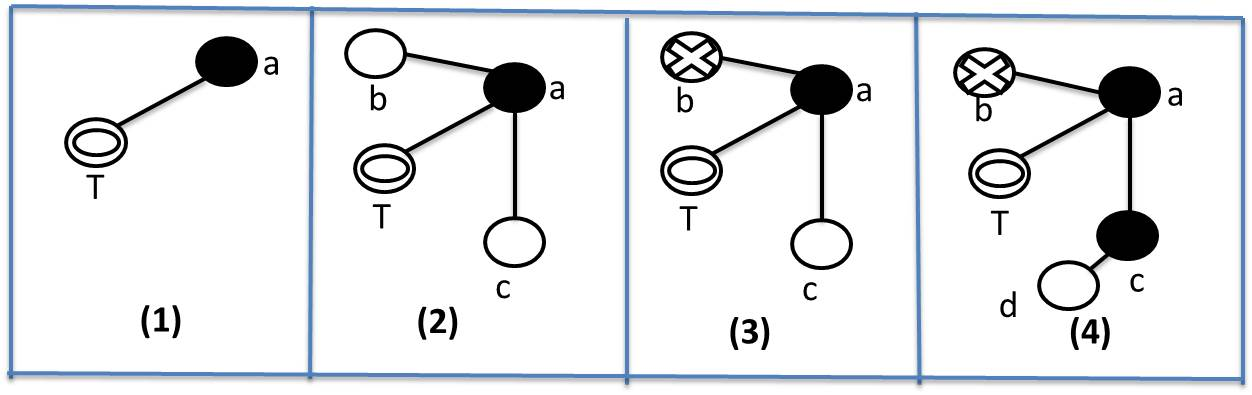
\includegraphics[width=0.7\linewidth]{basic_fifo.jpg}
%  \caption{An example the basic FIFO heuristic.}
%\end{figure} 


\section{The Restricted TONIC Framework (RTF)}
\label{sec:rtf}

One clear limitation of Algorithm~\ref{alg:bfs} is that in the worst case, it will acquire all the profiles in the OSN. This can be a serious limitation, as popular OSNs are very large. Moreover, the set of possible profiles to acquire may grow to be very large, and include many profiles that are very unlikely to be leads. Previous work showed that OSNs and social networks in general follow the homophily principle, which means that friends tend to exhibit similar attributes~\cite{mcpherson2001birds,altshuler2012security,fire2012predictingStudent}. Thus, it follows that friends of leads (i.e., profiles that appear in leads' LOFs), are more likely to be leads than randomly selected OSN profiles. 

The Restricted TONIC Framework (RTF) builds on this understanding, and focuses the search for leads by only applying the \acquire{} query to profiles that are known to be leads. Non-leads are never acquired. 
RTF may be implemented with Algorithm~\ref{alg:bfs} setting the $ChooseBest$ function to never choose a non-lead. In particle, with RTF we may simplify Algorithm~\ref{alg:bfs} --  profiles that are found to be non-lead are discarded and are not re-inserted into $OPEN$ (line~\ref{bfs:add-nl-to-open-2}). As a result, $OPEN$ only contains potential leads and lines 15--18 are redundant (they are marked with E for extended framework). 
%~\ref{bfs:expand-nl}-\ref{bfs:add-pl-to-all-2} are redundant (they are marked with E for extended framework). 
Also, a single {\em expand} action can be defined, which performs \islead{} on $best$ and acquires if it is a lead. %\note{Roni}{Last sentence is helpful or not? what motivated me in adding this is that we earlier say that expand=acquire. Thoughts? we can write everything below without mentioning the term ``expand'' but I'm not sure if this won't hurt readability}
%\note{Liron}[It's great. There is some confusion with the terms and this sentence fixes it}
 %It is important to note that for RTF (below) we never allow to acquire non-leads. Therefore, in RTF when a non-lead is added to OPEN the heuristic function will give it a very low priority and in practice it will never be chosen. The pseudocode can be further simplified for RTF as we describe below.


%In this section we present the Restricted TONIC Framework heuristics and experimental results comparing them.
 %As mentioned before, in RTF we assume that {\em friends} of leads (i.e., profiles that appear in leads' LOFs), are more likely to be leads than randomly selected OSN profiles. Therefore, we focused the search by only allowing full acquisition of {\em leads}. Meaning that each potential lead $l$ with isLead(l)=true will be acquired and its LOF(l) will be extracted and each potential lead $nl$ with isLead(nl)=false will not be acquired and its LOF(nl) will not be extracted.
 % \note{Roni}{The above is a very good and clear definition of RTF. It was missing when you talked about RTF earlier.} \note{Liron}{Moved it to the previous section}


\subsection{RTF Heuristics}

We now provide a number of heuristics for choosing which potential lead to expand next in RTF. 

A Key to the efficiency of RTF is to choose intelligently which potential lead to expand in every iteration of Algorithm~\ref{alg:bfs} (line~\ref{bfs:choose}). Next, we present several heuristics designed for this purpose. We refer to these heuristics as {\em RTF heuristics}. As a baseline RTF heuristic, consider expanding profiles in a {\em first-in-first-out} (FIFO) manner. This means that the neighbors of the initial leads are chosen first, then their neighbors and hence forth. 
Figure~\ref{fig:basic_fifo} illustrates such an expansion order. $T$ is the target profile and there is a single initial lead $a$. After profile $a$ is acquired, two profiles are discovered, $b$ and $c$. Then, they are expanded according to the order of their insertion into $OPEN$.
%Another baseline is to randomly choose which potential lead to expand next. These baselines are denoted {\em FIFO} and {\em RND}. Both baselines do not consider the topology of the OSN. \note{Roni}{Why not use the CKG, which we defined above}
Another baseline is to randomly choose the potential lead to expand next. 
These baselines are denoted {\em FIFO} and {\em RND}. Both baselines do not consider the $CKG$ (the currently known subgraph of the OSN). As the search progresses, the $CKG$ grows, containing more information about the searched OSN. By contrast, the heuristics provided next are based on analyzing the CKG in different ways.
 

%While initially only the target and the initial leads are known, more parts of the OSN topology are discovered as the search progresses. Let $V_{CKG}$ and $E_{CKG}$ be the nodes and edges of the $CKG$ (the currently known subgraph of the OSN), respectively. $V_{CKG}$ is the union of the sets $L$, $NL$ and $PL$. The following heuristics choose which potential lead to acquire by analyzing the CKG in different ways. 

% (the found leads, non-leads, and potential leads, respectively) \note{Roni}{Already defined above}
%The discovered subgraph of the OSN graph (i.e., the parts revealed when acquiring profiles) is referred to as the {\em currently known graph} \note{Roni}{Repetition of what was said above}, denoted by $CKG=(V_{CKG}, E_{CKG})$. $V_{CKG}$ is composed of three mutually exclusive sets: set of profiles found to be {\em leads} (\(L\)), the set of profiles found to be {\em non-leads} (\(NL\)), and the set of {\em potential leads} (\(PL\)). The following heuristics choose which potential lead to acquire by analyzing the CKG in different ways. \note{Roni}{Confusing. Aren't $L$, $NL$ and $PL$ maintained separately from the CKG, while here you say tha they are part of it.}

\subsubsection{Clustering Coefficient Heuristic}
Nodes in OSNs tend to form tightly connected clusters in which most people are friends of each other. This phenomenon is quantified using the notion of {\em local clustering coefficient}~\cite{clustering}. 
%The local clustering coefficient of a node in a graph is the density of edges between its neighbors. Formally, the local clustering coefficient for a node $i$ in a graph G = (V;E) with an edge $e_{ij}$ that connects vertex $v_i$ with vertex $v_j$ is: \note{Roni}{What is the difference between a vertex and a node?}
The local clustering coefficient of a node in a graph is the density of edges between its neighbors. Formally, it is the proportion of links between the nodes within its neighborhood divided by the number of links that could possibly exist between them. 
%\note{Roni}{Maybe the next sentence and formula is redundant. Thoughts?}
Let $CC(n_i)$ be the local clustering coefficient of node $n_i$, and let $N(x)$ be the neighborhood of $x$, then
\begin{equation}
CC(n_i) = \frac{2|\{e_{jk}: n_j,n_k \in N(n_i), e_{jk} \in E\}|}{|N(n_i)|(|N(n_i)|-1)}.
\end{equation}


%$k_i$ is the number of vertices, $|N_i|$, in the neighbourhood, $N_i$, of a vertex.
%The local clustering coefficient $C_i$ for a vertex $v_i$ is the proportion of links between the vertices within its neighbourhood divided by the number of %links that could possibly exist between them.

 %\note{Roni}{Consider putting here a formal definition (with the formula)}
%\note{Roni}{Now put the formula for the local clustering coefficient of $n$}
%\note{Liron}{Please review}
%\note{Roni}{some inconsistencies which I fixed. $k$ is used twice (first as a variable in the set, second as $k_i=|N_i|$). Unclear usage of node vs. vertex. }

A profile connected to a cluster of leads is likely to be part of that cluster and thus likely to also be a lead. 
An intuitive example of such a case is a small university department where a member of that department is the target. It seems reasonable that members of that department form a dense cluster in the OSN and are likely to be leads. Therefore, as more leads are found in that cluster, profiles in it will have higher local clustering coefficient and it would be worthwhile to expand them.
%because they would be more %likely to be leads. \note{Roni}{Not sure if this is convincing}

%university cluster is found, it would be easier to reach other leads in that cluster since they are probably connected to the lead found. \note{Roni}{Elaborate more. Why does this example show that the local clustering coefficient would be a good heuristic?}
%\note{Liron}{I added an explanation - please review it}

Building on this intuition we propose a heuristic that is based on computing the local clustering coefficient (CC) of each of the potential leads and choosing to expand the potential lead with the highest CC. 
More formally, let $L(pl)$ be the set of leads that are friends of the potential lead $pl$ in the CKG. The CC of $pl$ in the CKG is the number of links between $L(pl)$ divided by the number of possible links among $L(pl)$ :
\begin{equation}
CC(pl)=\frac{2\cdot\left|\left\{(u,v)\in E_{CKG} | u,v\in L(pl)\right\}\right|}{|L(pl)|\cdot(|L(pl)|-1)}
\end{equation}
In RTF, the neighborhood of a potential lead consists of only the previously acquired leads. Thus $L(pl)=N(pl)$ and the above formula is exactly the local clustering coefficient given earlier. The {\em CC heuristic} is the heuristic that chooses to expand the potential lead with the highest CC. 
% For example, a potential lead $pl$ will have a $CC$ of one if all its lead friends form a clique. 


\begin{figure}
\centering
\begin{subfigure}{.39\textwidth}
\centering
  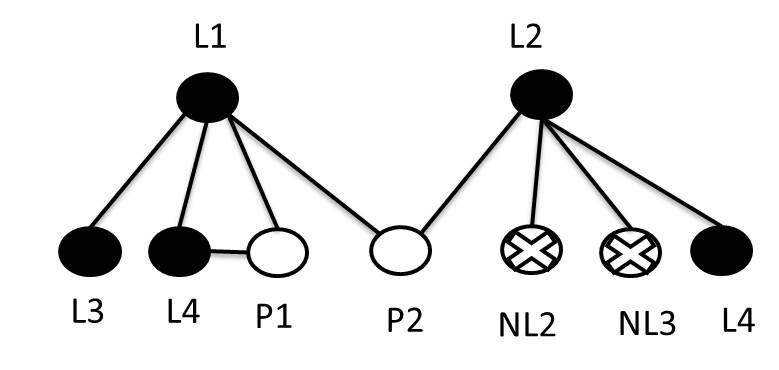
\includegraphics[width=\linewidth]{cc.jpg}\\
   \caption{CC}\label{fig:cc}
\end{subfigure}
\begin{subfigure}{.39\textwidth}
\centering
  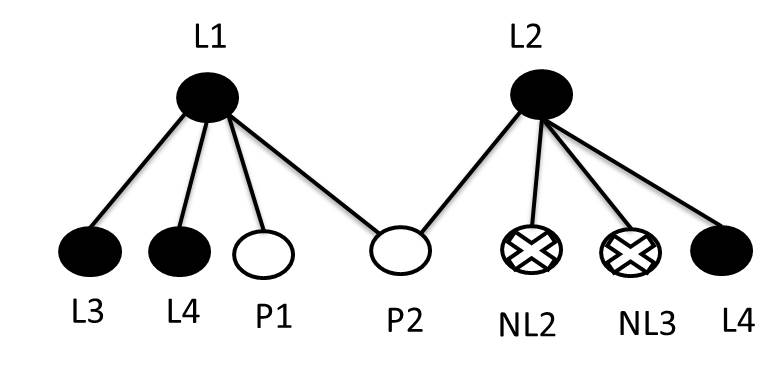
\includegraphics[width=\linewidth]{KD_NEW.jpg}\\
   \caption{KD}\label{fig:kd}
\end{subfigure}
\begin{subfigure}{.19\textwidth}
  \centering
  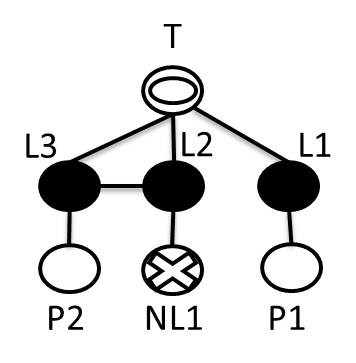
\includegraphics[width=\linewidth]{FM_BTF.jpg}\\
   \caption{FM}\label{fig:fm_btf}
\end{subfigure}
\caption{Examples of RTF heuristics.} 
\end{figure}


An example of CC heuristic is provided in Figure~\ref{fig:cc}. White nodes are potential leads, black nodes are leads, and white nodes with X are non-leads.
$CC(P1)=1$, since the number of links between $L(P1)$ is 1 (the link between L1 and L4) out of one possible link among $L(P1)$.
$CC(P2)=0$, since there are no links between $L(P2)$. Thus, the CC  heuristic will choose to expand node $P1$ before node $P2$.

\subsubsection{Known-Degree Heuristic}
The CC heuristic ignores the number of friends that a potential lead has. In fact, potential leads with a single friend will have the highest CC score (one). This is a disadvantage of CC, because it has been shown that degree of nodes in a social networks exhibits a power-law distribution~\cite{barabasi1999emergence}, and previous work has shown that an effective strategy for searching in such graphs is to direct the search towards nodes with a high degree~\cite{adamic2001searchInPowerLaw}. 
%\note{Roni}{Rami -- should the relevant network characteristic here be ``preferential attachment'' and not ``power law''? }
%\note{Liron{{Because of the preferential attachment, it creates a power law network in which many profiles have a small number of friends and a few profiles have a large number of friends}
The intuition behind this is that high degree nodes are connected to many other nodes, and thus are better sources for searching than low degree nodes.


Identifying the potential lead with the highest degree, or is connected to the most leads, is not possible in TONIC, since the problem solver does not know the true degree of potential leads before they are acquired. However, the degree of a potential lead in the CKG {\em is} known. This is called the {\em known degree} (KD) of a node and the corresponding heuristic, denoted as the {\em KD heuristic}, expands nodes in the order of their KD. This heuristic was previously used to find cliques in unknown graphs~\cite{stern2012findingPatterns}. In RTF, the KD of a potential lead $pl$ is the number of acquired leads that are friends of $pl$ (denoted earlier as $L(pl)$), since only leads are acquired. An example of KD is provided in Figure~\ref{fig:kd}.
$KD(P1)=1$ (connected to $L1$) while $KD(P2)=2$ (connected to $L1$ and $L2$). Thus, the KD  heuristic will choose to expand node $P2$ before node $P1$.


\subsubsection{Promising-Leads Heuristics}
\label{sec:promising}

The KD heuristic expands potential leads according to the number of acquired leads that are connected to them. This is reasonable if all leads have an equivalent effect on the likelihood that a potential lead connected to them is a lead.
%Liron: Rami, Ariel, Roni - please review this sentence. I am not sure about it's ending
% Roni: not perfect but I do not have a good alternative. Can keep it as is in my view.
Consider the example presented in Fig~\ref{fig:PromiseMotivation}. P1 and P2 are potential leads, both connected to one lead. P1 is connected to a lead with 3 lead friends while P2 is connected to a lead with 3 non lead friends. 
We believe that P1 is more likely to be a lead than P2 since it is connected to a more ``promising'' lead.
 Following, we explore an alternative approach that considers not just the amount of leads that a potential lead is connected to, as the KD heuristic, but also how ``promising'' these leads are %\note{Roni}{Minor: in Latex, instead of using "bla bla", use ``bla bla''. It looks differently in the output and some reviewers are nudnikim. Please fix throughout the paper.},\note{Liron}{Done} 
 in the sense that potential leads connected to them are more likely to be leads. 

\begin{figure}
\centering
\begin{subfigure}{0.35\linewidth}
  \centering
  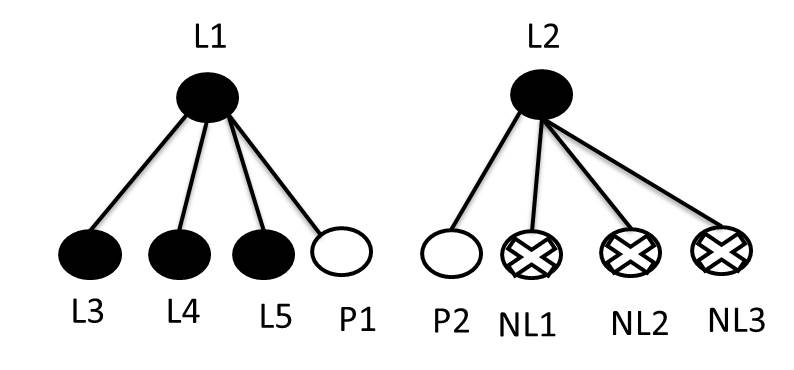
\includegraphics[width=\linewidth]{PromiseMotivation.jpg}
   \caption{Motivation.}\label{fig:PromiseMotivation}
\end{subfigure}
\begin{subfigure}{0.55\linewidth}
  \centering
  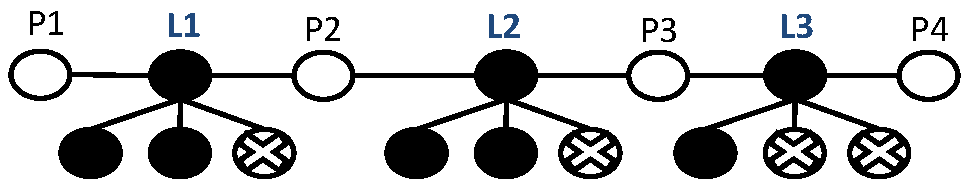
\includegraphics[width=\linewidth]{bysp-good_cropped.pdf}
   \caption{Example.}\label{fig:Promising}
\end{subfigure}
\caption{The Promising Heuristic.}
\end{figure}

The first step in creating such a heuristic is to define a measure of how ``promising'' a lead is. An ideal ``promising'' measure for a lead $m$ would be the probability that a randomly drawn generated neighbor of $m$ is a lead. This is the ratio of potential leads connected to $m$ that are leads. We denote this ideal promising measure as $pm^*(m)$.

Unfortunately, $pm^*(m)$ cannot be known before {\em all} neighbors of $m$ are acquired. As a practical alternative, we consider the ratio of leads among the {\em expanded} neighbors of $m$. Formally, we divided the LOF of an expanded lead $m$ into three sets: leads, non-leads and potential leads, denoted as $L(m)$, $NL(m)$ and $PL(m)$, respectively. The promising measure we propose, called the {\em promising factor} and denoted by $\pf()$, is computed by $\pf(m)=\frac{L(m)}{L(m)+NL(m)}$.\footnote{Initially, it is possible that $L(m)+NL(m)=0$, making $\pf(m)$ undefined. To avoid this, we set $\pf(m)=0.5$ in this case.}


\subsubsection{Aggregating Promising Leads}

If every potential lead was connected to a single expanded lead, then a straightforward TONIC heuristic that considers the promising factor would expand the potential lead that is a friend of the expanded lead with the highest promising factor. However, a potential lead may be connected to a set of expanded leads, each having a different promising factor.
%Next, we propose several TONIC heuristics that use different ways to consider the promising factor of all the leads in $L(pl)$.

%\subsubsection{Simple Aggregations} 
Two simple ways to aggregate the promising factors of the leads is to take their maximum or their average. We call the corresponding TONIC heuristics $MaxP$ and $AvgP$, respectively. Formally, $MaxP$ chooses to expand the potential lead $pl$ that maximizes $\max_{m\in L(pl)}{\pf(m)}$, while $AvgP$ chooses to expand the potential lead $pl$ that maximizes $\frac{1}{|L(pl)|}\sum_{m\in L(pl)} \pf(m)$. 

%[[R 1.20]]
As an example of these aggregation methods, consider again the graph in Figure~\ref{fig:Promising}. 
There are four potential leads, $P1$, $P2$, $P3$, and $P4$, and three leads $L1$, $L2$, and $L3$. 
The promising factor of leads $L1$, $L2$, and $L3$ is $\frac{2}{3}$, $\frac{2}{3}$, and 
$\frac{1}{3}$, respectively. 
The $MaxP$ values for potential leads $P1$, $P2$, $P3$, and $P4$, are $\frac{2}{3}$, $\frac{2}{3}$, $\frac{2}{3}$, and $\frac{1}{3}$, respectively, while the $AvgP$ values for these potential leads are $\frac{2}{3}$, $\frac{2}{3}$, $\frac{1}{2}$, and $\frac{1}{3}$. Thus, using $MaxP$ will result in choosing first one of the potential leads $P1$, $P2$, and $P3$ (but not $P4$, which has a smaller $MaxP$ of $\frac{1}{3}$). In contrast, using $AvgP$ will not allow choosing $P3$ first, and either $P1$ or $P2$ will be expanded first (since both have $AvgP$ of $\frac{2}{3}$ while $P3$ and $P4$ have an $AvgP$ of $\frac{1}{2}$ and $\frac{1}{3}$, respectively. 

%According to the $MaxP$ heuristic  $MaxP(P1)=\frac{2}{3}$, $MaxP(P2)=\frac{2}{3}$,and $MaxP(P3)=\frac{2}{3}$. 
%Thus, according to the MaxP heuristic all three potential leads are equally preferable, and one may choose arbitrarily which be expanded first (e.g., by breaking ties randomly). 
%According to the $AvgP$ heuristic, $AvgP(P1)=1$,  $AvgP(P2)=1$, and $AvgP(P3)=1$.   and $AvgP(P2)=\frac{1}{3}$. Thus, in P1 is expanded first also according to the $AvgP$ heuristic.



%There are two potential leads, $P1$ and $P2$. The only lead connected to $P1$ is $L1$, which has $\pf(L1)=\frac{3}{3}=1$. $PL2$ is connected to two leads, $L2$ and $L3$, with $\pf(L2)=\pf(L3)=\frac{1}{3}$.
%According to the $MaxP$ heuristic, $MaxP(P1)=1$ and $MaxP(P2)=\frac{1}{3}$. Thus, P1 will be expanded first. According to the $AvgP$ heuristic, $AvgP(P1)=1$ and $AvgP(P2)=\frac{1}{3}$. Thus, in P1 is expanded first also according to the $AvgP$ heuristic.


$MaxP$ only considers the lead that is most promising, and ignores all the other leads in $L(pl)$. $AvgP$ takes into consideration all the leads in $L(pl)$ but may diminish the effect of a very promising lead in $L(pl)$, if $L(pl)$ contains other less promising leads. Next, we consider a more sophisticated way to aggregate the promising factors of the leads.




\subsubsection{Bayesian Aggregation}
The promising factor $pf(m)$ is designed to estimate $pm^*(m)$, which is the probability that a potential lead connected to $m$ is a lead. 
We therefore propose another way to aggregate the promising factors that is based on a Na\"{\i}ve Bayes approach to aggregate probabilities.
\begin{equation}
\displaystyle BysP(pl)=1-\prod_{m\in L(pl)}(1-pf(m)) 
\end{equation}

\noindent The TONIC heuristic that chooses to expand the potential lead $pl$ with the highest $BysP(pl)$ is denoted as the {\em Bayesian Promising} heuristic, or simply $BysP$. $BysP$ has the following desirable attributes. Unlike the $AvgP$, discovering a new lead $m$ that is connected to $pl$ is guaranteed to increase (or at least not decrease) $BysP(pl)$, since $pf(m)\leq 1$. Unlike $MaxP$, any change in the promising factor of each of the leads in $L(pl)$ affects the $BysP(pl)$: it will increase or decrease according to the increase or decrease of the promising factor of the leads in $L(pl)$.


%[[R 1.20]]
As an example of the Bayesian Promising heuristic, consider again the graph in Figure~\ref{fig:Promising}. 
%Figure~\ref{fig:promising_new}. 
The $BysP$ values of the four potential leads are $BysP(P1)=1-(1-pf(L1))=\frac{2}{3}$, 
$BysP(P2)=1-(1-pf(L1))\cdot(1-pf(L2))=\frac{8}{9}$, 
$BysP(P3)=1-(1-pf(L2))\cdot(1-pf(L3))=\frac{7}{9}$, and $BysP(P4)=1-(1-pf(L4))=\frac{1}{3}$. 
Thus, $BysP$ will choose to expand first $P2$. 
In contrast, both $AvgP$ and $MaxP$ may expand some other potential lead first ($P1$ for $AvgP$ and $P1$ or $P3$ for $MaxP$). 

%As mentioned earlier, there are two potential leads, $P1$ and $P2$. The only lead connected to $P1$ is $L1$, which has $pf(L1)=\frac{3}{3}=1$. $P2$ is connected to two leads, $L2$ and $L3$, with $pf(L2)=pf(L3)=\frac{1}{3}$.
%Thus $BysP(P1)=1-(1-pf(L1))=1$. $BysP(P2)=1-(1-pf(L2))(1-pf(L3))=\frac{5}{9}$. Therefore, according to the $BysP$ heuristic $P1$ will be expanded first.



\subsubsection{Friends Measure Heuristic (FM)}
\label{sec:friendsMeasure}

% Link prediction algorithms can be used to do TONIC
The TONIC problem bears some resemblance to the \emph{link prediction} problem \cite{liben2007link}, where the goal is to predict whether two profiles are connected (see Section~\ref{sec:relatedWork} for more details). Link prediction algorithms return the likelihood of a link to exist between two profiles. This suggests the possibility of employing a link prediction algorithms for TONIC, by ranking nodes in $OPEN$ according to the likelihood of a link to exist between a node and \target .\footnote{A more comprehensive discussion on the relation between link prediction and TONIC is given in Section~\ref{sec:relatedWork}.} In fact, a notion very similar to KD was extensively used in link-prediction research, where it is known as the common-friend concept~\cite{liben2007link}. Simply put, we expect a potential lead that has many friends that are leads to also be a lead.


% We tried FM
The \emph{Friends Measure} is a very successful link prediction method that estimates the likelihood of a connection between two profiles by counting the number of common friends and the number of links between the friends of the two profiles~\cite{fire2013linkPrediction}.
Formally, the friends measure ($fm$) between profiles two profiles ($u$ and $v$) is defined as follows:
\begin{equation}
fm(u,v)= \sum\limits_{x\in N(u)}~~\sum\limits_{y \in N(v)} \delta(x,y)
\end{equation}

\begin{equation}
\delta(x,y) = \begin{cases}
1 &\text{if $x=y$ or $(x,y)\in E$ or $(y,x) \in E$}\\
0 &\text{Otherwise}
\end{cases}
\end{equation}
% [R 1.21]
We note that the Friends Measure is a special case of the Katz measure~\cite{katz1953aNewStatus} in undirected graphs, and is somewhat similar to the well-known Jaccard's coefficient~\cite{fire2014computationallyEfficient}. 
%Jaccard's coefficient of two nodes is the ratio between the intersection of the nodes' neighborhoods and the union of their neighborhoods. 
In RTF, we are interested to predict if a given potential lead $pl$ has a link to $target$ (i.e., to predict if $pl$ is a lead). Computing $fm(pl,\target)$ requires knowing the neighborhood of $pl$ and $\target$ ($N(pl)$ and $N(\target)$, respectively). $N(pl)$ is not known before $pl$ is acquired and $N(\target)$ is also unknown, otherwise we would know all the leads. Instead, we use the neighborhoods of $pl$ and $\target$ in the CKG. As only leads are acquired in RTF, $N(pl)$ in the CKG is exactly $L(pl)$. Since we assume that leads are all neighbors of $\target$, then $N(target)$ in the CKG is simply the set of known leads ($L$). Thus, the resulting Friends Measure of $pl$ and $target$ is:
\begin{equation}
fm(pl,target)= \sum\limits_{x\in L}~~\sum\limits_{y\in L(pl)  } \delta(x,y)
\end{equation}
%\note{Roni}{Liron/Rami -- please verify the above}
%\noindent where  $\delta(x,y)$ is defined as before and L represent all the Leads in the CKG.
%x represent the target's neighborhood, which contains only leads (every profile connected to the target is considered a lead) and y represent $p$'s neighborhood. Since in RTF, a profile can only have lead friends, $y$ represents the leads connected to $p$.
\noindent The heuristic that chooses to expand the potential lead $pl$ the highest $fm(pl,\target)$ is called {\em FM}. 




Figure~\ref{fig:fm_btf} provides an example of the FM heuristic. P1 and P2 are two potential leads, and $\target$ is denoted by $T$. P1 has one mutual friend with the target (L1) and therefore $fm(P1,T)=1$. In contrast, P2 also has one mutual friend with the target (L3), however the target's neighborhood and P2's neighborhood's contain and additional mutual friend (L2) and therefore $fm(P2,T)=2$
Therefore, the FM  heuristic will choose to expand node $P2$ before node $P1$.


%In a sequel~\cite{bnaya2013social-journal} we have evaluated a general technique, based on a unique variant of the Multi-Arm Bandit problem. The technique was applied to TONIC and to the problem of finding communities in an OSN. Importantly, the goal of the MAB based approach was a search method that is not based on a domain-specific heuristic such as the BysP or FM. Thus, we mention it here for completeness, but have not evaluated it experimentally. 
%Experimentally, their results were comparable to BysP, and they did not consider ETF at all. 



\subsection{Experimental Results}
\label{sec:btf-experimentalResults}
Next, we evaluate the performance of the different RTF heuristics. Most experimental results presented in this paper are on the Google+, but Section~\ref{sec:otherNetworks} presents highlights from our research on other other OSNs. Google+ is one of the largest social networks, having more than 540M registered users and 300M users that are active monthly (according to Wikipedia). 

%\note{Roni}{There is still a problem here. The definition of islead in the prob. def. is different. As I suggested above, I think this definition should be given above in the prob. def. section, and then you don't need to write all this here.} \note{Liron}{Changed it in the beginning and deleted it from this section}\note{Roni}{Good}


%\subsubsection{Data Collection}
%\begin{figure}%[t]
%\centering
%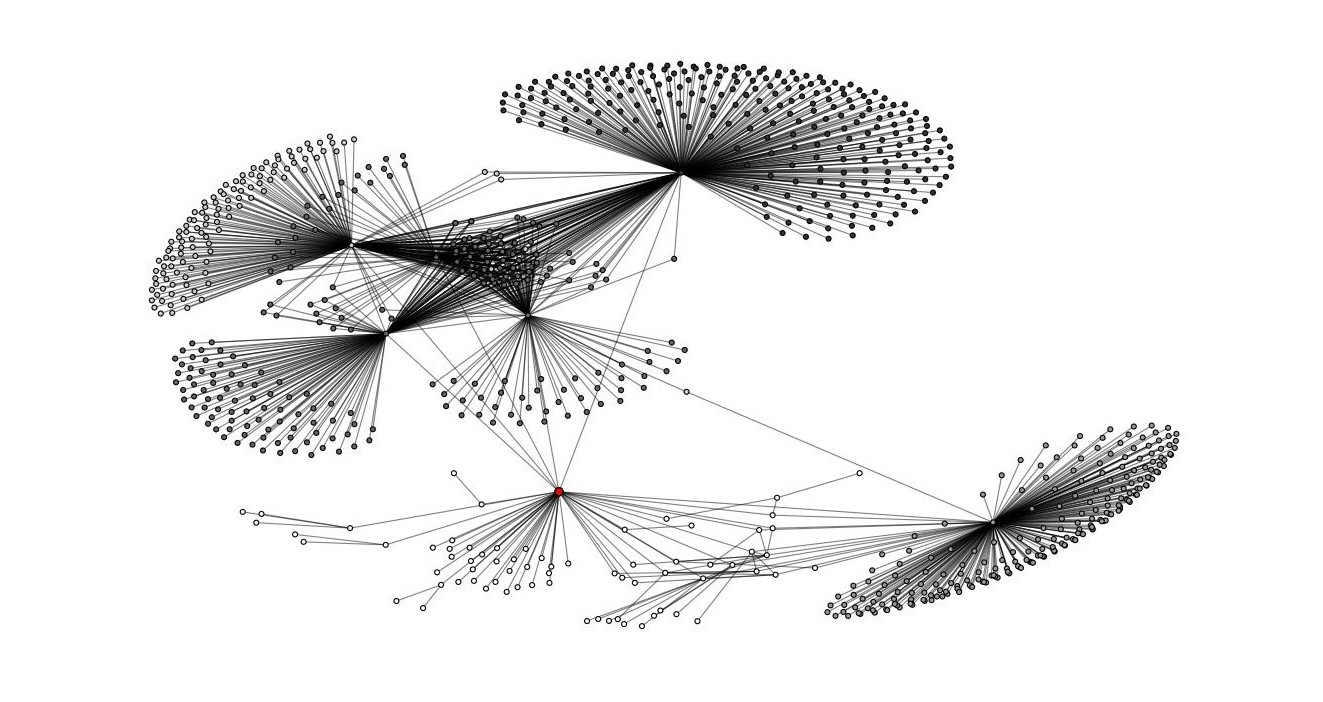
\includegraphics[width=0.7\linewidth]{figure_sample_target_BTF.JPG}
%\caption{Sample network of the RTF relevant neighborhood of a target.}
%\label{fig:net}
%\end{figure}

The data set used in our experiments was obtained from the Google+ network and included 211K profiles with 1.5M links between them. This data set was collected by Fire et. al \cite{fire2011linkPrediction} and made available at \url{http://proj.ise.bgu.ac.il/sns/datasets.html}. From this data set we randomly selected  a set of 100 profiles having at least 30 friends. These profiles were used as the targets in our experiments. 


Since in RTF only potential leads can be acquired, the $CKG$ for each target can contain at most the set of leads and their neighbors throughout the search. We call these set of profiles the {\em relevant neighborhood} of the target. In our data set, the size of relevant neighborhood ranged from 233 to more than 4,000 profiles. 
%Figure \ref{fig:net} presents the relevant neighborhood in RTF of one of the targets in our data set.
%\note{Roni}{Ok, the above is not consistent with current definitions.} \note{Liron}{fixed}

The search for leads for each target was executed using RTF using the following heuristics: RND, FIFO, CC, KD, AvgP, MaxP, BysP, and FM. Three friends of every target were randomly chosen as the initial leads. The search continued until {\em all} potential leads were expanded.

%\note{Roni}{A big plus to the paper would be to say here that the data is availabe online in some website. Can we do that?} \note{Liron}{I added a link to mickey's datasets website - is this ok? can we do that? (copyrights etc))?}\note{Roni}{This is perfect.}
 
 
\begin{figure}%[t]
\centering
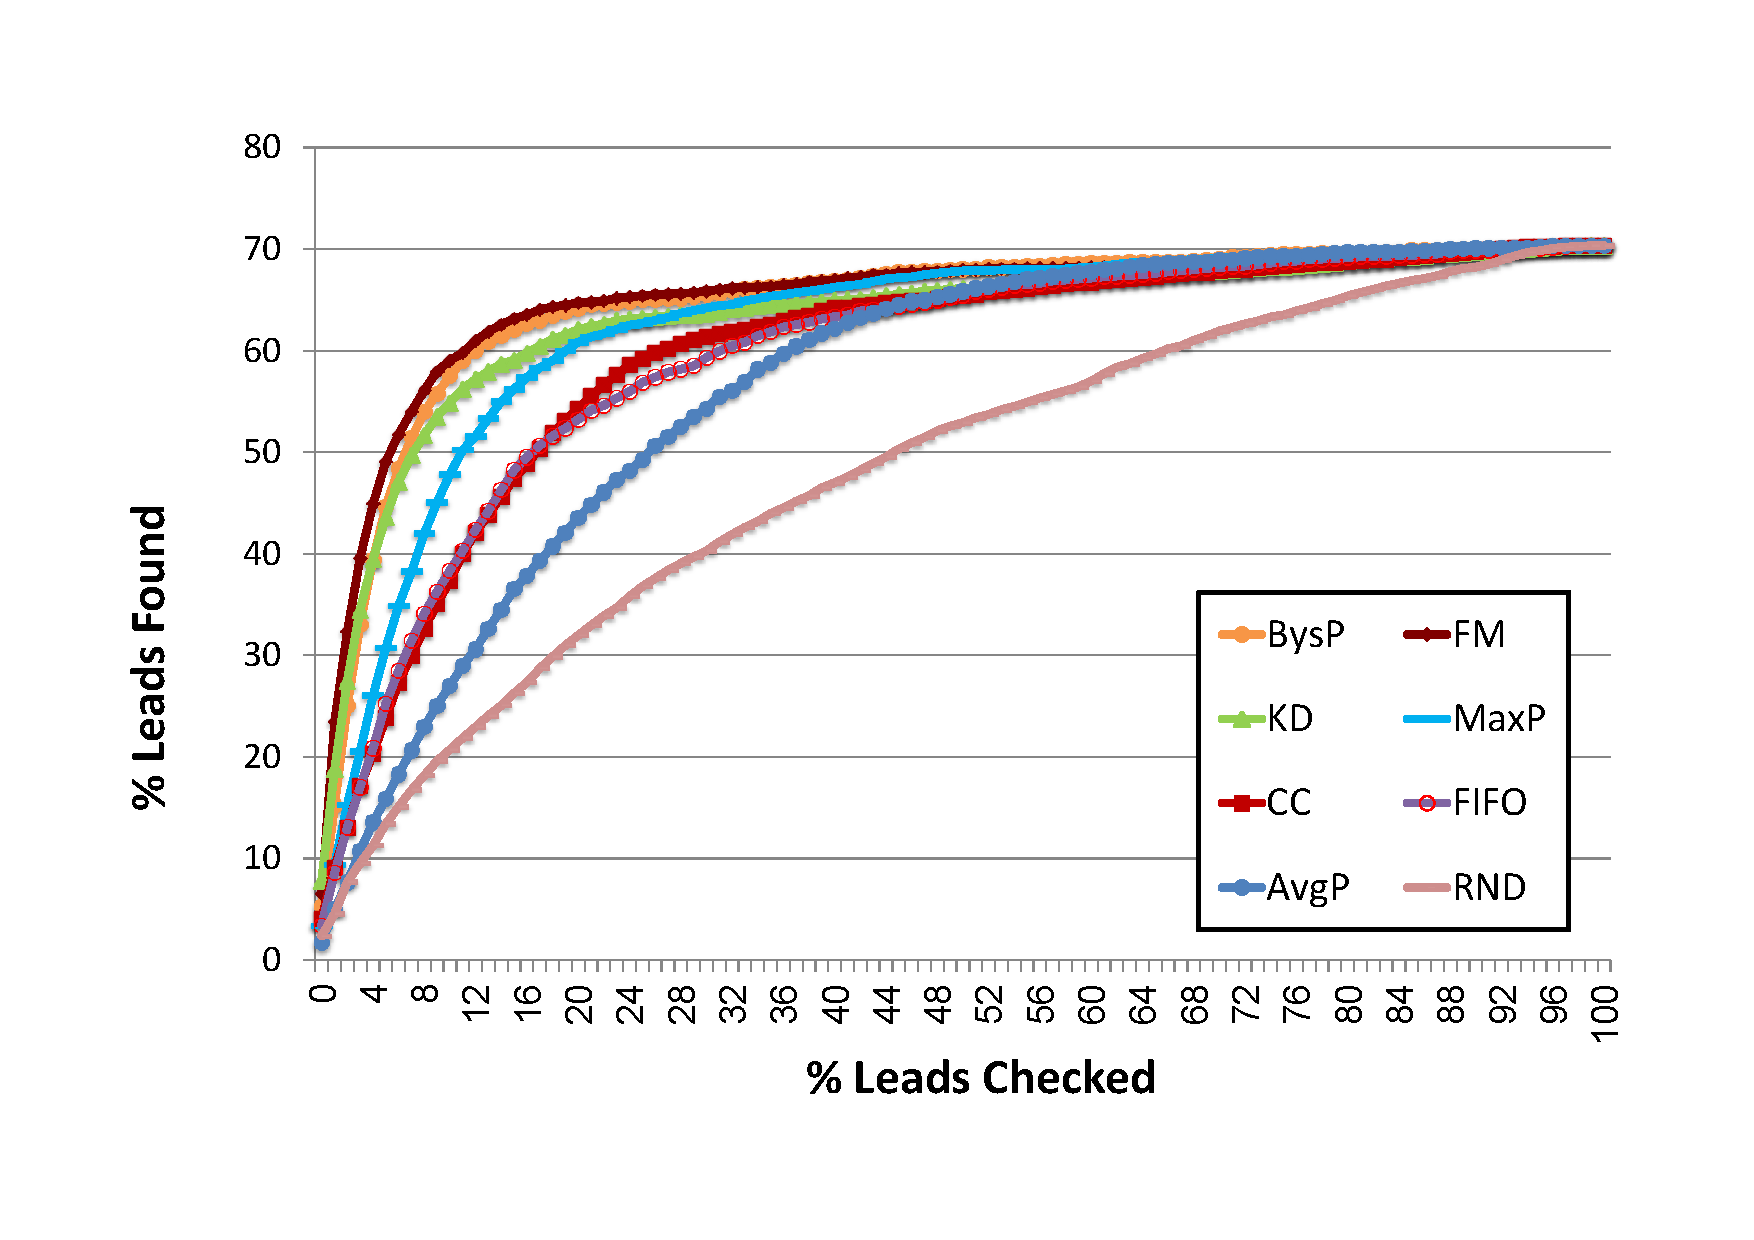
\includegraphics[width=0.5\linewidth,  trim={2.0cm 2.5cm 2.5cm 2.0cm},clip]{BTF_all.pdf}
\caption{\% of leads found vs. \% of potential leads checked.}
\label{fig:checkedVsFound}
\end{figure}
Figure~\ref{fig:checkedVsFound} analyzes the performance of the different RTF heuristics
for the anytime objective function (Definition~\ref{def:budget}). 
%Note that all performed queries are counted in the budget. However, since the purpose of TONIC is to acquire leads, we focused the presentation of our results on the budget consumption that does not directly acquiring leads. In other words, we only count \islead{} queries of potential leads and \acquire{} queries for non-leads. We refer to this count as the number of ``iterations'' as it corresponds to the number of iterations of Algorithm~\ref{alg:bfs}. 



The $x$-axis of Figure~\ref{fig:checkedVsFound} is the  percentage of potential leads queried so far (by \islead{}) out of the total number of potential leads reachable from the initial leads. The $y$-axis represents the fraction of leads found out of all existing leads, averaged over all the 100 targets in our data set. Note that since RTF limits the search to only acquire leads, not all leads are reachable from the initial leads, and thus the $y$-axis does not reach 100\% even after all potential leads are checked. 

%shows the following analysis. 
%The $x$-axis represents the percentage of RTF iterations preformed (percentage from the total number of potential-lead reachable from the initial leads), where each iteration represents an \islead{} query and if necessary, an \acquire{} query as well. The $y$-axis represents the fraction of leads found out of all existing leads, averaged over all the 100 targets in our data set. Note that since RTF limits the search to only acquire leads, not all leads are reachable from the initial leads, and thus the $y$-axis does not reach 100\% even after all potential leads are checked. 


%[[AFCOMMENT: I do not like the above paragraphs]]
The result in Figure~\ref{fig:checkedVsFound} show that KD, FM and BysP are able to find more leads earlier during the search process and in general outperform all other heuristics. In particular, BysP and FM dominate all other heuristics. %, and BysP has a slight advantage of FM. 
%\note{Liron}{Should i still say the bysp dominates all other heuristics? bysp and fm are extremely close (avg 64.433 vs 64.292 respectively}
%\note{Roni}{Rewrote to say that BysP and FM are the winners. Liron -- can you check statistical significance in each time step? the numbers above - 64.433 and 64.292 are averages over the entire x-axis, where they looks pretty much the same, but maybe in some time steps the difference is statistically significant}
%\note{Liron}{I did a tTest on the rows in pivot table  (between EbysP and FM) and got 0.000026 . Meaning, significant}.


\section{Extended TONIC Framework (ETF)}
\label{sec:etf}



As seen in the results above, RTF may miss 30\% of the leads. These 30\% of leads are not reachable from the set of initial leads by a path which contains leads only. In this section, we relax the restriction imposed by RTF, allowing non-leads to be acquired. We refer to this TONIC framework as the Extended TONIC Framework (ETF). The scope of the search in ETF is larger than RTF, enabling reaching a larger set of profiles and potentially finding more leads. % (second degree friends of leads as oppose to only first degree friends in RTF). 


To prevent the search from scattering, ETF limits the non leads that may be acquired to profiles that are at most $n$ edges in the CKG from a known lead, where $n$ is a parameter. ETF($n$) denotes ETF with this parameter. Thus, RTF is actually ETF(0), since only leads are acquired, while running Algorithm~\ref{alg:bfs} unrestricted is in fact ETF($\infty$). 

%%%%%%%%%%%%%%%%%%%%%%%%%%%%%%%%%%%%%%%%%%%%%%%%%%5
\subsection{Reachable Leads in ETF}
%--------------------------------------------------
The choice of the $n$ parameter in ETF affects the number of leads that can be reached. Another factor that affects the number of reachable leads is the number of initial leads. 
Increasing both parameters ($n$ and the number of initial leads) is expected to increase the number of reachable leads. This is demonstrated in Table~\ref{tab:tiers}, which shows the average percentage of reachable leads as a function of these parameters (averaged over all the targets in our data set). We use the term {\em tier} to refer to the set of profiles that are reachable with ETF($n$) for a given number of initial leads.
The table columns represent the number of tiers used, and the rows are the number of initial leads (rows). Note that since the initial leads are expected to be very hard to obtain (e.g., obtained via manual labor), we focused our analysis on a relatively small numbers of initial leads.

%Note that since the initial leads are expected to be very hard to obtain (e.g., obtained via manual labor), we focused on small numbers of initial leads. 

First, consider the impact of the number of initial leads. 
From a single initial lead the TONIC process can reach a significant fraction of all leads (more than 60\% in all cases). 
Every additional initial lead increases the fraction of reachable leads. 
The second initial lead increases the fraction of reachable leads by a margin of 6.6\% in tier 0 and approximately 4\% in higher tiers. 
This margin decreases with each additional initial lead, and we observe only a marginal advantage for adding more than 3 initial leads. 
As an operational guideline we suggest obtaining initial leads with different kinds of acquaintances with the target. For example, one family member, one co-worker, and one blog fan. 


With every additional tier the number of profiles in the corresponding tier grows, and the search will be able to reach more leads. The results in Table~\ref{tab:tiers} show this trend very clearly. The percentage of reachable leads increases significantly when considering also profiles from tier 1. For example, with 3 initial leads 70.51\% leads are reachable in tier 0, while an additional 17\% of the leads become reachable by considering tier 1 profiles too. Thus, in \(ETF(1)\) we can find more leads than in \(RTF\). However there is not much difference between the number of leads found in higher tiers (tier 2 and 3). Therefore we focus in the rest of this paper on ETF(1). 


%However, larger tiers have also more non-leads, causing potential waste in querying them. To provide insight into how to choose $n$ intelligently, Table~\ref{tab:BTFtiers} shows the average percentage of leads reachable in each tier from a certain number of initial leads. As can be seen, the exploration of tier 1 profiles can increase the number of leads found substantially compared to tier 0, i.e., in \(ETF(1)\) we can find more leads than in \(RTF\). However there is not much difference between the number of leads found in higher tiers (tier 2 and 3). Therefore we focus in the rest of this paper on ETF(1). 


%Adding initial leads increases the average number of reachable leads because people tend to be connected to a few social cycles (a.k.a communities) of friends in OSNs. \note{Roni}{This seems very obvious to me}
%In some cases a few links may exist between peoples in different social cycles while in other cases the target can be the only relation between them. In the latter cases, TONIC process starting from initial leads located only within one such social cycle cannot reach leads located in the others. Increasing the number of initial leads increases the number of social cycles that can be explored by the TONIC process. 


%It is also important to note that, the margin due additional initial leads is higher in \(RTF\) than in \(ETF\). 


%TONIC receives as input a small set of initial leads from which the search begins.  As described earlier, obtaining these initial leads may be very costly. However, the set of leads reachable increases as more initial leads are given, thus potentially leading to more leads found and higher net gain.  For a given target and initial leads, ETF partitions the OSN to {\em tiers}, where tier $n$ is the profiles that can be acquired by ETF($n$). 

%Next, we examine the effect of the number of initial leads on the percentage of reachable leads in various tiers. 
%Note that since the initial leads are very hard to obtain, we focus on small numbers of initial leads. 

% Thus, the impact of adding initial leads is more pronounced in RTF (tier 0), while it is relatively small for ETF(1) and higher tiers. 
% For example, the results suggest that unlike RTF, for ETF(1) or higher there is no need for more than three initial leads, as the added \% of leads does not increase significantly.

 


%As $n$ increases, the number of profiles in the corresponding tier grows, and the search will be able to reach more leads. However, larger tiers have also more non-leads, causing potential waste in querying them. To provide insight into how to choose $n$ intelligently, Table~\ref{tab:BTFtiers} shows the average percentage of leads reachable in each tier from a certain number of initial leads. As can be seen, the exploration of tier 1 profiles can increase the number of leads found substantially compared to tier 0, i.e., in \(ETF(1)\) we can find more leads than in \(RTF\). However there is not much difference between the number of leads found in higher tiers (tier 2 and 3). Therefore we focus in the rest of this paper on ETF(1). 


\begin{table}[t!]
\centering
\begin{tabular}{c | c| c |c| c }

			  & \multicolumn{4}{|c}{Tiers}\\
Initial leads & 0 & 1 & 2 & 3 \\
\hline
1 & 61.34\% & 82.78\% & 82.78\% & 83.10\%\\
2 & 67.94\% & 86.75\% & 86.75\% & 87.07\%\\
3 & 70.51\% & 88.28\% & 88.28\% & 88.60\%\\
4 & 72.19\% & 88.52\% & 88.52\% & 88.84\%\\
5 & 73.81\% & 88.82\% & 88.82\% & 89.11\%\\

\end{tabular}%\vspace{-0.3cm}
\caption{\label{tab:tiers}\label{tab:BTFtiers}\% of leads reachable in different tiers from different numbers of initial leads. Note that tier 0 is actually BTF. %[[R1.22]]
%
}%
\end{table}

%\note{Roni}{We will probably be asked how the number of initial leads impacted the actual search, not just the number of reachable leads}
%\note{Liron}{added the following:}
% We have also compared the performance of the proposed heuristics in terms of DCG as a function of the number of initial
% leads. Naturally, the DCG increases with the number of initial leads, as the first profiles acquired are the initial leads, which are guaranteed to be leads. In addition, the same trends as shown in results section were kept.



\subsection{ETF Heuristics}
A key difference between RTF and ETF is that $OPEN$ in RTF contained only potential leads while in ETF $OPEN$ can also contain non-leads. This is because in RTF a potential lead found to be a non-lead is discarded, while in ETF($n$) discovered non-leads are re-inserted into $OPEN$. These re-inserted profiles are later considered for expansion if they are not too far from a known lead (where ``too far'' is with respect to the $n$ parameter). % (lines~\ref{expand:add-nl-to-open-1}, \ref{expand:add-nl-to-open-2},  and~\ref{expand:add-nl-to-open-3})$d_L(\cdot)\leq n$ (lines~\ref{expand:expand-nl-1}--\ref{expand:expand-nl-2}).
Note that the distance of non-leads to known leads can change as the search progresses and new leads are discovered.

\begin{figure}[t!]

  \centering
  % Requires \usepackage{graphicx}
 % \includegraphics[width=\linewidth]{process-and-legend-2.jpg}\\
	 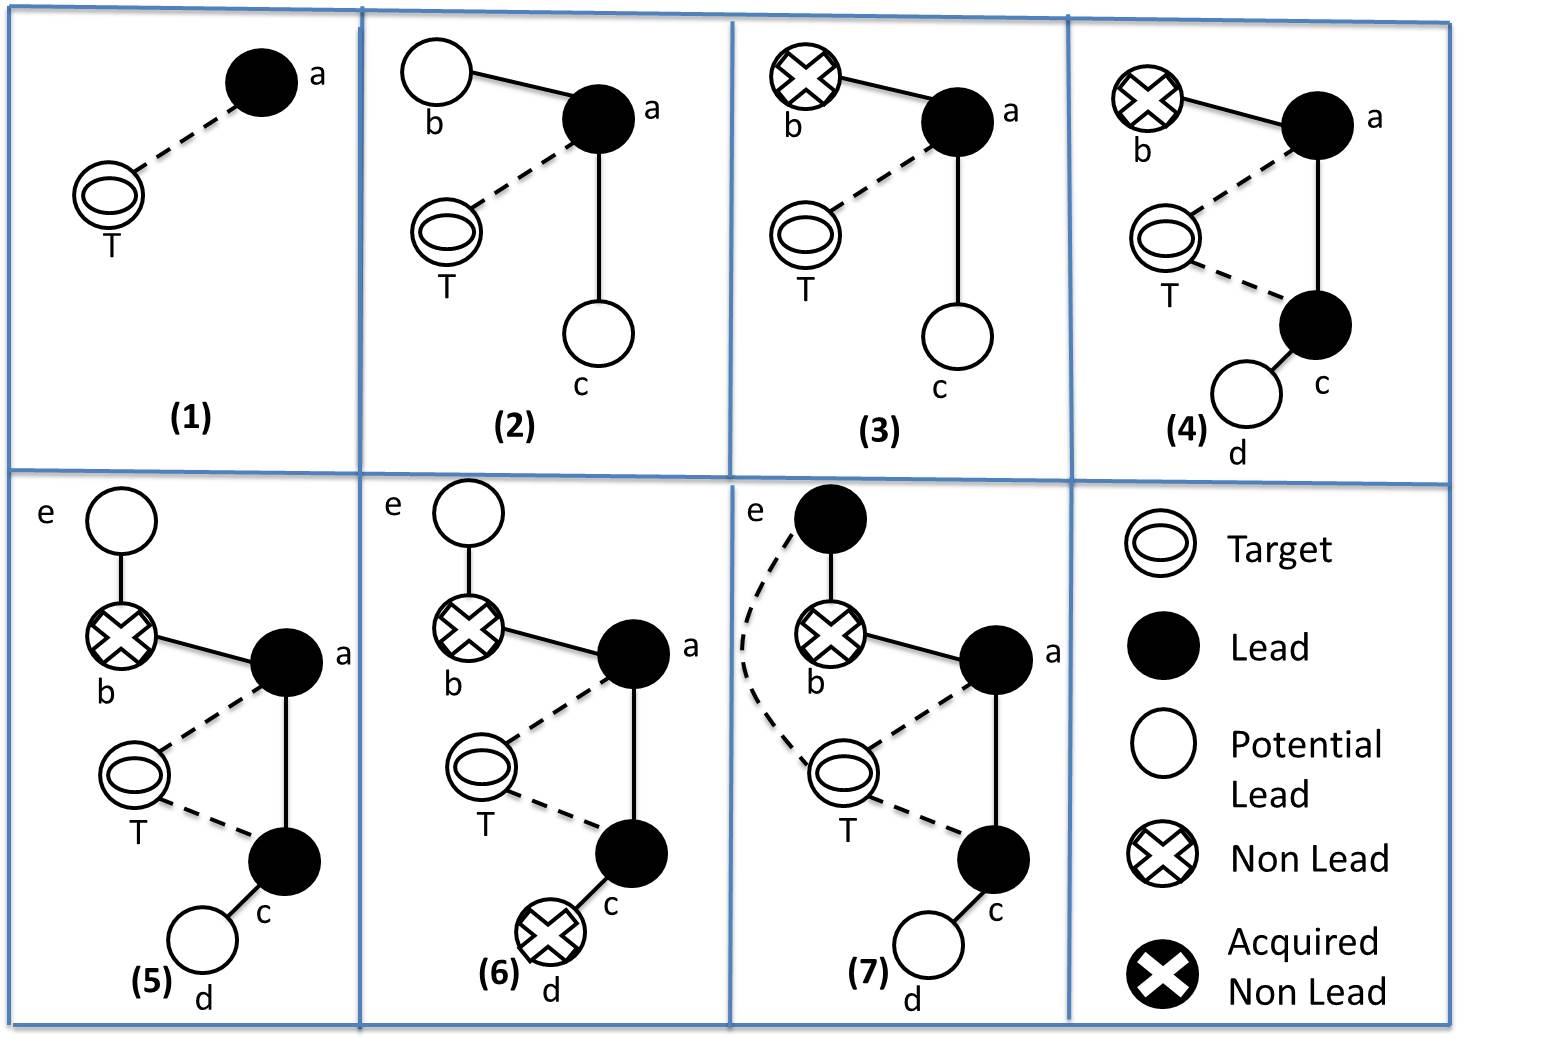
\includegraphics[width=0.75\linewidth]{process-and-legend-new.jpg}
  \caption{An example of a search for leads.}\label{fig:etf_process-and-legend}
\end{figure}
%Figure
%\note{Roni}{Figure fig:etf-process-and-legend does not exist}

Figure~\ref{fig:etf_process-and-legend} shows an execution of ETF. Stages 1-4 are similar to the RTF (see section~\ref{sec:TONICAsHeuristic}). In stage 5 the non lead $c$ is acquired revealing its LOF ($\{e\}$). \islead{$e$} is then performed, revealing that it as a lead. This search process can continue, finding and acquiring more and more leads.
%
%
%A non-lead \(p\) that was discarded in line~\ref{expand:expand-nl-1} since \(d_L(p)>n\) can be reinserted into the OPEN (line~\ref{expand:add-nl-to-open-1}) when a shorter path connecting it to a lead is discovered.
%Non-leads within the tier limit of ETF($n$) are expanded and generate additional potential leads (line~\ref{expand:expand-nl-2}), thus allowing discovery and acquirement of leads that were unreachable in RTF.
%
%As in RTF, the main challenge in ETF(1) is to choose which node to query next in each iteration. Next, we propose several ETF heuristics for this purpose. 
%
%, which action to preform; isLead() operation on a potential lead or a full acquisition of a non lead profile. In this section, as in the RTF section, leads are automatically acquired when discovered.
%
%ETF pseudocode
%The pseudocode of the extended TONIC framework ETF($n$) is also given in Algorithm~\ref{alg:bfs} with several modifications (Lines \ref{expand:add-nl-to-open-1}-\ref{expand:expand-nl-2} preceded with \emph{E}).
%The key difference between RTF and ETF is handling of non-leads which can now be added to OPEN.
%In RTF, a potential lead found to be a non-lead is discarded.
%In ETF($n$), discovered non-leads are reinserted into OPEN (lines~\ref{expand:add-nl-to-open-1}, \ref{expand:add-nl-to-open-2},  and~\ref{expand:add-nl-to-open-3}), to be later considered for expansion if their  $d_L(\cdot)\leq n$ (lines~\ref{expand:expand-nl-1}--\ref{expand:expand-nl-2}).
%Note that the distance of non-leads can change as the search progresses.
%A non-lead \(p\) that was discarded in line~\ref{expand:expand-nl-1} since \(d_L(p)>n\) can be reinserted into the OPEN (line~\ref{expand:add-nl-to-open-1}) when a shorter path connecting it to a lead is discovered.
%Non-leads within the tier limit of ETF($n$) are expanded and generate additional potential leads (line~\ref{expand:expand-nl-2}), thus allowing discovery and acquirement of leads that were unreachable in RTF.
%
%
Since the number of reachable profiles (and reachable non-leads) with ETF is much larger than with RTF, ETF can potentially perform worse than RTF. Thus, the benefit of ETF depends on having an effective heuristic for choosing the best node to expand. In this section we describe several ETF heuristics.

%Problem def


\subsubsection{EFIFO heuristic}
This simple baseline heuristic chooses $\best$ for expansion in a first-in-first-out (FIFO) order. If a potential
lead was chosen as $\best$ and discovered as a non lead, it is removed from the OPEN and reinserted as non lead at the end of OPEN. 
Figure~\ref{fig:etf_process-and-legend} illustrates such an expansion order. Figure~\ref{fig:PROMISE_FIFONL_HYBRID} shows the performance of EFIFO in our data set (described in Section~\ref{sec:btf-experimentalResults}) versus that of BysP, the best RTF heuristic. The $x$-axis is the number of \islead{}
calls. The $y$-axis is the number of leads found by \islead{} up to that point.\footnote{The exact setting of this experiment is provided below in the experimental section.} As can be seen, EFIFO discovers leads slower than BysP but eventually reaches more leads.
%\ref{fig:PROMISE_FIFONL_HYBRID}.


\subsubsection{Hybrid Heuristic}



\begin{figure}[t]

\begin{subfigure}{0.5\columnwidth}%
\centering
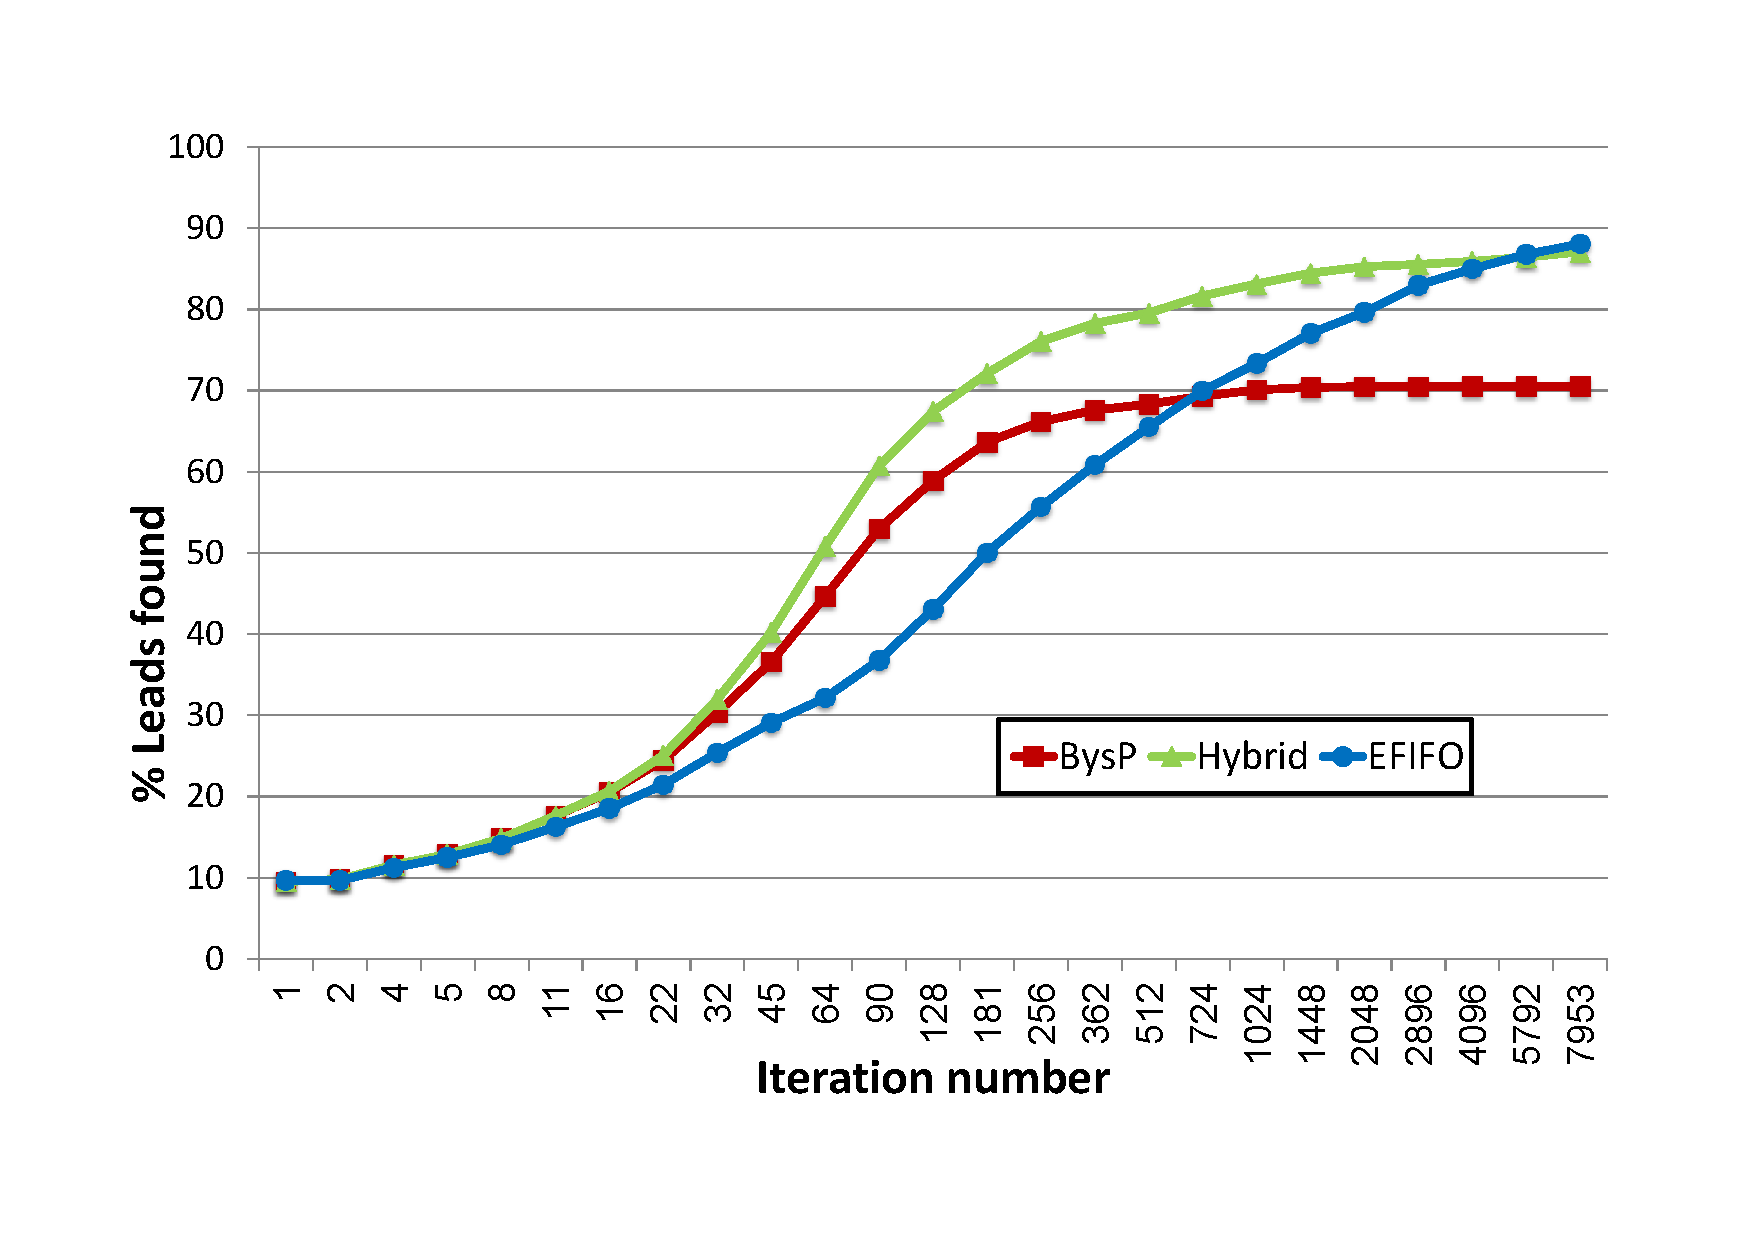
\includegraphics[width=\textwidth, trim={2.0cm 2.5cm 2.5cm 2.0cm},clip]{PROMISE_FIFONL_HYBRID.pdf}
\caption{\label{fig:PROMISE_FIFONL_HYBRID}Hybrid vs. BysP(0) and EFIFO(1)}%
\end{subfigure}
\begin{subfigure}{0.5\columnwidth}
\centering
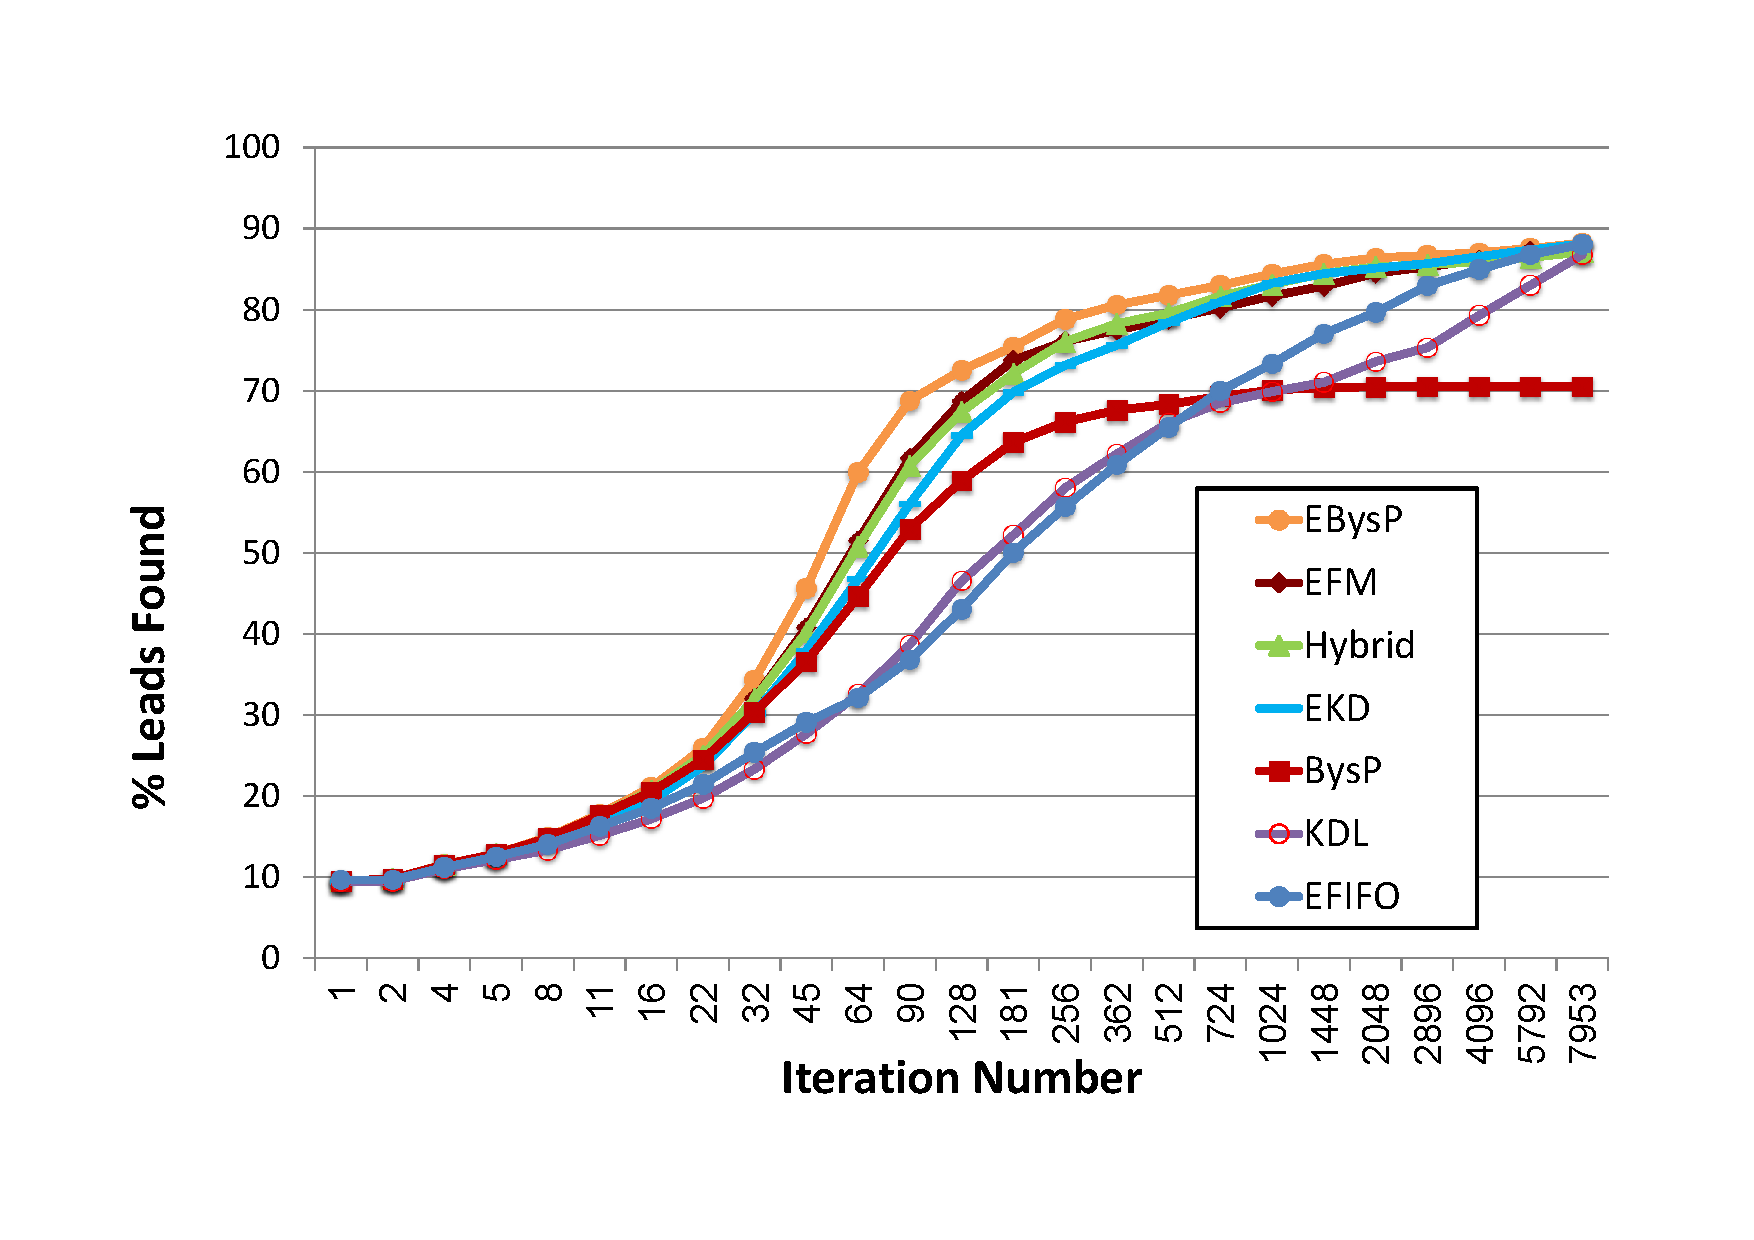
\includegraphics[width=\textwidth, trim={2.0cm 2.5cm 2.5cm 2.0cm},clip]{all_nl_with_promise.pdf}%\vspace{-0.3cm}
\caption{\label{fig:all-nl}All heuristics}%\vspace{-0.3cm}
\end{subfigure}%

\caption{Performance of ETF heuristics. The $x$-axis is number of executed iterations of Algorithm~\ref{alg:bfs}. The $y$-axis is the percentage of leads found by \islead{} up to that point.}
\end{figure}

To enjoy the complementary benefits of BysP, which finds leads fast by effectively focusing on clusters of leads and the extended reachability of EFIFO, we propose an adaptive {\em hybrid} heuristic that starts with BysP and eventually switches to EFIFO. Ideally, we would like to switch as soon as BysP exhausted the set of leads it can reach. To determine the exact switching point we define a bound \(U\) which determines the number of \islead{$\cdot$}~ queries allowed since the last lead was found. If \(U\) unsuccessful \islead{$\cdot$}~queries were done by BysP, the \emph{hybrid} heuristic assumes that BysP has discovered the set of leads it can reach and switches to EFIFO.

We have tried many values for $U$ and have found that the best option is to increment $U$ dynamically according to the following assignment schedule. Initially, set $U$ to some constant. Whenever a lead is acquired (with BysP), $U$ is set to be the number of \islead{$\cdot$}~queries done so far. For example, if a lead was found in the third \islead{$\cdot$} operation then $U$ is set to 3 and if no lead will be found in the next 3 \islead{$\cdot$} operations then we will switch from the BysP heuristic to FIFO. 


Empirical evaluation (see Figure~\ref{fig:PROMISE_FIFONL_HYBRID}) shows that \(hybrid\) is able to outperform both BysP and EFIFO, suggesting that $hybrid$ switches heuristics when EFIFO starts to outperform BysP. 
The $x$-axis in Figure~\ref{fig:PROMISE_FIFONL_HYBRID} corresponds to the number of iterations of the main loop in Algorithm~\ref{alg:bfs} (lines 5--18). 
In each iteration one node is removed from OPEN and is queried according to the Algorithm~\ref{alg:bfs}.

% [R 1.23]
%\subsection{Experimental Results}
%To enjoy the complementary benefits of BysP, which finds leads fasts by effectively focusing on clusters of leads, and the extended reachability of EFIFO, we propose an adaptive {\em hybrid} heuristic that starts the search with BysP and eventually switches to EFIFO. Ideally, we would like to switch as soon as BysP exhausted the set of leads it can reach. To determine the exact switching point we define a bound \(U\) which determines the number of \islead{$\cdot$}~ queries allowed since the last lead was found. If \(U\) unsuccessful \islead{$\cdot$}~queries were done by BysP, the \emph{hybrid} heuristic assumes that BysP has discovered the set of leads it can reach and switches to EFIFO.

%We have tried many values for $U$ and have found that the best option is to increment $U$ dynamically according to the following assignment schedule. $U$ is initially set to some constant. Upon acquisition of a lead (with BysP), \(U\) is set to be the number of \islead{$\cdot$}~queries done so far. For example, if a lead was found in the third \islead()\ operation, U is now set to 3, meaning that unless a lead is found in the next 3 \islead\ operations, the BysP heuristic will be switched to FIFO. 


%Empirical evaluation (see Figure~\ref{fig:PROMISE_FIFONL_HYBRID}) shows that \(hybrid\) is able to outperform both BysP and EFIFO, suggesting that $hybrid$ switches heuristics when EFIFO starts to outperform BysP.  The $x$-axis in Figure~\ref{fig:PROMISE_FIFONL_HYBRID} corresponds to the number of iterations of the main loop in Algorithm~\ref{alg:bfs} (lines 5--18).  In each iteration one node is removed from OPEN and is queried according to the Algorithm~\ref{alg:bfs}.


\subsubsection{Variants of the Known Degree Heuristic}
KD, described above for RTF, expands the potential lead with the highest degree
in the CKG.
Next we discuss how to adapt it to ETF. Let $EKD(p)$ be the degree of $p$ in the
CKG, and let $KDL(p)$  be the number of leads adjacent to $p$ in the CKG.
Since only leads are acquired in RTF, there is at least one lead in every edge
of the CKG. Consequently, in RTF $EKD(p)=KDL(p)=KD(p)$ for every potential lead $p$.
In ETF, $EKD(p)$ and $KDL(p)$ can be different, as a potential lead may be connected to leads and to non-leads. This results in two possible ETF heuristics EKD and KDL, each expanding the node (either potential lead or
non-lead) in $OPEN$ with the highest $EKD(\cdot)$ and $KDL(\cdot)$, respectively.



\begin{figure}
\centering
\begin{subfigure}{.4\textwidth}
\centering
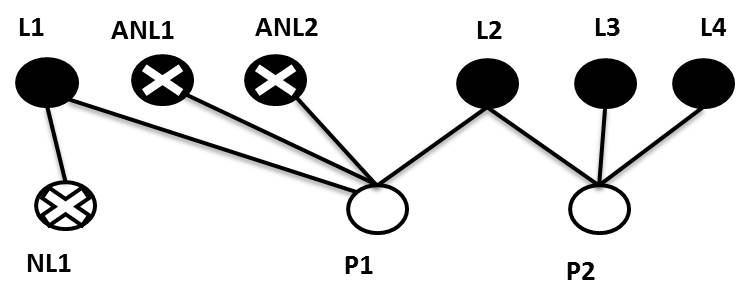
\includegraphics[width=\linewidth]{NL_BASE.jpg}%\vspace{-0.3cm}
%\vspace{0.4cm}
\caption{EKD and KDL}\label{fig:NL_Heuristics}%\vspace{-0.3cm}
\end{subfigure}%
\begin{subfigure}{.35\textwidth}
  \centering
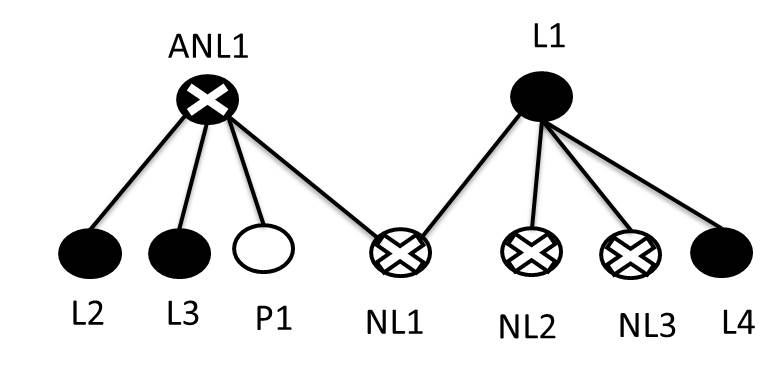
\includegraphics[width=\linewidth]{PROMISENL.jpg}%\vspace{-0.3cm}
%\vspace{0.4cm}
  \caption{EBysP}
  \label{fig:PROMISENL}
\end{subfigure}%
\begin{subfigure}{.25\textwidth}
  \centering
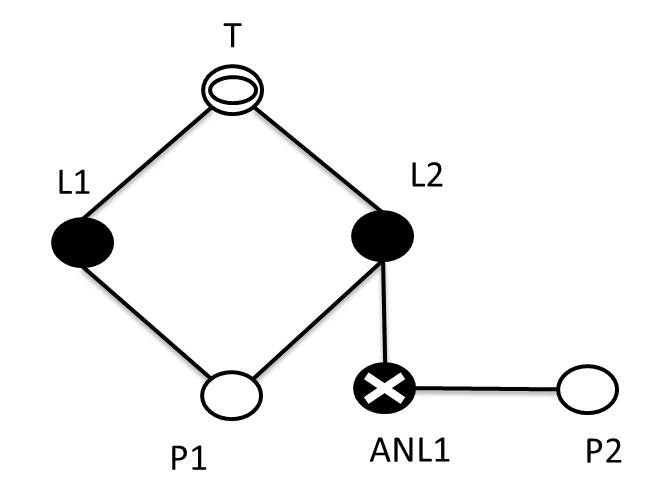
\includegraphics[width=\linewidth]{fm.jpg}
  \caption{EFM}
  \label{fig:efm}
\end{subfigure}%

\caption{Examples of the ETF heurisitics.}
\label{fig:efm-and-ebysp}

\end{figure}


Figure~\ref{fig:NL_Heuristics} depicts a CKG that demonstrates the difference between EKD and KDL. The legend for this figure is the same legend shown in Figure~\ref{fig:bfs_example}. There are three profiles that can be
expanded: NL1, P1 and P2. KD will expand P1 since $EKD(P1)=4$, $EKD(NL1)=1$, and
$EKD(P2)=3$, while KDL will expand P2 since $KDL(P2)=3$, $KDL(P1)=2$, and
$KDL(NL1)=1$.


The intuition behind EKD and KDL differ. EKD is based on the assumption that
leads tend to cluster together, and thus a profile with many adjacent leads
suggests that this profile is itself lead or is adjacent to many other leads.
KDL is based on the assumption that a profile with a high degree in the CKG has
a high degree in the underlying graph (the OSN), and thus expanding it would
result in finding many other profiles, some of which would be leads.
Our experiments showed that EKD performs significantly better than
KDL in ETF(1) (as shown in Figure \ref{fig:all-nl} explained in the
experimental section).

\subsubsection{BysP and FM Heuristics for ETF}



BysP and FM were the best performing RTF heuristics (see Section~\ref{sec:btf-experimentalResults}), and they can be easily adapted for ETF. The key difference between RTF and ETF is that non-leads can be acquired, and thus while in RTF neighbors of profiles that are considered for expansion (either \islead{} or \acquire{}) were leads, in ETF the neighborhood of a profile that was not acquired yet may also contain non-leads. This requires slight modifications to the BysP and FM heuristic computation. 

For BysP, the BysP score ($BysP(p)$) of a profile $p$ in ETF would aggregate the promising factor of all its neighbors, regardless if they are leads or not. For FM, the Friends Measure would count links between all neighbors of $p$, non-leads included, and all the known leads. To distinguish between BysP and FM for RTF and for ETF, we denote the latter EBysP and EFM, respectively.

Note that both EBysP and EFM expand the profile with the highest score in $OPEN$ (each according to its scoring function), regardless if it is a potential lead or a non-lead. If that profile is a potential lead, then an \islead{} query is applied to it and it is acquired if it is found to be a lead. If the best profile is a non-lead, then it is acquired. 

%BysP was the best performing heuristic for RTF~\cite{stern2013target}. BysP chooses to expand the potential lead $pl\in OPEN$ having the highest
%$BysP(pl)=1-\prod_{m\in L(pl)}(1-pf(m))$. A small modification is required in order to apply it to ETF as follows:
%\[ EBysP(p)=1-\prod_{m\in L(p)\cup NL(p)}(1-pf(m)) \]
%\vspace{0.1cm}\\
%$~~~~~~~~~~~EBysP(p)=1-\prod_{m\in L(p)\cup NL(p)}(1-pf(m))$\\
%\vspace{0.1cm}

%The key difference between $BysP(p)$ and $EBysP(p)$ is that $BysP(p)$ only aggregates the $pf(\cdot)$ values of the leads that are adjacent to $p$ ($L(p)$) 
%while $EBysP(p)$ aggregates over all the acquired neighbors of $p$ ($L(p)\cup NL(p)$). 
%We use EBysP to denote the ETF heuristic that expand the profile $p$ with the highest $EBysP(\cdot)$ in $OPEN$, regardless if $p$ is a potential lead or a non lead.


To illustrate  EBysP, consider Figure~\ref{fig:PROMISENL}. $OPEN$ contains P1,
NL1, NL2, and NL3. These profiles are connected to two acquired profiles, ANL1
and L1, having $pf(\cdot)$ values of $\frac{2}{3}$ and $\frac{1}{4}$, respectively. As a result, P1, NL1, NL2, and NL have $EBysP$ values of
$\frac{2}{3}$, $\frac{9}{12}$, $\frac{1}{4}$, and $\frac{1}{4}$, respectively, and therefore EBysP expands NL1.







%Liron: to delete the FM example?
Figure~\ref{fig:efm} demonstrates EFM. There are two potential leads P1 and P2. According to the EFM definition presented, $fm(T,P1)=2$ and  $fm(T,P2)=1$ (ANL1 is in P2's neighborhood and it is friends with L2 which is in the target's neighborhood). Thus, P1 will be acquired prior to P2.

%\note{Roni}{Need to consider removing both examples. Or, even better, have these examples where we have BysP and EBysP to show the difference, and the same for FM and EFM. Thoughts?}

%\subsubsection{EFM}
%The FM heuristic, described above for RTF, expands the potential lead with the highest Friend Measure score. In RTF, the potential leads' neighborhood contained only leads since they were the only profiles acquired. In ETF however, non leads can also be acquired and therefore the FM heuristic should be adjusted to count both types of profiles and the link between them as mutual friends. To distinguish between FM for RTF and this adjusted FM for ETF, we denote the latter as ETF. 
% We tried FM
%Formally, the extended friends measure ($efm$) between a profile \(p\) ans the target is: 
%\[
%efm(t,p)= \sum\limits_{x\in L}~~\sum\limits_{y | (p,y)\in E} \delta(x,y)
%\]
%\noindent where \(E\) is the edges in the CKG, \(L\) is the set of leads and $\delta(x,y)$ is defined as:
%\begin{equation}
%\delta(x,y) = \begin{cases}
%1 &\text{if $x=y$ or $(x,y)\in E$ or $(y,x) \in E$}\\
%0 &\text{Otherwise}
%\end{cases}
%\end{equation}


%X represent the target's neighborhood, which contains only leads (every profile connected to the target is considered a lead) and y represent $p$'s neighborhood.
%The EFM formula is similar to the FM formula. However now y can represent both leads and non leads profiles connected to a profile $p$. In addition, the profile $p$ considered for expansion can now be either a potential lead or a non lead. \note{Roni}{The reviewers are not that dumb, and repeating to much will insult them (happend to me)}

%The ETF heuristic chooses as $best$ the candidate $p$ with the highest $efm(target,p)$. Experimentally, we show later (see Figure \ref{fig:all-nl}) that $efm$ performs reasonably well as a TONIC heuristic.



In order to evaluated the performance of ETF(1) with the proposed heuristics we used the same benchmark set of targets and initial leads as was used in the RTF experiments earlier (Section~\ref{sec:btf-experimentalResults}). However now, the relevant neighborhood of each target is larger since it contains an additional tier. 
%Figure \ref{fig:googleNewTarget} represents the relevant neighborhood in ETF for the same target that was presented in Figure~\ref{fig:net}.  
%\note{Roni}{Liron. What would be really cool is to show for the same profile how its relevant neighborhood looks in tier 0 and tier 1. Can you do this easily?}

%\begin{figure}[!hb]
%\centering
%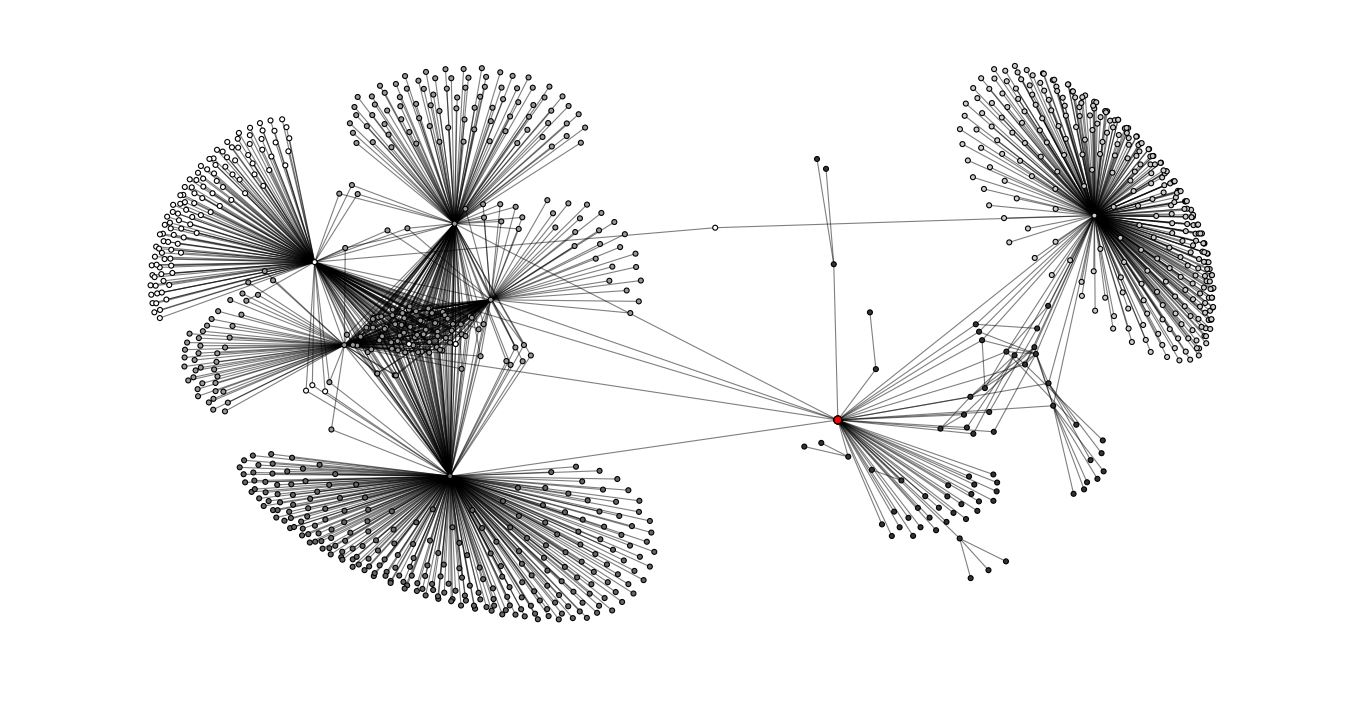
\includegraphics[width=0.7\linewidth]{google_new_ETF.JPG}%\vspace{-0.3cm}
%\caption{Sample network of the ETF relevant neighborhood of a target}\label{fig:googleNewTarget}%\vspace{-0.3cm}
%\end{figure}


Figure~\ref{fig:all-nl} compares the percentage of leads found (the $y$-axis) out of all the possible leads by each of the proposed ETF heuristics as a function of the iteration percentage (the $x$-axis).
%The iteration in the ETF, as oppose to the RTF, does not represent only \islead{} operations but also non leads acquisitions. \note{Roni}{First, the reader at this stage will be tired of hearing about this. Second, there's the issue of not counting the acquired leads, which I'm not sure we want to raise.}
%In each iteration the search preforms one of the two mentioned actions.
 For reference, we also present the results for BysP (which was the best RTF heuristic).
At the very beginning of the search, all heuristics perform similarly because the CKG
is too small to be informative and the search is almost blind. As the search
progresses and the CKG grows, EBysP quickly gets better than other  heuristics,
finding more leads faster. In particular, EBysP substantially outperforms BysP throughout the search. 
For example, after  0.8\% of the iterations, BysP found slightly more than 40\% of the leads, while EBysP
found approximately 60\%. This result demonstrates that intelligent acquisition
of non-leads not only enables reaching more leads eventually (as shown in
Table~\ref{tab:BTFtiers}), but also significantly speeds up the acquisition of
leads during  early stages of the search.
%\note{Roni}{A more sensible x-axis for this figure would be nice. It is not clear if it is logarithmic, of some predefined steps with no logic behind it.}


All studied heuristics are computationally efficient as they analyze the
neighborhood of the evaluated profile $p$ only up to two hops away. KD is the
simplest heuristic that only considers the connectivity of $p$. Surprisingly,
its performance is not a lot worse than the performance of the more sophisticated
heuristics EBysP and FM and much better than the performance of KDL which is
more focused toward leads.




\section{Cost-Benefit Analysis}
\label{sec:costbenefit}

Up until now, we focused on the budged objective (represented by the $x$-axis). The experiments showed given $B$ operations, how many leads have we found?
%, denoted as Utility.
In this section we analyze the proposed TONIC frameworks and heuristics from the perspective of the second objective function we proposed, which aims at maximizing the net gain (Definition~\ref{def:gain}). 
The net gain is roughly related to the steepness of the slopes in Figure~\ref{fig:all-nl}. A steep slope corresponds to finding many leads with few queries, which means high net gain, while a flat line means costs of queries are spent but no leads are found, which means decreased net gain. A trend that is very clear in Figure~\ref{fig:all-nl} is that during late stages of the search the frequency of leads decreases and the slopes become flatter. Therefore, the net gain may drop to a point where the search process is not worthwhile.


\begin{figure}

\centering
\begin{subfigure}{.55\textwidth}
  \centering
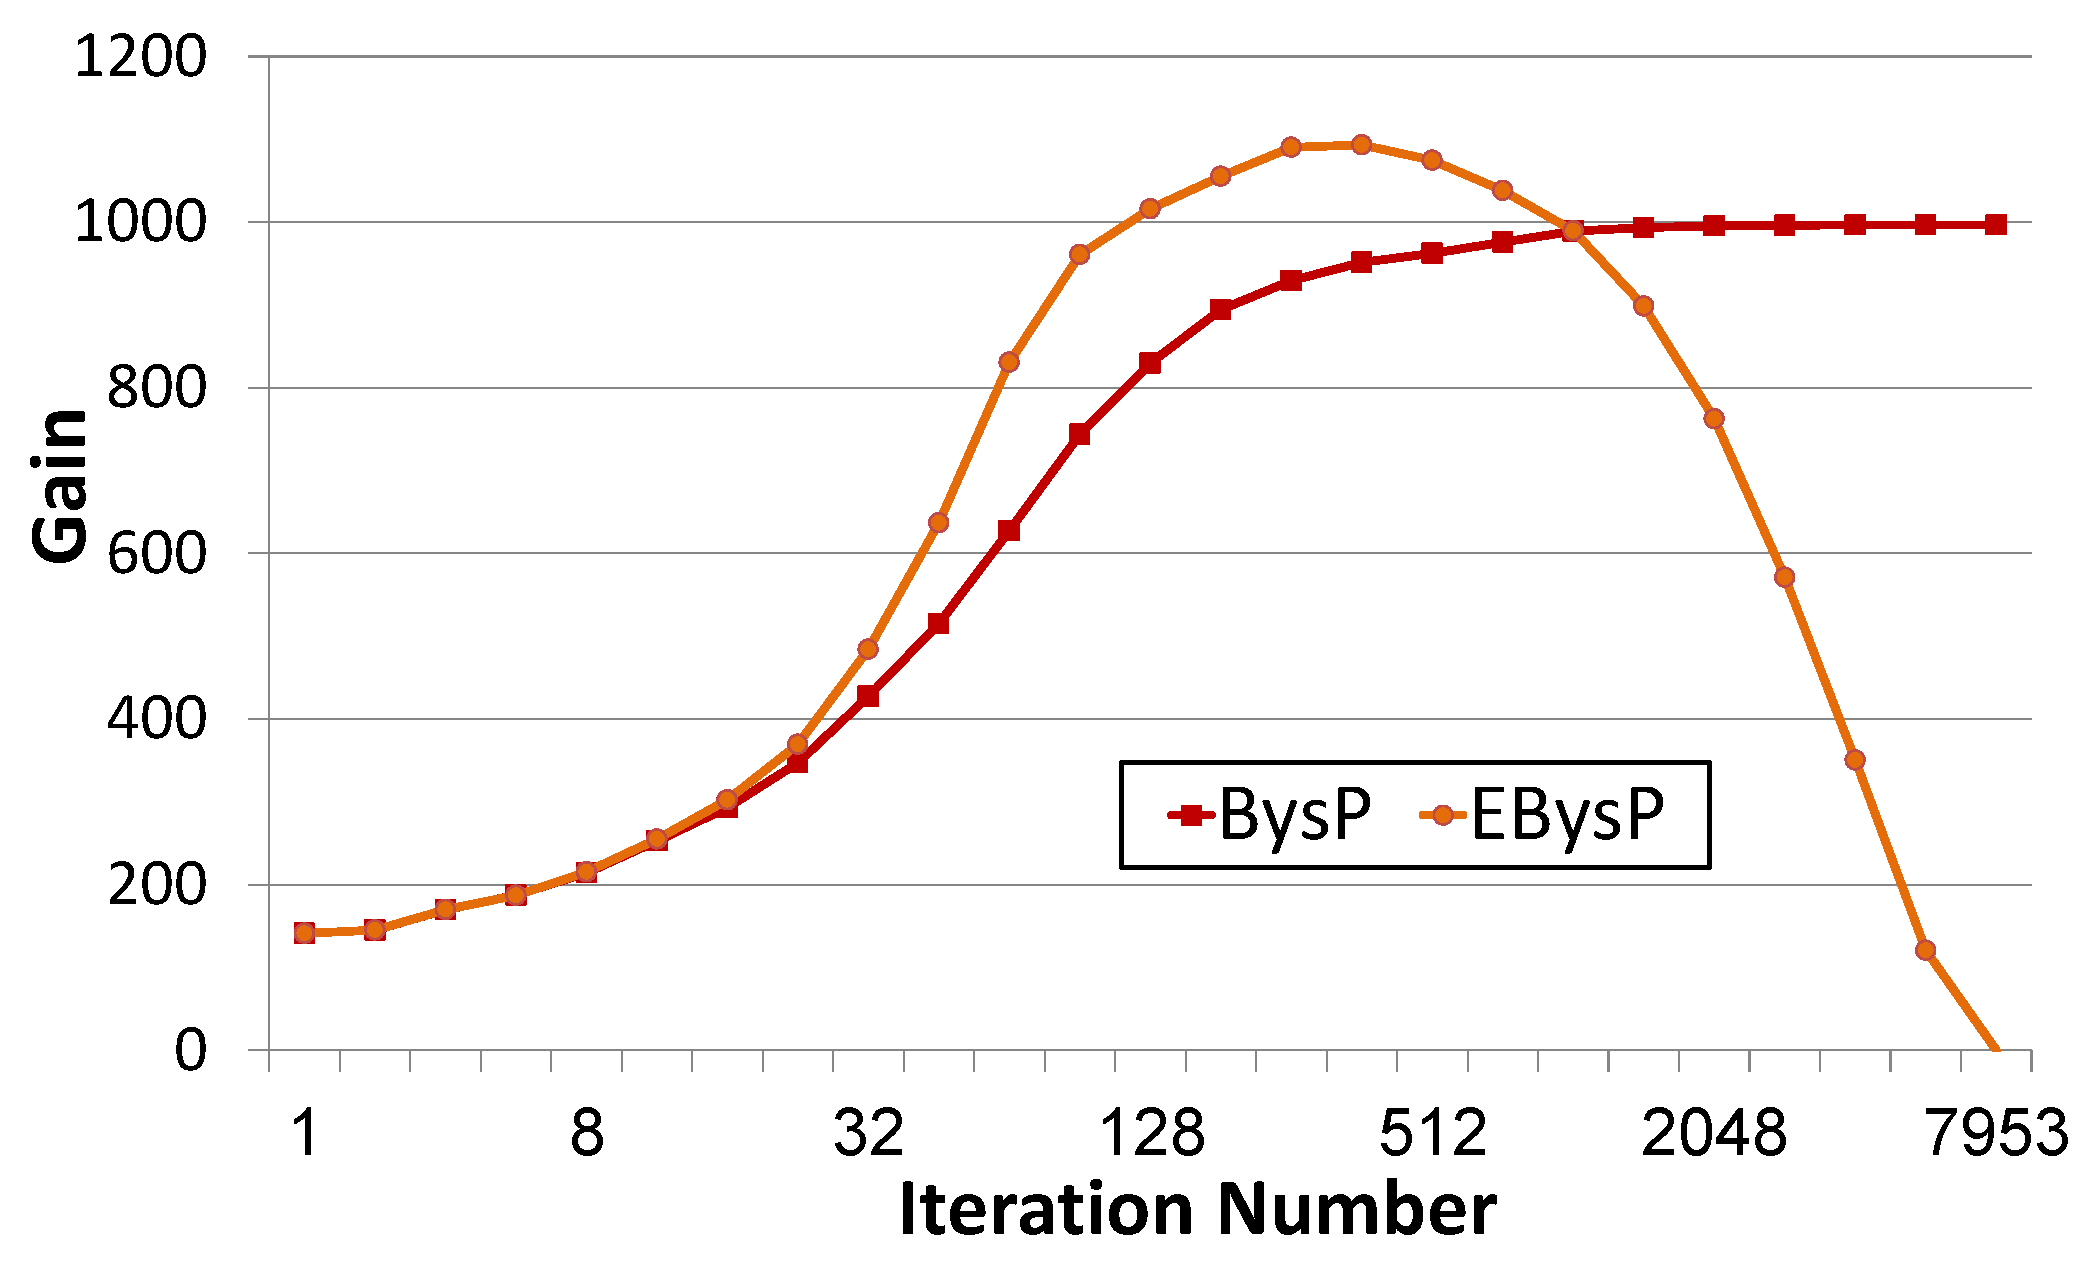
\includegraphics[width=\linewidth]{Cost_Iteration.pdf}%\vspace{-0.3cm}

\caption{Net gain for $R_{Acquire}$=40 and $C_{Acquire}$=1}%\vspace{-0.3cm}
\label{fig:CostIteration}
\end{subfigure}%
\quad
\begin{subfigure}{.3\textwidth}
  \centering
\begin{tabular}{c|r|r}
Reward & BysP & EBysP \\\hline
100 & 2529.45 & {\bf 3100.89} \\
%50 & 1251.95 & {\bf 1495.29} \\
10 & 229.95 & {\bf 250.55} \\
5 & 102.20 & {\bf 104.96} \\
4 & 76.65 & {\bf 76.71} \\
3 & \textbf{51.10} & 49.17 \\
2 & \textbf{25.55} & 22.50 \\
%1.5 & \textbf{12.775} & 10.11 \\
1 & 0 & 0 \\
%0.5 & -1.81 & -1.81 \\
%0.1 & -3.258 & -3.258 \\
\end{tabular}%\vspace{-0.3cm}
\caption{Maximal gain for different $R_{Acquire}$ values}%\vspace{-0.3cm}
\label{tab:Reward}%\vspace{-0.2cm}
\end{subfigure}

\caption{Analysis of net-gain of the best ETF and RTF heuristics.}
\label{fig:net-gain}
\end{figure}


Figure~\ref{fig:CostIteration} demonstrates this, showing the net gain ($y$-axis) as the search progresses ($x$-axis, number of \acquire{} queries executed) for BysP and EBysP. In this experiment we set the cost of \islead{} to be zero, the cost of \acquire{} to one, and the reward of finding a lead is 40.

We chose to evaluate only the BysP and EBysP heuristics because BysP is the best heuristic for RTF(=ETF(0)) and EBysP is the best heuristic for ETF(1). First, observe that the gain of BysP does not decrease throughout the search. This is because RTF only acquires leads, and thus whenever a cost is spent on \acquire{} it is immediately followed by a reward (of passing this profile to the information extraction phase). Thus, the gain in RTF cannot decrease unless either $C_{Acquire} > R_{Acquire}$ or $C_{IsLead}$ is not negligible.



ETF(1) allows acquiring non-leads. When a non lead is acquired, its acquisition
is not followed by immediate reward. However, the acquisition of non leads can
be viewed as a long-term investment, leading to higher rewards and gain in the
future. Indeed, as shown in Figure~\ref{fig:CostIteration} the acquisition of
non leads by EBysP results in much more frequent discovery of leads at the
first stages of the search and overall higher gain compared to BysP.
However, when leads are exhausted, EBysP looses the previously accumulated
reward on useless exploration of the network and may eventually reach negative
gain. In order to gain the most from EBysP one needs to determine when the
search process should be halted. While we leave development of sophisticated
stop conditions for future work, we illustrate next the potential gain of having
such a mechanism.

  


Table~\ref{tab:Reward} shows the maximal gain achievable for BysP and EBysP, for different values of $R_{Acquire}$ and assuming that $C_{Acquire}$=1 and $C_{IsLead}$=0. 
BysP reaches a maximal gain higher than EBysP when \(R_{Acquire} \leq 3 \), and this reverses when $R_{Acquire}\geq 4$. This is reasonable because larger $R_{Acquire}$ makes the long term investment of EBysP in
acquiring of non leads worthwhile.


\begin{figure}
\centering
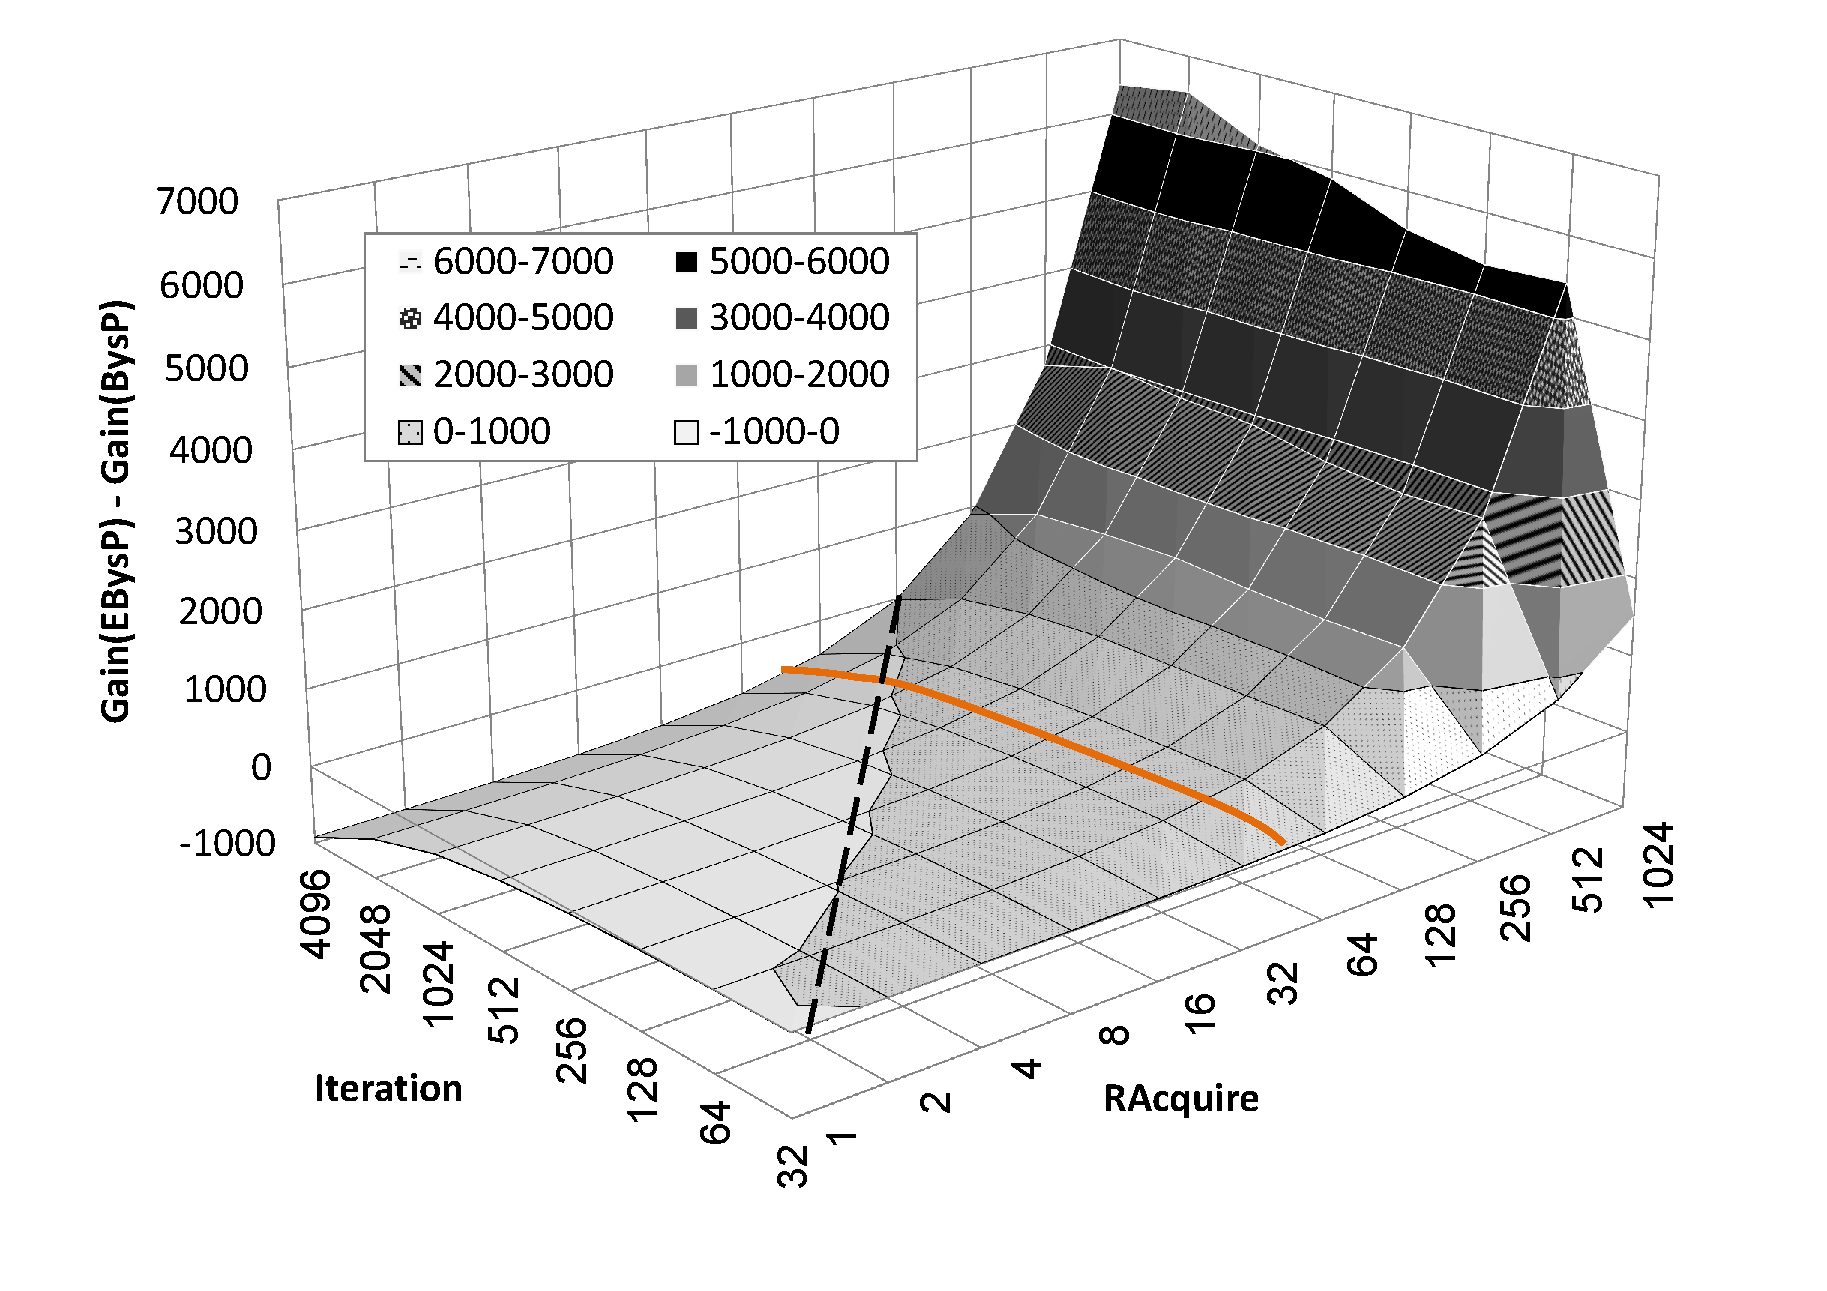
\includegraphics[width=0.7\linewidth]{reward.pdf}%\vspace{-0.3cm}
\caption{The difference in net gain between BysP(0) and BysP(1)}%\vspace{-0.3cm}
\label{fig:reward3d}
\end{figure}



To gain a deeper understanding of the gains of BysP and EBysP throughout the
search, Figure~\ref{fig:reward3d} shows the difference between their gains (vertical-axis $\uparrow$) as a function of \(R_{Acquire}\)
(horizontal-axis $\nearrow$) and the number of iterations (depth-axis
$\nwarrow$). For example, the solid line at \(R_{Acquire}=40\) represents the
difference between gains of EBysP and BysP as depicted in
Figure~\ref{fig:CostIteration}. The dashed line represents the relation between
\(R_{Acquire}\) and iterations where the gains of both heuristics are equal. EBysP (using ETF(1))
benefits from higher rewards and suffers for longer executions, while BysP (using RTF) is a valid choice if $R_{Acquire}$ is not much larger than $C_{Acquire}$ and we expect a long execution. 
Thus, the choice of between BysP and EBysP could be determined upfront if one knows the
number of iterations the search will be run, $R_{Acquire}$, and $C_{Acquire}$. 


\section{TONIC as an Information Retrieval Task}
\label{sec:ir}
%Considering TONIC as an Information Retrieval task allows using known IR metrics for comparing the overall performance of TONIC heuristics. In particular, we consider two such metrics: the area under the ROC curve (AUC) and the discounted cumulative gain (DCG)~\cite{dcg}. 


TONIC can be viewed as an Information Retrieval (IR) task, where the task is to retrieve as many leads as possible. % retrieves an ordered list of profiles given a {\em query} in form of the target and the set of initial leads. IR responses are evaluated based on the positions of relevant and irrelevant results within the ordered list, that is leads and non-leads respectively in case of TONIC.  
Assuming the solver is stopped after performing $x$ \islead{} queries, the {\em true positive rate} (TPR) is the fraction of leads out of the \(x\) profiles and the {\em false positive rate} (FPR) is the fraction of non-leads, respectively. 
The well-known {\em receiver operating characteristic} (ROC) curve~\cite{croft2010search} measures the true positive rate (TPR) as a function of the false positive rate (FPR) for various values of \(x\). A larger area under the ROC curve (AUC) indicates a better solver. 

Figure~\ref{fig:auc} shows the average AUC of the algorithms: FIFO, EFIFO, FM , EFM, BysP and EBysP. The RTF heuristics (run under RTF)  are colored in blue and the ETF heuristics (run under ETF(1)) are colored in purple. AUC results show trends similar to Figure~\ref{fig:all-nl} and Figure~\ref{fig:checkedVsFound}, as could be expected. However it is interesting to see that despite the fact that EFIFO eventually finds more leads then BysP, it's average AUC is still lower, since it preforms worse during most of the search.



%In TONIC, most potential leads are not leads, and thus in general the number of non-leads found is very similar to the total number of \islead{} preformed. Thus, the ROC curve for TONIC greatly resembles the cost-benefit curve shown in Figure~\ref{fig:checkedVsFound} and Figure~\ref{fig:all-nl} (this was also observed empirically).






\begin{figure}
\centering
\begin{subfigure}{.5\textwidth}
  \centering
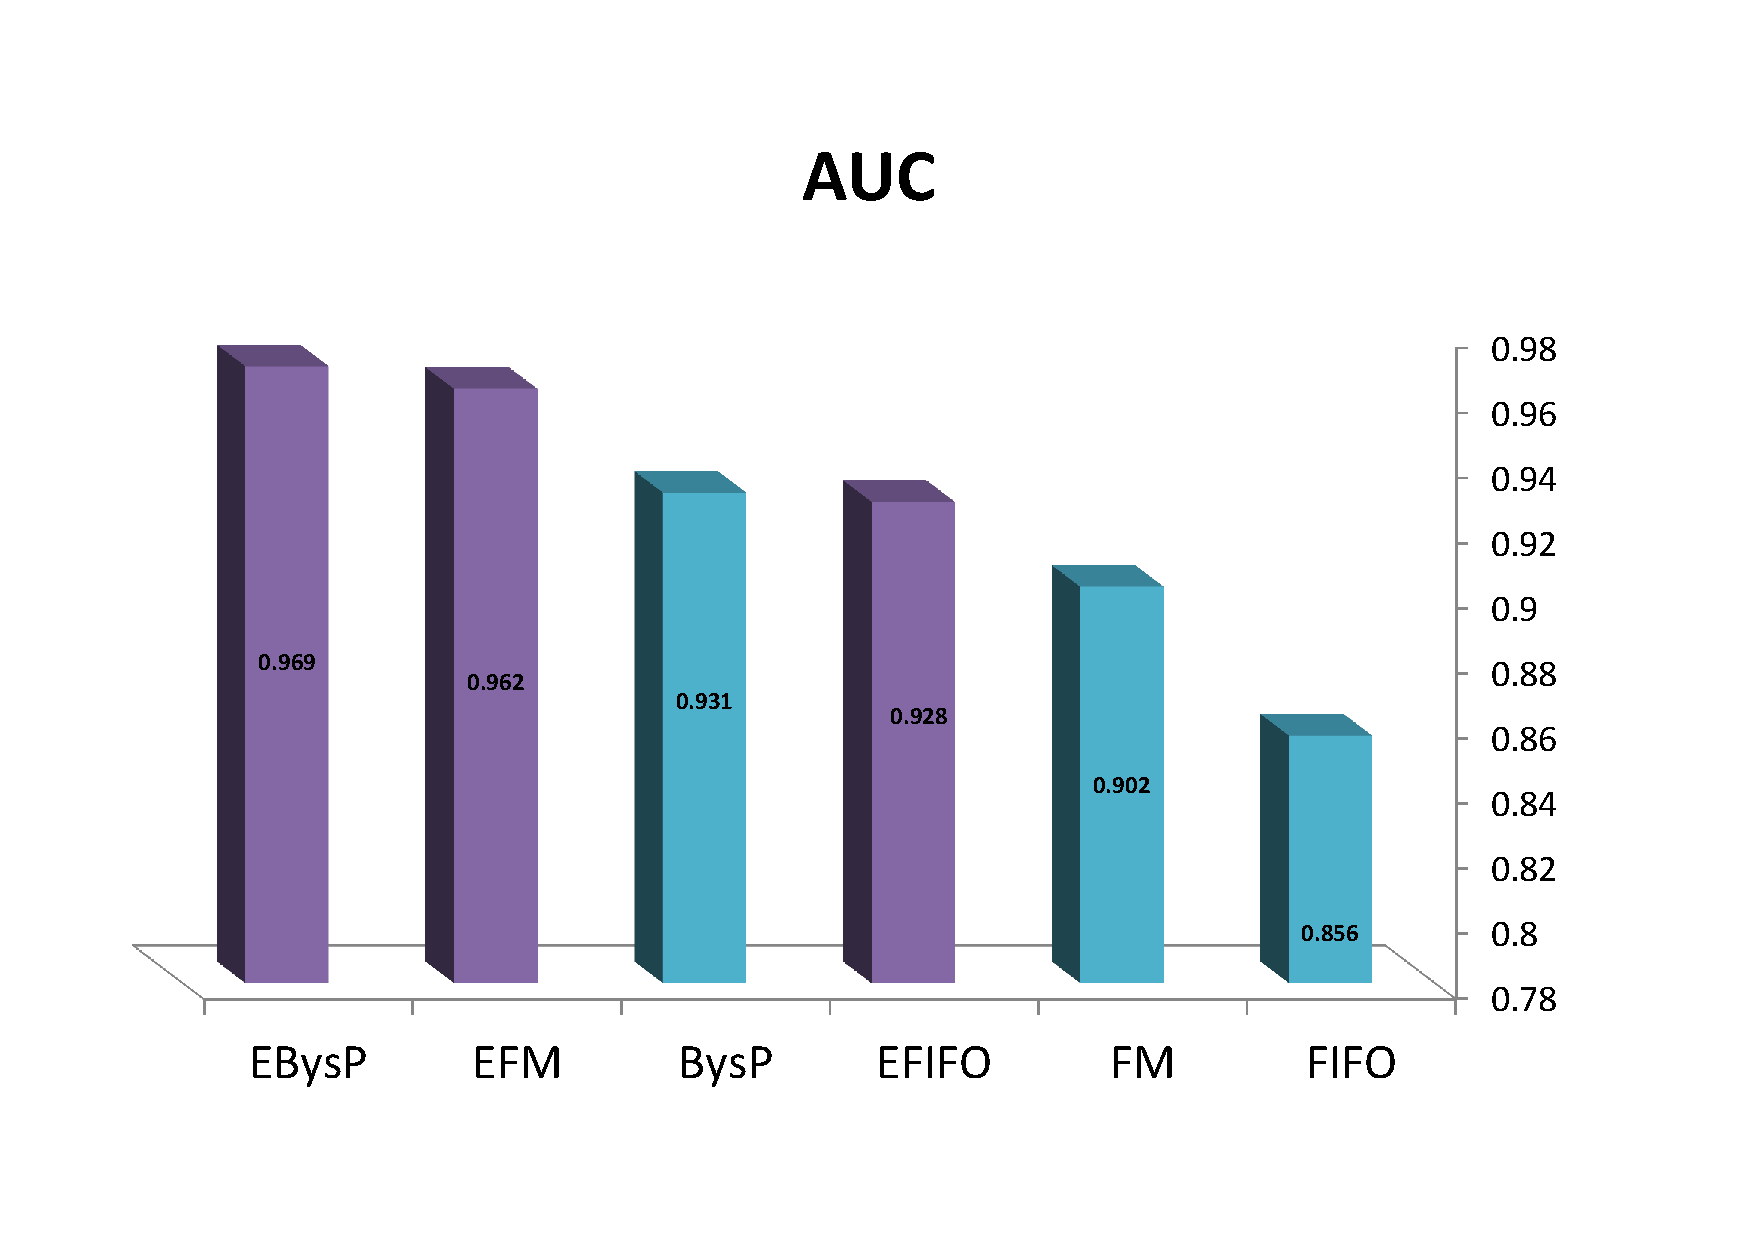
\includegraphics[width=\linewidth,  trim={2.0cm 2.5cm 2.5cm 5.5cm},clip]{AUC_ALL.pdf}
\caption{Average AUC}
\label{fig:auc}
\end{subfigure}%
\begin{subfigure}{.5\textwidth}
  \centering
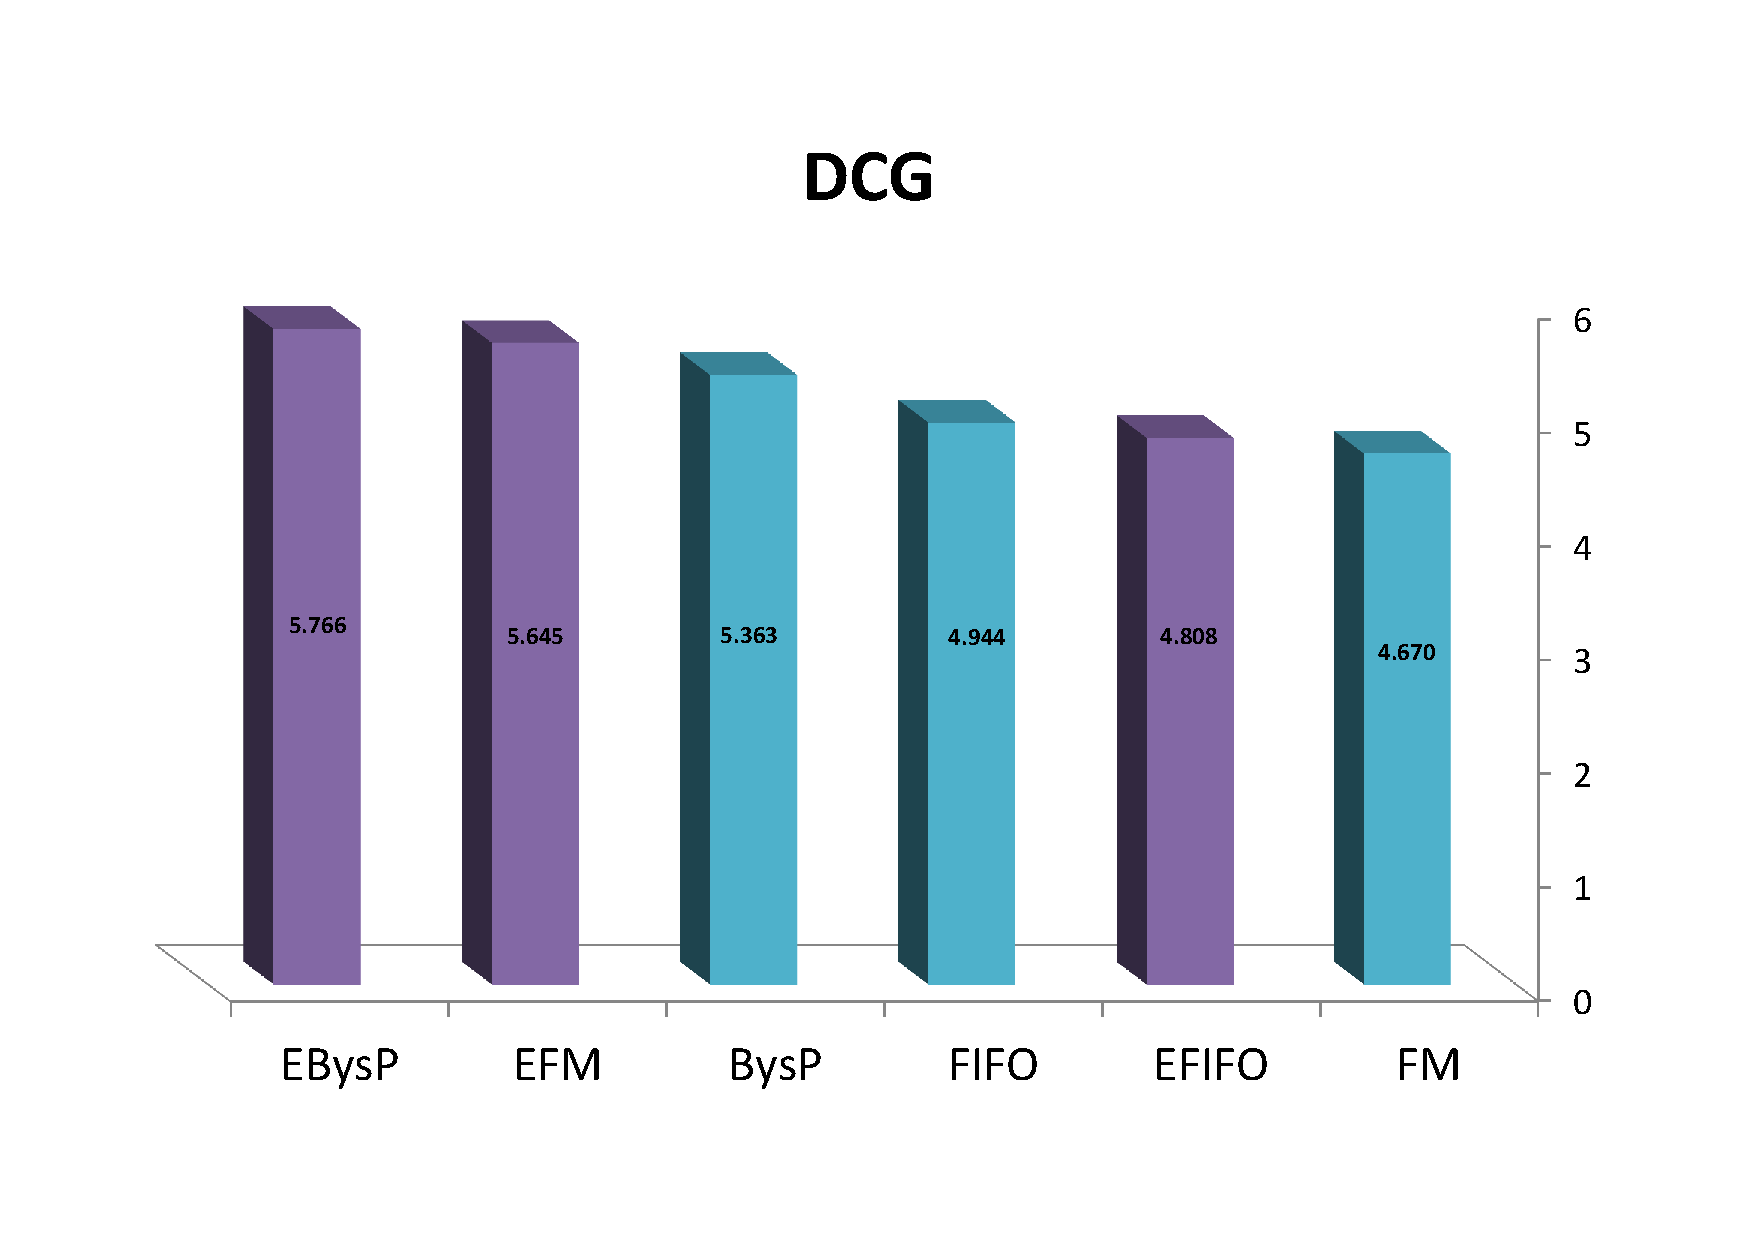
\includegraphics[width=\linewidth,  trim={2.0cm 2.5cm 2.5cm 5.5cm},clip]{DCG_AllAlgo.pdf}
\caption{Average DCG}
\label{fig:dcg}
\end{subfigure}
\caption{Evaluating TONIC heuristics using IR measures.}
\label{fig:auc-and-dcg}
\end{figure}




 

Discounted cumulative gain (DCG)~\cite{dcg} is yet another metric for evaluating the quality of an ordered  sequence of results.
DCG accumulates the gain of finding the relevant results, i.e. the leads, such that the closer the lead is to the beginning of the sequence the higher its gain. 
Every \islead{} query increases the network footprint of the intelligence collection process and with the footprint grows the chance the the process will be discovered or the OSN service will block future acquisitions. 
Therefore, every \islead{} query reduces the gain from further lead acquisitions and it is important to spot the leads as early in the search process as possible.
Let \(p_1,p_2,\ldots\) be the profiles sorted by the order in which \islead{} query was applied to them. 
DCG is computed by $DCG=IsLead(p_1)+\sum_{i=2}^n \frac{IsLead(p_i)}{log_2 i}$, where \islead{\(p_i\)}\(=1\) if the $i^{th}$ profile is a lead and \islead{\(p_i\)}\(=0\) otherwise. 

%[R 3.2]
Figure~\ref{fig:dcg} shows the average DCG of the algorithms mentioned before. First, observe that in terms of DCG, using EFIFO yields worse results than using FIFO. This is in contrast to the AUC results (Figure~\ref{fig:auc}), where EFIFO yielded higher AUC compared to FIFO. 
This advantage of FIFO in terms of DCG is due to the fact that leads more densly populate the first tier. Therefore FIFO will find more leads in earlier iterations -- yielding higher DCG -- since it only searches the first tier and thus its search is less scattered. Thus, in general, for a given TONIC heuristic it may be better to use RTF than ETF if one wants to maximize DCG. 
%[R 3.2]
However, when the more intelligent TONIC heuristics are used, we observe again the benefit of using ETF. This is somewhat surprising, as one could expect that the first leads being found are from the first tier and thus RTF may perform better than ETF. These results suggest that the best performing TONIC heuristics -- BysP and FM -- are intelligent enough to consider expanding non-leads only when it is helpful, thus resulting in finding more leads than in RTF even in early iteration of the search. 
In summary, we observe that EBysP and EFM are robust across both AUC and DCG, showing the best performance in both measures. 

%Note that EBysP is in general robust across both AUC and DCG and that both FM and BysP had shown improvement both in AUC and in DCG when implemented in ETF (EFM, EbysP).



% \subsection{Effects of Network Topology Characteristics}
% Next we investigate the network topology characteristics that influence the performance of the proposed TONIC heuristics.
% For that purpose, we will examine the performance of both RTF and ETF heuristics on the DBLP network \cite{yang2012defining} as an additional OSN to the Google+ network previously discussed.

% \begin{figure}
% \centering
% 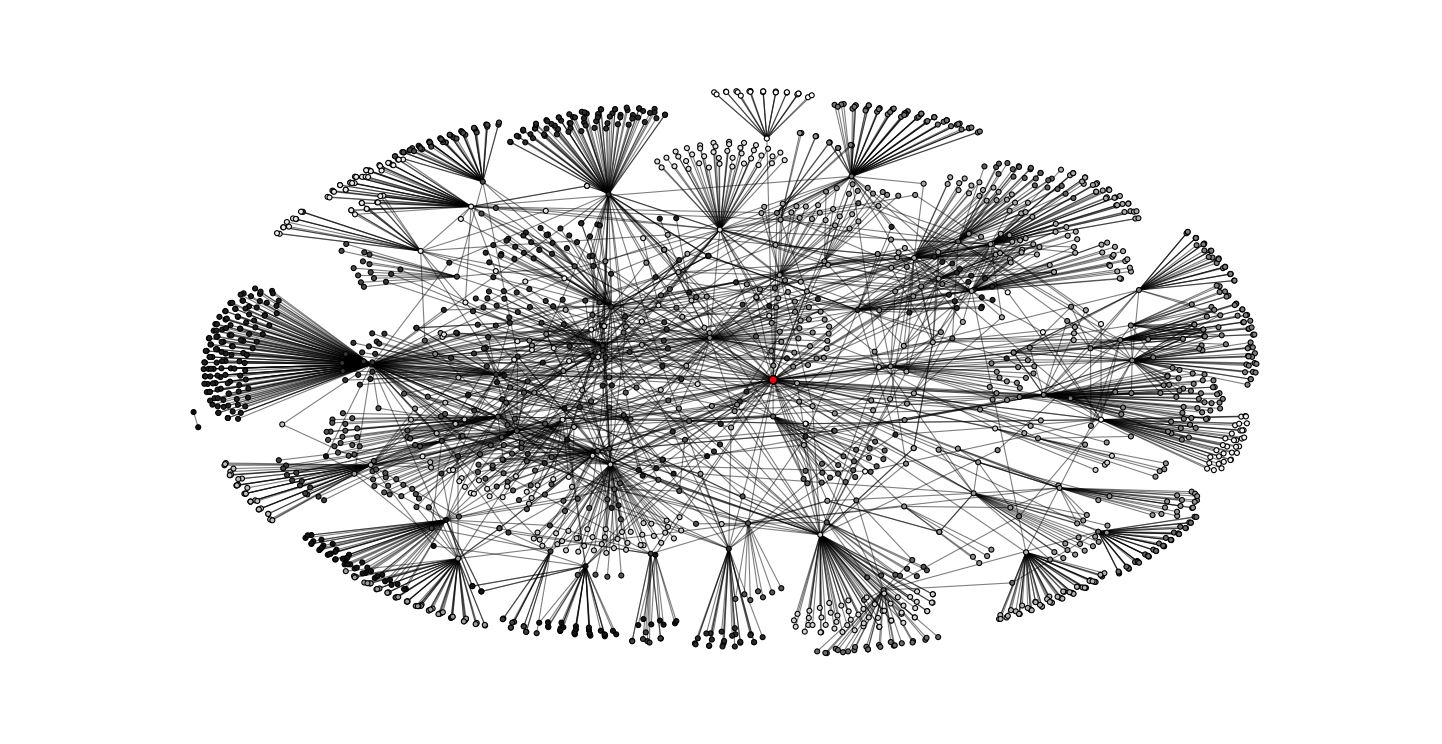
\includegraphics[width=\linewidth]{dblp_target1.JPG}%\vspace{-0.3cm}
% \caption{\label{fig:dblpTarget}Sample network of the relevant neighborhood of a target in DBLP network
% number}%\vspace{-0.3cm}
% \end{figure}


% We have taken 100 different targets with more than 30 friends and set 3 random friends as initial leads (same as we did for the Google+ network). An example of tier(1) of one of the targets in DBLP is presented in Figure~\ref{fig:dblpTarget}.
% The search was preformed on four heuristics; The RTF and ETF baselines (FIFO and EFIFO) and the dominating heuristics (BysP and EBysP).
% We have also limited the run to 10K iteration, thus also simulating the limitation in the number of queries that exist in part of the OSNs.

% \begin{figure}
% \centering
% 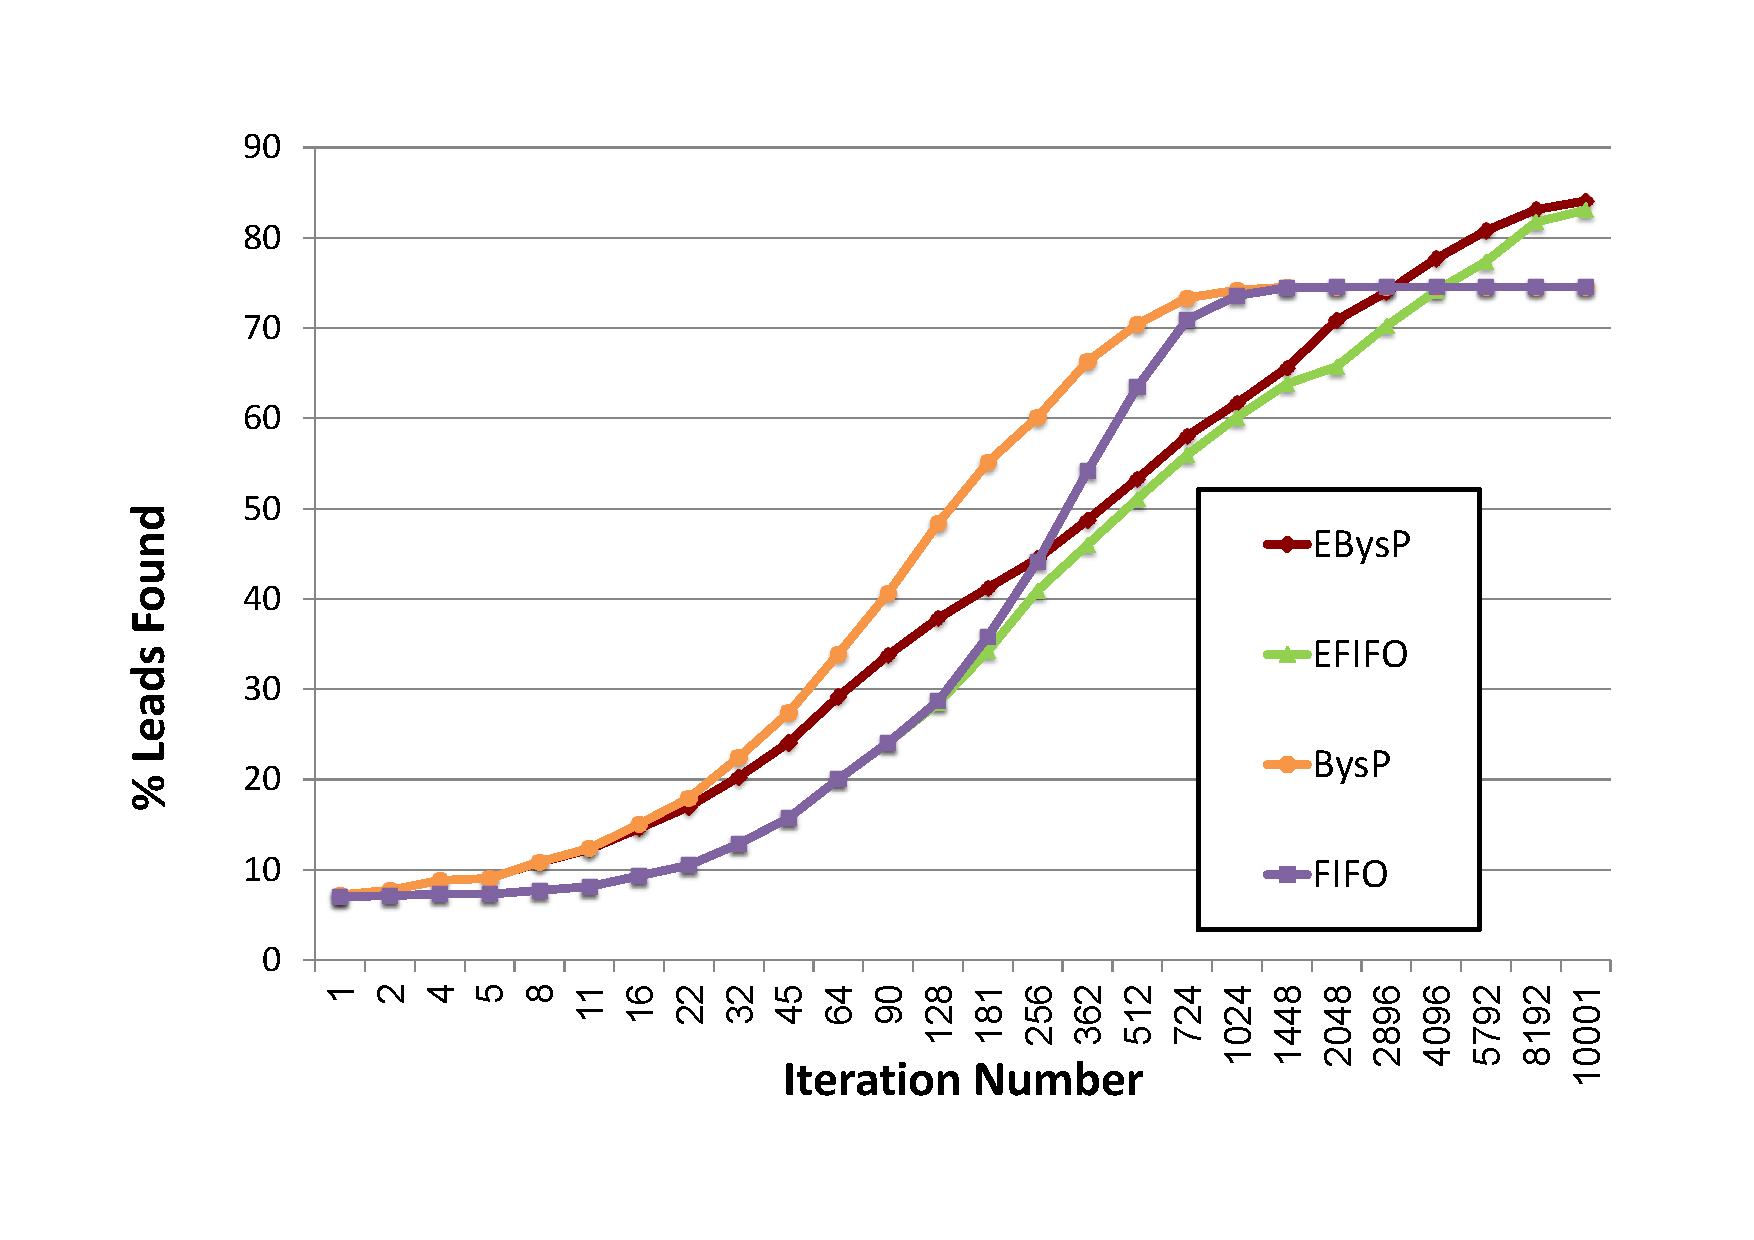
\includegraphics[width=\linewidth]{dblp_10k.pdf}%\vspace{-0.3cm}
% \caption{\label{fig:dblp}\% of leads found vs. iteration in DBLP network
% number}%\vspace{-0.3cm}
% \end{figure}


% The results are presented in Figure~\ref{fig:dblp}. An interesting observation that can be made from the figure is that the search is divided into three stages. (1) The beginning of the search in which the ETF heuristics preform similar to the RTF heuristic. (2) The second stage is the stage starting from the point in which the ETF and RTF heuristics cease to preform similarly and the RTF heuristics outperform the ETF heuristics. (3) The last stage is the stage in which the RTF heuristics have already found all of their reachable leads and the ETF heuristic continue to find new leads.

% At the first stage, the CKG is relatively small and the information obtained on the OSN topology is still insufficient to cause different choices of $best$ profiles between the RTF and ETF heuristics.


% In the third stage, we can see that the ETF heuristics continue to find leads after the RTF heuristics already found all of their reachable leads. Meaning that the use of ETF heuristics finds more leads than RTF, as can be expected from the Google+ results.


% The second stage is the most interesting stage. In this stage, EBysP does not outperform BysP as expected from the Google+ results previously shown.
% % Instead it appears as if the EBysP has chosen profiles that caused the search to scatter.

% To understand the differences between the networks, we have experimented with various topology attributes including the {\em clustering coefficient} (CC) of each target, the size of the {\em relem''vant neighborhood} of the target, the number of connected components in the graph excluding the target and the density of this neighborhood. The topology characteristic that has the most distinct impact on the proposed heuristics was the number of connected components in the graph (excluding the target).

% %The decrease resulted in new leads.
% We have checked the number of connected components in ETF(0) (RTF) and in ETF(1). As expected we have seen a decrease in the number of connected components between ETF(0) and ETF(1) both in Google+ and in DBLP. This decrease is caused since the additional tier in EFT(1) contains profiles that connect several connected components in ETF(0). Meaning, ETF(1) contains non leads that connect several connected components. 
% We noticed that the decrese was different between the Google+ and the DBLP networks. In Google+ the decreses was larger than in DBLP (40\% decrease from 15.94 to 9.3 connected components in Google+ as oppose to 30\% decrease from 6.29 to 4.38 connected components in DBLP).

% The non leads in ETF(1) can connect not only existing connected components, that were reachable in ETF(0) (from different initial leads), but also new connected components that were not reachable in ETF(0) and might contain leads. In fact, since ETF find more leads than RTF, as can be seen in the third stage, we know that new connected components containing leads were added to the graph in ETF(1) and are now reachable.

% %ETF has an advantage because it can search for both the old and the new leads
% Due to this decrease, ETF in general and EbysP in particular have the advantage of searching for leads in a larger variety of connected components. Meaning, that instead of focusing the search in the connected component that existed in ETF(0), the ETF heuristics can search for leads in the additional connected component if a lead is more likely to be found there. This advantage was the reason that EbysP preformed better than BysP even in the early stages of the search in the Google+ network. 

% %why does this adventage does not work in DBLP
% However, in DBLP, it is seems that EbysP does not have this advantage. In order to understand why, we have checked the number of reachable leads that were added into the graph in ETF(1). In Google+, 16.53\% new leads in average were added as oppose to 11.52\% new leads in DBLP. We have also checked the likelihood to find the new added lead by calculating the number of added reachable leads divided by all reachable profiles. The likelihood to find an added lead in Google+ is 0.01 as oppose to 0.007 in DBLP.
% Meaning that less leads were added in DBLP and that the likelihood of finding them is smaller than in Google+.
% This relatively small improvement in the number of reachable leads in DBLP, resulting from the relatively small decrease in the number of connected components, reduces the advantage that the ETF heuristics and EbysP in particular have, since the number of connected components to consider in ETF(1) is relatively similar to the number of connected components in ETF(0).
% In addition, the difference in the percentage of reachable leads between ETF(0) and ETF(1) is much lower in DBLP than in Google+. In Google+ the difference in the percentage of leads found is ~17.5\%(from 70\% to 88\% reachable leads) as oppose to only ~9\% (from 75\% to 84\% reachable leads).
% From this we conclude that in networks in which RTF finds a relatively large percentage of leads and the improvement in the percentage of reachable leads between ETF(0)  and ETF(1) is relatively low, such as DBLP, RTF heuristics will preform better during the run. By contrast, in networks such as Google+, in which RTF finds relatively lower percentage of leads and the improvement in the percentage of reachable leads between ETF(0) and ETF(1) is relatively high, ETF heuristics will preform better during the run.
% However, in both cases it is better to use ETF heuristics if we wish to find a larger number of leads.

% \note{Liron}{Write hybrid?}
% %%For that reasson we suggest, to use the hybrid heuristic presented in the paper in networks of the first kind (in which RTF preforms better). By using the hybrid heuristic, we can get the best prefermance by using BysP in the begining of the run in addition to finding more leads due to use of an ETF heuristic at the end of the run, as presented in Figure~.
% %Figure desc: 


\section{Experiments on Different Online Social Networks}
\label{sec:otherNetworks}
To provide further support for our conclusions, we also performed a series of experiments on other OSNs. Namely, we experimented on LiveJournal~\cite{backstrom2006groupFormation,leskovec2009community}, which is an online community that allows member to maintain journals, blogs, and define friendship between profiles, and Pokec~\cite{takac2012data}, which is the most popular OSN is Sloveniya. Both networks were made available as part of the Standform Network Analysis Project (SNAP) at \url{snap.stanford.edu}. Both OSNs are active and large (although not as large as Google+), where LiveJournal has more than 10 millions profiles and Pokec has more than 1.5 millions. 




. %We chose to compare only these algorithms as they represent two baseline approaches and the best performing heuristic found for Google+. 

\begin{figure}
\centering
\begin{subfigure}{.5\textwidth}
  \centering
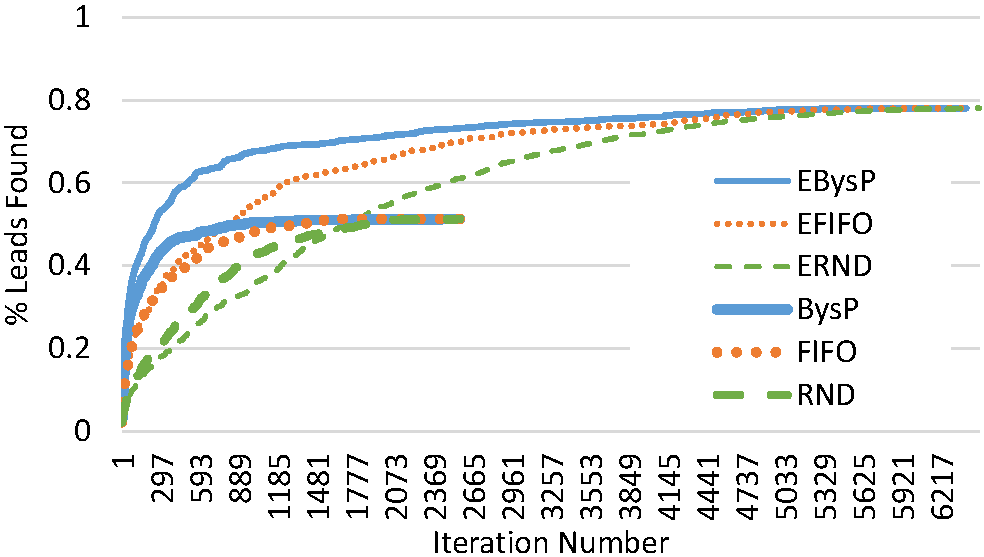
\includegraphics[width=\linewidth]{LiveJournal_cropped}
\caption{The Live Journal OSN}
\label{fig:live-journal}
\end{subfigure}%
\begin{subfigure}{.5\textwidth}
  \centering
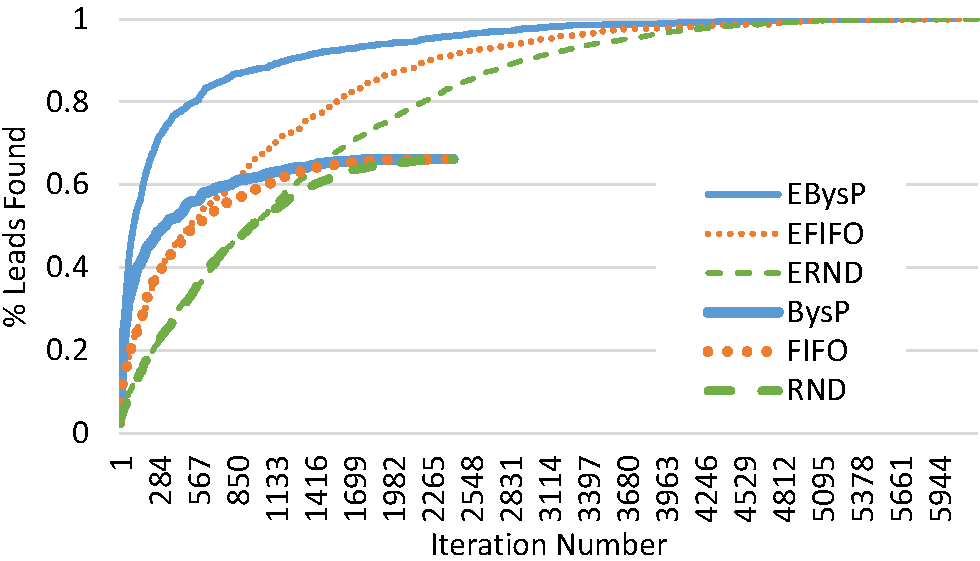
\includegraphics[width=\linewidth]{Pokec_cropped}
\caption{The Pokec OSN}
\label{fig:pokec}
\end{subfigure}
\caption{Evaluating TONIC heuristics on different OSNs.}
\label{fig:extra-osns}
\end{figure}

For each network we chosen randomly 50 profiles as targets, considering only profiles with more than 30 friends and 4,000 edges in its 2-tier neighborhood. For each target we present results for both TONIC frameworks (RTF and ETF)
and compare the baseline approaches random and FIFO with the best performing heuristic BysP. 

Figure~\ref{fig:extra-osns} shows the results for these two OSNs, in the same format as in Figure~\ref{fig:efm-and-ebysp}: the $x$-axis is the number of iterations and the $y$-axis is the percentage of leads found. The main trends observed for Google+ are seen here too:
\begin{itemize}
\item {\bf RTF finds fewer profiles.} The RTF algorithms exhausts the set of leads they can find and converges to finding fewer leads than the ETF algorithm.
\item {\bf BysP and EBysP dominate the baseline methods.} For both OSNs, BysP is better than random and FIFO, and EBysP is better than ETF random and EFIFO. 
\item {\bf EBysP dominates BysP.} Even before RTF exhausts all the leads it can reach, we observe that EBysP is able to find more leads faster than BysP. To demonstrate this, the average percentage of leads found after after 200 iterations was 45\% and 64\% for BysP and EBysP, respectively, in the Pokec OSN, and 39\% and 47\% for BysP and EBysP, respectively, in the Live Journal OSN. 
\end{itemize}




\begin{table}
\centering
\begin{tabular}{c|c|c|c}
Framework & Google+ & Pokec & Live Journal \\ \hline
RTF & 0.82 & 0.66 & 0.51 \\ 
ETF & 1.00 & 1.00 & 0.78 \\
\end{tabular}
\caption{\% of leads reachable with RTF and ETF in different OSNs.}
\label{tab:tiers-other-osns}
\end{table}

It is also interesting to compare the behavior of the different frameworks -- RTF and ETF -- across the three OSNs we experimented with (Google+, Pokec, and Live Journal). Table~\ref{tab:tiers-other-osns} shows the average percentage of reachable leads found using RTF and ETF for our OSNs. We observe that Live Journal OSN is the most difficult in terms of TONIC, in the sense that RTF and even ETF ends up finding fewer percentage of leads compared Google+ and Pokec. Indeed, the observant reader will see that the ETF algorithms in Figure~\ref{fig:live-journal} do not converge to finding all leads. This suggests future research in which the limitation of ETF to the first tier will be reevaluated based on the OSN characteristics. 

%This corresponds to comparing the size of tier zero and one in Table~\ref{tab:tiers}. We can see that Live Journal is the the most difficult OSN, in the sense that 
%The observant reader will notice that  for Live Journal, the ETF algorithms do not converge to finding all leads. This is because in Live Journal, running ETF(1) is not sufficient to find all leads from the initial leads, and exploring further tiers may be useful. Indeed, we also observe that the RTF algorithms for Live Journal also converge to finding a lower percentage of the target's lead, suggesting that the Live Journal OSN is sparser. To support this, Table~\ref{tab:tiers-other-osns} shows the average percentage of leads reachable using RTF and BTF for Google+, Pokec, and Live Journal. We can observe that Google+ has higher reachability 





%The proposed heuristics and frameworks are experimentally evaluated on three OSNs: Google+, Pokec~\cite{takac2012data}, and LiveJournal~\cite{backstrom2006groupFormation,leskovec2009community} (an online commmunity that allows member to maintain journals, blogs, and define friendship between profiles). Results show that each framework performs best in different circumstances. We found that in general \(RTF\) and \(ETF(1)\) are worthwhile while  ETF($n$) for $n>1$ does not contribute significantly to the number of leads found. We further analyze the trade-off between the cost of searching and the benefit of finding more leads. The results of this analysis show that \(ETF(1)\), with the proposed heuristics, is better than \(RTF\) for short searches and when the reward for finding a lead is high; while \(RTF\), with a proper heuristic, is better suited for a long term search process with moderate and low rewards. 
%\note{Roni}{TODO: Double check this after reading the results}


%Pokec is the most popular on-line social network in Slovakia. The popularity of network has not changed even after the coming of Facebook. Pokec has been provided for more than 10 years and connects more than 1.6 million people. Datasets contains anonymized data of the whole network. Profile data contains gender, age, hobbies, interest, education etc. Profile data are in Slovak language. Friendships in Pokec are oriented

%LiveJournal is a free on-line community with almost 10 million members; a significant fraction of these members are highly active. (For example, roughly 300,000 update their content in any given 24-hour period.) LiveJournal allows members to maintain journals, individual and group blogs, and it allows people to declare which other members are their friends they belong.

\section{Conclusion and Future Work}
%\subsection{RTF Conclusion and future work}
\label{sec:conclusions}

%\note{Roni}{Due to incomplete results, conclusions are not done yet}

This paper addressed the Target Oriented Network Intelligence Collection (TONIC) problem, in which the task is to find profiles in an OSN that contain information about a given target profile. Beyond academic interest, TONIC is an integral part of commercial and governmental applications.
TONIC was formalized as a search problem in an unknown graph and two frameworks for solving it were proposed, RTF and ETF. RTF focuses the search by only acquiring leads. ETF generalizes RTF by allowing non leads to be acquired, as long as there exists a known path from them to a lead that is at most $n$ hops long, where $n$ is a parameter. As $n$ grows, more leads are reachable but the search may become too costly and unfocused. Empirical results suggests that $n=1$ serves as a valid middle ground.

For both RTF and ETF(1), we present several heuristics for guiding the search. These heuristics are evaluated experimentally on a real OSN. 
Evaluation results show that:

\begin{enumerate}
\item The Bayesian Promising (BysP and EBysP) heuristics and the heuristics based on the Friends Measure, significantly outperform other heuristics.
\item Using ETF results in substantially more leads than RTF when using the anytime objective. 
\item Depending on the costs of the queries and on the reward of finding leads, either BysP (RTF) or EBysP (ETF(1)) is the preferable when using the MaxGain objective.
\item The number of reachable leads increases with both the number of initial leads and tier. 
\end{enumerate}

%We have also examined two social networks: Google+ and dblp.
%\note{Liron}{after the dblp is done, i need to talk about it here}\note{Roni}{Yes, need to be discussed.}

%Based on the evidence provided in this paper for both RTF and ETF(1) we suggest obtaining 2-3 initial leads with different kinds of acquaintances with the target. For example, one family member, one co-worker, and one blog fan.  \note{Roni}{This is just a statement without any backing up in our experiments. We have not checked where the initial leads come from or how different they are.}


There are many exciting directions for future work.
An obvious future work is to evaluate the proposed algorithms on different OSNs, and studying how properties of a given OSN affect their performance. 
Another future research direction is to create heuristics that consider a profile's textual data (hobbies, demographic information, etc.) and not just the topology of the CKG as the current heuristics do.
One other direction is to utilize the power of machine learning to predict which potential leads will turn to be leads de facto.
ML models can be trained using both data from past executions on various targets and data on profiles acquired during investigation of current target. 
% [R 2.2]
For example, one can learn a more sophisticated hybrid approach that combines information from several TONIC heuristics. 

% Costs, rewards, and uncertainty
Another direction is to consider leads with different rewards, where finding a lead that provides more information about \target\ is preferred. 
% [R 3.2]
In addition, one may consider higher cost for querying some profiles, e.g., to avoid querying profiles that are more sensitive and thus querying them is more risky. This raises a complex task of how to quantify information and how to quantify risk. Furthermore, information found from one lead can affect the value of information from other leads, as some information may overlap. In addition, we assumed that \islead{} and \acquire{} are always applicable. Future work can consider network errors that may cause queries to fail with some probability, introducing uncertainty.




\section{Ethical Aspects in TONIC}
\label{sec:ethics}
%[R 1.24]

As mentioned earlier in this paper, a particular application of our investigation of efficient TONIC solvers it to uncover the LOF of a target profile 
by exploring the LOFs of other profiles. Consequently, an efficient TONIC solver may uncover a target's LOF even if the target has blocked direct access to its LOF through its profile. Although this information (other profiles LOF) is publicly available, the ability to automatically and efficiently access this information raises some ethical concerns. 
First, one may argue that if the target has blocked access to its LOF, then by searching for its LOF we are accessing to the target's private information, even if the search itself is not done on the target but on other profiles. 
Second, one can imagine settings in which criminals use the proposed algorithm to collect information about citizens for various criminal activities. 

Indeed both concerns are valid and need to be discussed. It is general knowledge that people and organization use OSNs and other publicly available sources to gather information about specific entities (e.g., people, organizations, and other social groups). This is often done manually, for example, before hiring a person, 
or when police forces monitoring affiliates of known criminals in social networks. 
In fact, there are existing tools such as Palantir (\url{www.palantir.com}) that automatically collects publicly available information on a given profile. In that sense, our work is a more efficient version of an existing approach (which usually applies a FIFO strategy, which we show to be inferior). 


Moreover, we emphasize that an efficient TONIC solver can be used for many good purposes. It can serve as an helpful tool for law enforcement agencies. For example, imagine a search for information about a pedophile in an OSN. In fact, the social network paradigm has been successfully used to investigate organized crime in the Netherlands \cite{klerks2001network}. Alternatively, an efficient TONIC solver can be used as a tool for preserving privacy, by allowing a person to find how much publicly available information exists about him/her in a given OSN and change his/her privacy setting accordingly. 
Indeed, like many other advances in science the algorithms we propose can be used for good and bad purposes, depending on its user. 



\bibliographystyle{ACM-Reference-Format-Journals}

\bibliography{main}
 




\end{document}